\documentclass[letterpaper, 10pt, openright]{memoir}
\usepackage{fontspec}
\setmainfont{Liberation Serif}
\setlrmarginsandblock{3.5cm}{2.5cm}{*}
\setulmarginsandblock{2.3cm}{*}{1}
\checkandfixthelayout

%0ther
\renewcommand{\and}{\\\vskip 1em}
\def\headline#1{\hbox to \hsize{\hrulefill\quad\lower.3em\hbox{#1}\quad\hrulefill}}
\newcommand{\doendnotes}{%
	\markright{Notes}
	\theendnotes
	\setcounter{endnote}{0}
}
\newcommand{\doubleline}{%
	\hrule height 3\normalrulethickness
	\vskip 0.25em
	\hrule height \normalrulethickness
}

%Table of Contents
\makeatletter
\def\cftsectionpresnum #1\@cftasnum{}
\makeatother
\setlength\cftchapternumwidth{3em}
\cftpagenumbersoff{chapter}
\renewcommand{\contentsname}{\huge{Table} \Large{of} \huge{Contents}}

%Chapter style
\makechapterstyle{custom} {%
	\renewcommand{\thechapter}{\Roman{chapter}}
	\renewcommand{\chapterheadstart}{}
	\renewcommand{\printchaptername}{}
	\renewcommand{\chapternamenum}{}
	\renewcommand{\printchapternum}{\headline{\huge Chapter \thechapter}}
	\renewcommand{\afterchapternum}{%
		\vspace{1mm}}
	\renewcommand{\printchaptertitle}[1]{%
		\raggedright\huge\scshape{##1}}
	\renewcommand{\afterchaptertitle}{%
		\vskip\onelineskip \hrule\vskip\onelineskip}
}
\chapterstyle{custom}
\setcounter{chapter}{15}

%Section
\renewcommand{\thesection}{\Roman{section}}
\setsecheadstyle{\raggedright\scshape\large}
\setbeforesecskip{-\onelineskip}
\setaftersecskip{\onelineskip}
\setsecnumformat{}
\renewcommand{\sectionmark}[1]{\markboth{Chapter \thechapter.}{Part \thesection.}}

%subsection
\setsubsecheadstyle{\sethangfrom{\noindent ##1}\raggedright\itshape}
\setbeforesubsecskip{-\onelineskip}
\setaftersubsecskip{\onelineskip}

%EndNotes
\makepagenote
\renewcommand{\idtextinnotes}[1]{\footnotesize#1)\space}
\renewcommand{\prenoteinnotes}{\par\noindent\hangindent 2em}
\renewcommand{\prenotetext}{\begingroup\footnotesize}
\renewcommand{\postnotetext}{\endgroup}
\renewcommand{\notedivision}{%
	\headline{\huge\notesname}\vskip\onelineskip
	\markboth{Chapter \thechapter.}{\notesname}
	\thispagestyle{simple}
}
\renewcommand{\pagenotesubhead}[3]{}

\begin{document}
\frontmatter
\pretitle{\begin{center}\bfseries}
\title{%
	\small{THE}\\\vskip 1em
	\Huge{HISTORY}\\\vskip 1em
	\small{OF THE}\\\vskip 1em
	\Large{DECLINE AND FALL}\\\vskip 1em
	\small{OF THE}\\\vskip 1em
	\Huge{ROMAN EMPIRE}
}
\posttitle{\end{center}\vskip 1em}
\preauthor{\begin{center}\large\bfseries}
\author{%
	Edward Gibbon, \textit{Esq.}
	\and  With notes by the Rev. H. H. Milman
	\and Vol. 1}
\postauthor{\end{center}}
\predate{\begin{center}}
\date{\bfseries\normalsize 1782 (Written), 1845 (Revised)}
\postdate{%
	\end{center}
	\vskip 1em
	\doubleline
}

\maketitle


\tableofcontents*

\mainmatter
\chapter{ADAM'S PLACE IN THE EARTH'S DESTINY—2}

IN the Doctrine and Covenants, Section 107, we have a wonderful revelation on Priesthood.
This revelation was given at the request of the recently ordained apostles. They were about to
go forth on missions assigned to them and they desired some guidance by revelation, so the
Lord granted this request and instructed them in matters pertaining to the Priesthood. In the
course of this divine communication the Lord gave definite instruction in relation to Adam
and the patriarchs living before the flood. In it we are informed that the Priesthood was first
given to Adam and he in the course of years, ordained his son Seth, Enos, Cainan,
Mahalaleel, Jared, Enoch and Methuselah. Be it remembered that Adam, after the fall, lived
for 930 years. Seth ordained Lamech and Noah was ordained by Methuselah. This is the
descent of Priesthood from the beginning to the time of the flood.

Three years before the death of Adam, or in the year 927 from the date of the fall, this great
Patriarch and father of the human family called Seth, Enos, Cainan, Mahaleel, Jared, Enoch
and Methuselah, who were all high priests, with the residue of his faithful descendants, now
numerous, into the valley of Adam-ondi-Ahman, the place where Adam dwelt, and there
bestowed upon them his last blessing.

And the Lord appeared unto them, and they rose up and blessed Adam, and called him
Michael, the prince, the archangel.

And the Lord administered comfort unto Adam, and said unto him: I have set thee to be at
the head; a multitude of nations shall come of thee, and thou art a prince over them forever.

And Adam stood up in the midst of the congregation; and, notwithstanding he was bowed
down with age, being full of the Holy Ghost, predicted whatsoever should befall his posterity
unto the latest generation.

These things were all written in the book of Enoch, and are to be testified of in due time. 1

Again in Section 84, we have another reference to the descent of the Priesthood, this time
tracing it back from Moses, Abraham, Melchizedek, Noah, Enoch, Able to Adam, and in
verses 16 and 17 we read:

And from Enoch to Abel, who was slain by the conspiracy of his brother, who received the
priesthood by the commandments of God, by the hand of his father Adam, \textit{who was the first
man—}

Which priesthood continueth in the church of God in all generations, and is without
beginning of days or end of years.

We are here informed again that Adam was the first man, and that the Priesthood held by the
prophets of old came down through his lineage from him to the days of Moses, and from
Moses it continued on to the days of the coming of our Lord and Savior Jesus Christ. In the
Doctrine and Covenants, Section 117, we are informed that Adam dwelt in Adam-ondi-Ahman and the plains of Olaha Shinehah, which places have been made known to have been
on the western hemisphere, and in what is now known as the State of Missouri. This is well
for us to remember since it is the general impression that civilization commenced on the
eastern hemisphere. Then, in a revelation given to President Brigham Young at Winter
Quarters, January 14, 1847, the Lord said:

For they killed the prophets, and them that were sent unto them; and they have shed innocent
blood, which crieth from the ground against them.

Therefore, marvel not at these things, for ye are not yet pure; ye cannot yet bear my glory;
but ye shall behold it if ye are faithful in keeping all my words that I have given you, from
the days of Adam to Abraham, from Abraham to Moses, from Moses to Jesus and his
apostles, and from Jesus and his apostles to Joseph Smith, whom I did call upon by mine
angels, my ministering servants, and by mine own voice out of the heavens, to bring forth my
work. 2

I have now given testimony from the Pearl of Great Price, the Book of Mormon and the
Doctrine and Covenants, all confirming what is written in the Bible in regard to Adam, his
creation, his fall, his Priesthood, and indicating to us a very definite time when he lived; of
his ministry and when he died in full fellowship with the Lord, honored by his righteous
posterity. One other passage completes this list, that from Section 78, verses 15-16:

That you may come up unto the crown prepared for you, and be made rulers over many
kingdoms, saith the Lord God, the Holy One of Zion, who hath established the foundations of
Adam-ondi-Ahman; Who hath appointed Michael your prince, and established his feet, and
set him upon high, and given unto him the keys of salvation under the counsel and direction
of the Holy One, who is without beginning of days or end of life.

In this scripture we receive the knowledge that Michael, who is Adam, not only stands at the
head ruling over his posterity as a prince unto them forever; but also he has been appointed to
hold the keys of salvation for the benefit of the people of all the world who will truly repent
and receive the Gospel, and this great honor is bestowed upon him to act under the direction
of Jesus Christ who is the Only Begotten Son of God and the Holy One of Israel. Therefore,
all ye mockers and you mighty men take heed unto yourselves, for the day will come when
you will have to face this first man who has been crowned with honor to stand next to Jesus
Christ holding the keys of salvation; and you will not pass through the gates into that
kingdom without his consent! When that day comes and if you are permitted to pass through
those gates it will be only because you sorely repented and have humbly apologized to this
great man whom you have so mercilessly maligned.

The following teachings in regard to Adam are taken from the discourses and writings of the
Prophet Joseph Smith, who was better prepared to speak than any other man since the days of
Jesus Christ, on the life and authority of Adam. His knowledge was not obtained from books
or the writings of the worldly wise of the present day. What he learned and revealed was
given him by divine revelation.

The Prophet Joseph Smith had this to say about Adam and the Priesthood:

The Priesthood was first given to Adam; he obtained the First Presidency, and held the keys
of it from generation to generation. He obtained it in the Creation, before the world was
formed, as in Genesis 1:26, 27, 28. He had dominion given him over every living creature.
He is Michael the Archangel, spoken of in the scriptures. Then to Noah, who is Gabriel; he
stands next in authority to Adam in the Priesthood; he was called of God to this office, and
was the father of all living in his day, and to him was given the dominion. These men held
keys first on earth, and then in heaven.

The Priesthood is an everlasting principle, and existed with God from eternity, and will to
eternity, without beginning of days or end of years. The keys have to be brought from heaven
whenever the Gospel is sent. When they are revealed from heaven, it is by Adam's authority.

Daniel in his seventh chapter speaks of the Ancient of Days; he means the oldest man, our
Father Adam, Michael, he will call his children together and hold a council with them to
prepare them for the coming of the Son of Man. He (Adam) is the father of the human
family, and presides over the spirits of all men, and all that have had the keys must stand
before him in this grand council. This may take place before some of us leave this stage of
action. The Son of Man stands before him, and here is given him glory and dominion. Adam
delivers up his stewardship to Christ, that which was delivered to him as holding the keys of
the universe, but retains his standing as head of the human family.

The spirit of man is not a created being; it existed from eternity, and will exist to eternity.
Anything created cannot be eternal; and earth, water, etc., had their existence in an
elementary state, from eternity. Our Savior speaks of children and says, Their angels always
stand before my Father. The Father called all spirits before him at the creation of man, and
organized them. He (Adam) is the head and was told to multiply. The keys were first given to
him, and by him to others. He will have to give an account of his stewardship, and they to
him.

The Priesthood is everlasting. The Savior, Moses, and Elias, gave the keys to Peter, James
and John, on the mount, when they were transfigured before him. The Priesthood is
everlasting—without beginning of days or end of years; without father, mother, etc. If there
is no change of ordinances, there is no change of Priesthood. Wherever the ordinances of the
Gospel are administered, there is the Priesthood.

DESCENT OF PRIESTHOOD

How have we come at the Priesthood in the last days? It came down, in regular succession.
Peter, James and John, had it given to them and they gave it to others. Christ is the Great
High Priest; Adam next. Paul speaks of the Church coming to an innumerable company of
angels . . . to God the Judge of all—the spirits of just men made perfect; to Jesus the mediator
of the new covenant. (Hebrews 12:23.)

I saw Adam in the valley of Adam-ondi-Ahman. He called together his children and blessed
them with a patriarchal blessing. The Lord appeared in their midst, and he (Adam) blessed
them all, and foretold what would befall them to the latest generation.

This is why Adam blessed his posterity; he wanted to bring them into the presence of God.
They looked for a city, etc., "whose builder and maker is God." (Hebrews 11:10.) Mosessought to bring the children of Israel into the presence of God, through the power of the
Priesthood, but he could not. \textit{In the first ages of the world} they tried to establish the same
thing; and there were Eliases raised up who tried to restore these very glories, but did not
obtain them; but they prophesied of a day when this glory would be revealed. Paul spoke of
the dispensation of the fulness of times, when God would gather together all things in one,
etc.; and those men to whom these keys have been given, will have to be there; and they
without us cannot be made perfect.

These men are in heaven, but their children are on the earth. Their bowels yearn over us. God
sends down men for this reason. "The Son of man shall send forth his angels, and they shall
gather out of his kingdom all things that offend, and them which do iniquity." (Matthew
13:41.) All these authoritative characters will come down and join hand in hand in bringing
about this work. 3

At the October conference in Nauvoo in 1840, the Prophet gave further instruction regarding
the Priesthood and in the course of his remarks had the following to say about Adam:

Commencing with Adam, who was the first man, who is spoken of in Daniel as being the
"Ancient of Days," or in other words, the first and oldest of all, the great, grand progenitor of
whom it is said in another place he is Michael, because he was the first and father of all, not
only by progeny, but the first to hold the spiritual blessings, to whom was made known the
plan of ordinances for the salvation of his posterity unto the end, and to whom Christ was
first revealed, and through whom Christ has been revealed from heaven, and will continue to
be revealed from henceforth. Adam holds the keys of the dispensation of the fulness of times;
i.e., the dispensation of all the times have been and will be revealed through him from the
beginning to Christ, and from Christ to the end of the dispensations that are to be revealed.
"Having made known unto us the mystery of his will, according to his good pleasure which
he hath purposed in himself: That in the dispensation of the fulness of times he might gather
together in one all things in Christ, both which are in heaven, and which are on earth; even in
him." (Eph. 1:9-10.)

Now the purpose in himself in the winding up scene of the last dispensation is that all things
pertaining to that dispensation should be conducted precisely in accordance with the
preceding dispensations.

And again, God purposed in himself that there should not be an eternal fulness until every
dispensation should be fulfilled and gathered together in one, and that all things whatever,
that should be gathered together in one in those dispensations unto the same fulness and
eternal glory, should be in Christ Jesus; therefore he set the ordinances to be the same forever
and ever, and set Adam to watch over them, to reveal them from heaven to man, or to send
angels to reveal them. "Are they not all ministering spirits, sent forth to minister for them
who shall be heirs of salvation?" (Hebrews 1:14.)

These angels are under the direction of Michael or Adam, who acts under the direction of the
Lord. From the above quotation we learn that Paul perfectly understood the purposes of God
in relation to his connection with man, and that glorious and perfect order which he
established in himself, whereby he sent forth power, revelations, and glory.

ADAM RECEIVED COMMANDMENTS FROM GOD

God will not acknowledge that which he has not called, ordained, and chosen. In the
beginning God called Adam by his own voice. "And the Lord God called unto Adam, and
said unto him, Where art thou? And he said, I heard thy voice in the garden, and I was afraid
because I was naked; and hid myself." (Genesis 3:9-10.) Adam received commandments and
instructions from God: this was the order from the beginning.

That he received revelations, commandments and ordinances at the beginning is beyond the
power of controversy; else how did they begin to offer sacrifices to God in an acceptable
manner. And if they offered sacrifices they must be authorized by ordination. We read in
Genesis 4:4, that Abel brought of the firstlings of the flock and the fat thereof, and the Lord
had respect to Abel and to his offering. And, again, "By faith Abel offered unto God a more
excellent sacrifice than Cain, by which he obtained witness that he was righteous, God
testifying of his gifts: and by it he being dead yet speaketh." (Hebrews 11:4.) How doth he
yet speak? Why he magnified the Priesthood which was conferred upon him, and died a
righteous man, and therefore has become an angel of God by receiving his body from the
dead, holding still the keys of his dispensation; and was sent down from heaven unto Paul to
minister consoling words, and to commit unto him a knowledge of the mysteries of
godliness.

And if this was not the case, I would ask, how did Paul know so much about Abel, and why
should he talk about his speaking after he was dead? Hence, that he spoke after he was dead
must be by being sent down out of heaven to administer.

This, then, is the nature of the Priesthood; every man holding the Presidency of his
dispensation, and one man holding the Presidency of them all, even Adam; and Adam
receiving his Presidency and authority from the Lord, but cannot receive a fulness until
Christ shall present the kingdom to the Father, which shall be at the end of the last
dispensation. . . .

If Cain had fulfilled the law of righteousness as did Enoch, he could have walked with God
all the days of his life, and never failed of a blessing. "And Enoch walked with God after he
begat Methuselah three hundred years, and begat sons and daughters: And all the days of
Enoch were three hundred sixty and five years: And Enoch walked with God, and he was not,
for God took him." (Gen. 5:22-24.) Now this Enoch God reserved unto himself, that he
should not die at that time, and appointed unto him a ministry unto terrestrial bodies, of
whom there has been little revealed. He is reserved also unto the presidency of a
dispensation, and more shall be said of him and terrestrial bodies in another treatise. He is a
ministering angel, to minister to those who shall be heirs of salvation, and appeared unto
Jude as Abel did unto Paul; therefore Jude spoke of him (14-15 verses). And Enoch, the
seventh from Adam, revealed these sayings: "Behold, the Lord cometh with ten thousands of
his saints." 4

In the early part of the year 1912, Elder Samuel O. Bennion, then presiding in the Central
States Mission, wrote to the First Presidency for a statement answering the enemies of the
Church who were falsely quoting President Brigham Young. The letter of Presidency to
Elder Bennion is as follows:

Salt Lake City, Utah

February 20, 1912

Pres. Samuel O. Bennion,

Independence, Missouri.

Dear Brother:

Your question concerning Adam has not been answered because of pressure of important
business. We now respond briefly but, we hope, plainly. You speak of "the assertion made by
Brigham Young that Jesus was begotten of the Father in the flesh by our father Adam, and
that Adam is the father of Jesus Christ and not the Holy Ghost, and you say that elders are
challenged by certain critics to prove this.

If you will carefully examine the sermon to which you refer, in the \textit{Journal of Discourses,}
Vol. 1, you will discover that, while President Young denied that Jesus was "begotten by the
Holy Ghost," he did not affirm, in so many words, that "Adam is the father of Jesus Christ in
the flesh." He said, "Jesus, our elder brother, was begotten in the flesh by the same character
that was in the garden of Eden and who is our Father in Heaven." Here is what President
Young said about him, "Our Father in Heaven begat all the spirits that ever were or ever will
be upon this earth and they were born spirits in the eternal world. Then the Lord by his power
and wisdom organized the mortal tabernacle of man." Was he in the garden of Eden?

Surely; he gave commandment to Adam and Eve; he was their Father in Heaven; they
worshiped him and taught their children after the fall to worship and obey him in the name of
the Son who was to come.

But President Young went on to show that our father Adam—that is, our earthly father—the
progenitor of the race of man, stands at the head, being "Michael the Archangel, the Ancient
of Days," and that he was not fashioned from earth like an adobe, but begotten by his Father
in Heaven.

Adam is called in the Bible "the son of God." (Luke 3:38.) It was our Father in Heaven who
begat the spirit of him who was the Firstborn of all spirits that come to this earth and who
was also his Father by the Virgin Mary, making him "the Only Begotten in the flesh." Read
Luke 1:26-35. Where is Jesus called "the Only Begotten of the Holy Ghost?" He is always
singled out as "the Only Begotten of the Father." (John 14:3-16-18, etc.). The Holy Ghost
came upon Mary, her conception was under that influence, even of the spirit of life; our
Father in Heaven was the Father of the Son of Mary, to whom the Savior prayed, as did our
earthly father Adam.

When President Young asked, "Who is the father?" he was speaking of Adam as the father of
our earthly bodies, who is at our head as revealed in Doctrine and Covenants, Sec. 107,
verses 53-56. In that sense he is one of the Gods referred to in numerous scriptures, and
particularly by Christ. (John 10:34-36.) He is the great Patriarch, the Ancient of Days, who
will stand in his place as "a prince over us forever," and with whom we shall have to do," as
each family will have to do with its head, according to the Holy Patriarchal order. Our father
Adam, perfected and glorified as a God, will be a being who will carry out the behests of the
great Elohim in relation to his posterity.

While, as Paul puts it, There be gods many and lords many (whether in heaven or in earth),
unto us there is but one God the Father, of whom are all things, and one Lord Jesus Christ.
Latter-day Saints worship him and him alone, who is the Father of Jesus Christ, whom he
worshiped, whom Adam worshiped and who is God the Eternal Father of us all.

Your brethren,

Joseph F. Smith

Anthon H. Lund

Charles W. Penrose

First Presidency President Brigham Young has borne testimony concerning Adam and his
place in the world as Michael, the Archangel, who will stand at the head of his posterity
forever having jurisdiction over them under Jesus Christ. In one of his discourses he said:

We are safe in saying that from the day that Adam was created and placed in the garden of
Eden to this day, the plan of salvation and the revelations of the will of God to man are
unchanged, although mankind have not for many ages been favored there-with, in
consequence of apostasy and wickedness. There is no evidence to be found in the Bible that
the Gospel should be one thing in the days of the Israelites, and another in the days of Christ
and his apostles, and another in the 19th century, but, on the contrary, we are instructed that
God is the same in every age, and that his plan of saving his children is the same. The plan of
salvation is one, from the beginning of the world to the end thereof. 5

Adam was as conversant with his Father who placed him upon the earth as we are conversant
with our earthly parents. The Father frequently came to visit his son Adam, and walked with
him; and the children of Adam were more or less acquainted with him; and the things that
pertain to God and to heaven were as familiar among mankind in the first ages of their
existence on the earth, as these mountains are to our mountain boys, as gardens are to our
wives and children, or as the road to the Western Ocean is to the experienced traveler. From
this source mankind received their religious traditions. 6

The youth of Israel should remember that the Prophet Joseph Smith was in communication
with the heavens constantly. He was instructed by angels and by the Son of God himself. For
four years he was tutored by the Angel Moroni before he was privileged to obtain the plates
of the Book of Mormon and after that he was frequently visited by heavenly messengers. He
and Oliver Cowdery stood in the presence of John the Baptist and under his hands received
the Aaronic Priesthood, and later under the hands of Peter, James and John received the
Melchizedek Priesthood and were commanded to organize the Church. The ancient prophets
from Adam to Peter, James and John in the dispensation of the Meridian of Time, came and
manifested the keys of their dispensations to these two men. The Prophet Joseph Smith saw
Adam as well as these many other ancient prophets; he speaks by authority for he had the
knowledge. He knew that Adam lived and that he is the "first man," the "Ancient of Days,"
so called because he was the "oldest of all." I have presented the testimonies of the Nephite
prophets, the ancient prophets of the Israelites as the knowledge has come to us through
revelation and recorded in the Pearl of Great Price and the writings of Abraham, all
confirming the stories related in the Bible. We discover that organic evolution mocks at all of
this.

Now, my beloved brethren and sisters, and especially you younger members of the Church, is
it not better to hearken to these brethren who had personal knowledge than to accept the
insecure doctrines of those who reject their Redeemer and his servants and endeavor to put
them to open shame?

\newpage
REFERENCES—CHAPTER SIXTEEN

Footnotes

1. D. \& C. 107:41-57.

2. \textit{Ibid.}, 136:36-37.

3. \textit{Teachings of the Prophet Joseph Smith}, pp. 157-159.

4. \textit{Ibid.}, pp. 167-170.

5. \textit{Journal of Discourses}, Vol. 10, p. 324.

6. \textit{Ibid.}, Vol. 9, p. 148.


\printpagenotes*
\chapter{ADAM'S PLACE IN THE EARTH'S DESTINY—3}

THERE are other testimonies coming from our brethren, who were trained under the
teachings of the Prophet Joseph Smith and who are able to speak by virtue of the inspiration
of the Spirit of the Lord by which they have been led. Their teachings should be heeded by
the members of the Church. The following article by the First Presidency was written for the
purpose of directing our Church members in the light of revealed truth and to fortify them
against the false doctrines and philosophies so prevalent in the world.

THE ORIGIN OF MAN By THE FIRST PRESIDENCY OF THE CHURCH

\textit{"God created man in his own image."}

Inquiries arise from time to time respecting the attitude of the Church of Jesus Christ of
Latter-day Saints upon questions which, though not vital from a doctrinal standpoint, are
closely connected with the fundamental principles of salvation. The latest inquiry of this kind
that has reached us is in relation to the origin of man. It is believed that a statement of the
position held by the Church upon this important subject will be timely and productive of
good.

In presenting the statement that follows we are not conscious of putting forth anything
essentially new; neither is it our desire so to do. Truth is what we wish to present, and truth—
eternal truth—is fundamentally old. A restatement of the original attitude of the Church
relative to this matter is all that will be attempted here. To tell the truth as God has revealed
it, and commend it to the acceptance of those who need to conform their opinions thereto, is
the sole purpose of this presentation.

"God created man in his own image, in the image of God created he him; male and female
created he them." In these plain and pointed words the inspired author of the book of Genesis
made known to the world the truth concerning the origin of the human family. Moses, the
prophet-historian, "learned," as we are told, "in all the wisdom of the Egyptians," when
making this important announcement, was not voicing a mere opinion, a theory derived from
his researches into the occult lore of that ancient people. He was speaking as the mouthpiece
of God, and his solemn declaration was for all time and for all people. No subsequent
revelator of the truth has contradicted the great leader and law-giver of Israel. All who have
since spoken by divine authority upon this theme have confirmed his simple and sublime
proclamation. Nor could it be otherwise. Truth has but one source, and all revelations from
heaven are harmonious with each other. The omnipotent Creator, the maker of heaven and
earth—had shown unto Moses everything pertaining to this planet, including the facts
relating to man's origin, and the authoritative pronouncement of that mighty prophet and seer
to the house of Israel, and through Israel to the whole world, is couched in the simplest
clause: "God created man in his own Image." (Genesis 1:27; Pearl of Great Price—Book of
Moses, 1:27-41.)

The creation was two-fold—first spiritual, secondly temporal. This truth, also, Moses plainly
taught—much more plainly than it has come down to us in the imperfect translations of the
Bible that are now in use. Therein the fact of a spiritual creation, antedating the temporal
creation, is strongly implied, but the proof of it is not so clear and conclusive as in other
records held by the Latter-day Saints to be of equal authority with the Jewish scriptures. The
partial obscurity of the latter upon the point in question is owing, no doubt, to the loss of
those "plain and precious" parts of sacred writ, which, as the Book of Mormon informs us,
have been taken away from the Bible during its passage down the centuries. (1 Nephi 13:24-
29.) Some of these missing parts the Prophet Joseph Smith undertook to restore when he
revised those scriptures by the spirit of revelation, the result being that more complete
account of the creation which is found in the book of Moses, previously cited. Note the
following passages:

"And now, behold I say unto you, that these are the generations of the heaven and of the
earth, when they were created, in the day that I, the Lord God, made the heaven and the
earth:

"And every plant of the field before it was in the earth, and every herb of the field before it
grew. For I, the Lord God, created all things, of which I have spoken, spiritually, before they
were naturally upon the face of the earth. For I, the Lord God, had not caused it to rain upon
the face of the earth. And I, the Lord God, had created all the children of men, and not yet a
man to till the ground: for in heaven created I them; and there was not yet flesh upon the
earth, neither in the water, neither in the air:

"But I, the Lord God, spake, and there went up a mist from the earth, and watered the whole
face of the ground.

"And I, the Lord God, formed man from the dust of the ground, and breathed into his nostrils
the breath of life; and man became a living soul, the first flesh upon the earth, the first man
also; nevertheless, all things were before created; but spiritually were they created and made
according to my word." (Pearl of Great Price—Book of Moses, 3:4-7. See also chapters 1
and 2, and compare with Genesis 1 and 2.)

These two points being established, namely, the creation of man in the image of God, and the
two-fold character of the creation, let us now inquire: What was the form of man, in the spirit
and in the body, as originally created? In a general way the answer is given in the words
chosen as the text of this treatise. "God created man in his own image." It is more explicitly
rendered in the Book of Mormon thus: "All men were created in the beginning after mine
own image." (Ether 3:15.) It is the Father who is speaking. If, therefore, we can ascertain the
form of the "Father of spirits," "The God of the spirits of all flesh," we shall be able to
discover the form of the original man.

Jesus Christ, the Son of God, is "the express image" of his Father's person. (Hebrews 1:3.) He
walked the earth as a human being, as a perfect man, and said, in answer to a question put to
him: "He that hath seen me hath seen the Father." (John 14:9.) This alone ought to solve the
problem to the satisfaction of every thoughtful, reverent mind. The conclusion is irresistible,
that if the Son of God be the express image (that is, likeness) of his Father's person, then his
Father is in the form of man; for that was the form of the Son of God, not only during his
mortal life, but before his mortal birth, and after his resurrection. It was in this form that the
Father and the Son, as two personages, appeared to Joseph Smith, when, as a boy of fourteen
years, he received his first vision. Then if God made man—the first man—in his own image
and likeness, he must have made him like unto Christ, and consequently like unto men of
Christ's time and of the present day. That man was made in the image of Christ, is positively
stated in the book of Moses: "And I, God, said unto mine Only Begotten, which was with me
from the beginning: Let us make man in our image, after our likeness; and it was so. . . . And
I, God, created man in mine own image, in the image of mine Only Begotten created I him;
male and female created I them." (2:26, 27.)

The Father of Jesus is our Father also, Jesus himself taught this truth, when he instructed his
disciples how to pray: "Our Father which art in heaven," etc. Jesus, however, is the Firstborn
among all the sons of God—the first begotten in the spirit, and the Only Begotten in the
flesh. He is our elder brother, and we, like him, are in the image of God. All men and women
are in the similitude of the universal Father and Mother, and are literally the sons and
daughters of Deity.

"God created man in his own image." This is just as true of the spirit as it is of the body,
which is only the clothing of the spirit, its complement; the two together constituting the
soul. The spirit of man is in the form of man, and the spirits of all creatures are in the likeness
of their bodies. This was plainly taught by the Prophet Joseph Smith. (Doctrine and
Covenants, 77:2.)

Here is further evidence of the fact. More than seven hundred years before Moses was shown
the things pertaining to this earth, another great prophet, known to us as the brother of Jared,
was similarly favored by the Lord. He was even permitted to behold the spirit-body of the
foreordained Savior, prior to his incarnation; and so like the body of a man was his spirit in
form and appearance, that the prophet thought he was gazing upon a being of flesh and
blood. He first saw the finger and then the entire body of the Lord—all in the spirit. The
Book of Mormon says of this wonderful manifestation:

"And it came to pass that when the brother of Jared had said these words, behold, the Lord
stretched forth his hand and touched the stones one by one with his finger. And the veil was
taken from off the eyes of the brother of Jared, and he saw the finger of the Lord; and it was
as the finger of a man, like unto flesh and blood; and the brother of Jared fell down before the
Lord, for he was struck with fear.

"And the Lord saw that the brother of Jared had fallen to the earth; and the Lord said unto
him: Arise, why hast thou fallen?

"And he saith unto the Lord: I saw the finger of the Lord, and I feared lest he should smite
me; for I knew not that the Lord had flesh and blood.

"And the Lord said unto him: Because of thy faith thou hast seen that I shall take upon me
flesh and blood; and never has man come before me with such exceeding faith as thou hast;
for were it not so, ye could not have seen my finger. Sawest thou more than this?

"And he answered: Nay; Lord, show thyself unto me.

"And the Lord said unto him: Believest thou the words which I shall speak?

"And he answered: Yea, Lord, I know that thou speakest the truth, for thou art a God of truth,
and canst not lie.

"And when he had said these words, behold, the Lord showed himself unto him, and said:
Because thou knowest these things ye are redeemed from the fall; therefore ye are brought
back into my presence; therefore I show myself unto you.

"Behold, I am he who was prepared from the foundation of the world to redeem my people.
Behold, I am Jesus Christ. I am the Father and the Son. In me shall all mankind have light,
and that eternally, even they who shall believe on my name; and they shall become my sons
and my daughters.

"And never have I showed myself unto man whom I have created, for never has man
believed in me as thou hast. Seest thou that ye are created after mine own image? Yea, even
all men were created in the beginning after mine own image.

"Behold, this body, which ye now behold, is the body of my spirit; and man have I created
after the body of my spirit; and even as I appear unto thee to be in the spirit will I appear unto
my people in the flesh." (Ether 3:6-16.)

What more is needed to convince us that man, both in spirit and in body, is the image and
likeness of God, and that God himself is in the form of man?

When the divine Being whose spirit-body the brother of Jared beheld, took upon him flesh
and blood, he appeared as a man, having "body, parts and passions," like other men, though
vastly superior to all others, because he was God, even the Son of God, the Word made flesh:
in him "dwelt the fulness of the Godhead bodily." And why should he not appear as a man?
That was the form of his spirit, and it must needs have an appropriate covering, a suitable
tabernacle. He came into the world as he had promised to come (3 Nephi 1:13) taking an
infant tabernacle, and developing it gradually to the fulness of his spirit stature. He came as
man had been coming for ages, and as man has continued to come ever since. Jesus,
however, as shown, was the Only Begotten of God in the flesh.9

"Adam, our great progenitor, "the first man," was, like Christ, a pre-existent spirit, and like
Christ he took upon him an appropriate body, the body of a man, and so became a "living
soul." The doctrine of the pre-existence,—revealed so plainly, particularly in latter days,
pours a wonderful flood of light upon the otherwise mysterious problem of man's origin. It
shows that man, as a spirit, was begotten and born of heavenly parents, and reared to
maturity in the eternal mansions of the Father, prior to coming upon the earth in a temporal
body to undergo an experience in mortality. It teaches that all men existed in the spirit before
any man existed in the flesh, and that all who have inhabited the earth since Adam have taken
bodies and become souls in like manner.

It is held by some that Adam was not the first man upon this earth, and that the original
human being was a development from lower orders of the animal creation. These, however,
are the theories of men. The word of the Lord declares that Adam was "the first man of all
men" (Moses 1:34), and we are therefore in duty bound to regard him as the primal parent of
the race. It was shown to the brother of Jared that all men were created in the beginning after
the image of God; and whether we take this to mean the spirit or the body, or both, it
commits us to the same conclusion: Man began life as a human being, in the likeness of our
heavenly Father.

True it is that the body of man enters upon its career as a tiny germ or embryo, which
becomes an infant, quickened at a certain stage by the spirit whose tabernacle it is, and the
child, after being born, develops into a man. There is nothing in this, however, to indicate
that the original man, the first of our race, began life as anything less than a man, or less than
the human germ or embryo that becomes a man.

Man, by searching, cannot find out God. Never, unaided, will he discover the truth about the
beginning of human life. The Lord must reveal himself, or remain unrevealed; and the same
is true of the facts relating to the origin of Adam's race—God alone can reveal them. Some of
these facts, however, are already known, and what has been made known it is our duty to
receive and retain.

The Church of Jesus Christ of Latter-day Saints, basing its belief on divine revelation,
ancient and modern, proclaims man to be the direct and lineal offspring of Deity. God
himself is an exalted man, perfected, enthroned, and supreme. By his almighty power he
organized the earth, and all that it contains, from spirit and element, which exist co-eternally
with himself. He formed every plant that grows, and every animal that breathes, each after its
own kind, spiritually and temporally—"that which is spiritual being in the likeness of that
which is temporal, and that which is temporal in the likeness of that which is spiritual." He
made the tadpole and the ape, the lion and the elephant; but he did not make them in his own
image, nor endow them with Godlike reason and intelligence. Nevertheless, the whole animal
creation will be perfected and perpetuated in the hereafter, each class in its "distinct order or
sphere," and will enjoy "eternal felicity." That fact has been made plain in this dispensation.
(Doctrine and Covenants 77:3.)

Man is the child of God, formed in the divine image and endowed with divine attributes, and
even as the infant son of an earthly father and mother is capable in due time of becoming a
man, so the undeveloped offspring of celestial parentage is capable, by experience through
ages and aeons, of evolving into a God.

Joseph F. Smith

John R. Winder

Anthon H. Lund,

First Presidency of the Church of Jesus Christ of Latter-day Saints. 1

The word of the Lord in the Pearl of Great Price, the Book of Abraham, and the Doctrine and
Covenants, should carry enough weight with members of the Church to satisfy them and give
them a firm foundation on which to stand. To all the members who have received the
testimony through the Holy Ghost, these teachings supporting the Old Testament, will
suffice. We do have in the Church, however, a great many members who do not have that
abiding testimony, unfortunately. These are readily disturbed by the philosophies and
theories taught in the colleges and other schools and it is difficult for them to see that the
philosophical doctrines can be false. Many of the theories are proclaimed with such positive
finality that those weak in the faith are confused or perhaps inclined to accept the deductions
of these teachers and think that the revelations must be wrong. This is a step towards
apostasy. As the Lord declared, we cannot serve two masters. We cannot accept the
hypotheses of science which are in conflict with that which is here set forth in clearness, at
the same time. They are diametrically opposite to each other. Therefore it seems the part of
wisdom to present more testimony than is obtainable in the direct word of the Lord.
Therefore I shall proceed to present some of the writings of others of the members of the
Church who were schooled under the Prophet Joseph Smith. Here is a saying by President
Brigham Young:

It is a true saying of the Savior's . . . He came for the express purpose of dividing the
righteous from the wicked. This formed as much a part of his holy ministry as any other part
of the will of the Father.

We see this principle verified from days of old. It was demonstrated in the very
commencement of the peopling of the earth. How soon an opposition was introduced in the
morning of creation, when righteousness was proclaimed, when truth was revealed, when the
light and knowledge of eternity shone with lustrous beauty upon Adam and his children. Cain
must rise up and slay his brother while they were walking with the Lord. . . .

It is very true, had not sin entered into the world, and opposition been introduced, \textit{death
would not have entered.} (My italics.) From that time to this, death, opposition, selfishness,
malice, anger, pride, darkness of every description that could be invented by the children of
men, as they have multiplied and spread abroad in the earth, have increased. 2

How did Adam and Eve sin? Did they come out in direct opposition to God and to his
government? No. But they transgressed a command of the Lord, and through that
transgression sin came into the world. . . . Then came the curse upon the fruit, upon the
vegetables, and upon our mother earth; and it came upon the creeping things, upon the grain
in the field, the fish in the sea, and upon all things pertaining to this earth, through Man's
transgression. 3

\newpage
REFERENCES—CHAPTER SEVENTEEN

Footnotes

1. \textit{Improvement Era}, Vol. 13, pp. 75-81.

2. \textit{Journal of Discourses}, Vol. 1, pp. 234-5

3. \textit{Ibid.}, Vol. 10, p. 312.


\printpagenotes*
\chapter{The Treasure}

When Dantès returned next morning to the chamber of his companion in
captivity, he found Faria seated and looking composed. In the ray of
light which entered by the narrow window of his cell, he held open in
his left hand, of which alone, it will be recollected, he retained the
use, a sheet of paper, which, from being constantly rolled into a small
compass, had the form of a cylinder, and was not easily kept open. He
did not speak, but showed the paper to Dantès.

“What is that?” he inquired.

“Look at it,” said the abbé with a smile.

“I have looked at it with all possible attention,” said Dantès, “and I
only see a half-burnt paper, on which are traces of Gothic characters
inscribed with a peculiar kind of ink.”

“This paper, my friend,” said Faria, “I may now avow to you, since I
have the proof of your fidelity—this paper is my treasure, of which,
from this day forth, one-half belongs to you.”

The sweat started forth on Dantès’ brow. Until this day and for how
long a time!—he had refrained from talking of the treasure, which had
brought upon the abbé the accusation of madness. With his instinctive
delicacy Edmond had preferred avoiding any touch on this painful chord,
and Faria had been equally silent. He had taken the silence of the old
man for a return to reason; and now these few words uttered by Faria,
after so painful a crisis, seemed to indicate a serious relapse into
mental alienation.

“Your treasure?” stammered Dantès. Faria smiled.

“Yes,” said he. “You have, indeed, a noble nature, Edmond, and I see by
your paleness and agitation what is passing in your heart at this
moment. No, be assured, I am not mad. This treasure exists, Dantès, and
if I have not been allowed to possess it, you will. Yes—you. No one
would listen or believe me, because everyone thought me mad; but you,
who must know that I am not, listen to me, and believe me so afterwards
if you will.”

“Alas,” murmured Edmond to himself, “this is a terrible relapse! There
was only this blow wanting.” Then he said aloud, “My dear friend, your
attack has, perhaps, fatigued you; had you not better repose awhile?
Tomorrow, if you will, I will hear your narrative; but today I wish to
nurse you carefully. Besides,” he said, “a treasure is not a thing we
need hurry about.”

“On the contrary, it is a matter of the utmost importance, Edmond!”
replied the old man. “Who knows if tomorrow, or the next day after, the
third attack may not come on? and then must not all be over? Yes,
indeed, I have often thought with a bitter joy that these riches, which
would make the wealth of a dozen families, will be forever lost to
those men who persecute me. This idea was one of vengeance to me, and I
tasted it slowly in the night of my dungeon and the despair of my
captivity. But now I have forgiven the world for the love of you; now
that I see you, young and with a promising future,—now that I think of
all that may result to you in the good fortune of such a disclosure, I
shudder at any delay, and tremble lest I should not assure to one as
worthy as yourself the possession of so vast an amount of hidden
wealth.”

Edmond turned away his head with a sigh.

“You persist in your incredulity, Edmond,” continued Faria. “My words
have not convinced you. I see you require proofs. Well, then, read this
paper, which I have never shown to anyone.”

“Tomorrow, my dear friend,” said Edmond, desirous of not yielding to
the old man’s madness. “I thought it was understood that we should not
talk of that until tomorrow.”

“Then we will not talk of it until tomorrow; but read this paper
today.”

“I will not irritate him,” thought Edmond, and taking the paper, of
which half was wanting,—having been burnt, no doubt, by some
accident,—he read:

\vskip \onelineskip

\begin{quote}
{\small“this treasure, which may amount to two...

of Roman crowns in the most distant a...

of the second opening wh...

declare to belong to him alo...

heir.

\hspace{6em}“25th April, 149’”}
\end{quote}

\vskip \onelineskip

“Well!” said Faria, when the young man had finished reading it.

“Why,” replied Dantès, “I see nothing but broken lines and unconnected
words, which are rendered illegible by fire.”

“Yes, to you, my friend, who read them for the first time; but not for
me, who have grown pale over them by many nights’ study, and have
reconstructed every phrase, completed every thought.”

“And do you believe you have discovered the hidden meaning?”

“I am sure I have, and you shall judge for yourself; but first listen
to the history of this paper.”

“Silence!” exclaimed Dantès. “Steps approach—I go—adieu!”

And Dantès, happy to escape the history and explanation which would be
sure to confirm his belief in his friend’s mental instability, glided
like a snake along the narrow passage; while Faria, restored by his
alarm to a certain amount of activity, pushed the stone into place with
his foot, and covered it with a mat in order the more effectually to
avoid discovery.

It was the governor, who, hearing of Faria’s illness from the jailer,
had come in person to see him.

Faria sat up to receive him, avoiding all gestures in order that he
might conceal from the governor the paralysis that had already half
stricken him with death. His fear was lest the governor, touched with
pity, might order him to be removed to better quarters, and thus
separate him from his young companion. But fortunately this was not the
case, and the governor left him, convinced that the poor madman, for
whom in his heart he felt a kind of affection, was only troubled with a
slight indisposition.

During this time, Edmond, seated on his bed with his head in his hands,
tried to collect his scattered thoughts. Faria, since their first
acquaintance, had been on all points so rational and logical, so
wonderfully sagacious, in fact, that he could not understand how so
much wisdom on all points could be allied with madness. Was Faria
deceived as to his treasure, or was all the world deceived as to Faria?

Dantès remained in his cell all day, not daring to return to his
friend, thinking thus to defer the moment when he should be convinced,
once for all, that the abbé was mad—such a conviction would be so
terrible!

But, towards the evening after the hour for the customary visit had
gone by, Faria, not seeing the young man appear, tried to move and get
over the distance which separated them. Edmond shuddered when he heard
the painful efforts which the old man made to drag himself along; his
leg was inert, and he could no longer make use of one arm. Edmond was
obliged to assist him, for otherwise he would not have been able to
enter by the small aperture which led to Dantès’ chamber.

“Here I am, pursuing you remorselessly,” he said with a benignant
smile. “You thought to escape my munificence, but it is in vain. Listen
to me.”

Edmond saw there was no escape, and placing the old man on his bed, he
seated himself on the stool beside him.

“You know,” said the abbé, “that I was the secretary and intimate
friend of Cardinal Spada, the last of the princes of that name. I owe
to this worthy lord all the happiness I ever knew. He was not rich,
although the wealth of his family had passed into a proverb, and I
heard the phrase very often, ‘As rich as a Spada.’ But he, like public
rumor, lived on this reputation for wealth; his palace was my paradise.
I was tutor to his nephews, who are dead; and when he was alone in the
world, I tried by absolute devotion to his will, to make up to him all
he had done for me during ten years of unremitting kindness. The
cardinal’s house had no secrets for me. I had often seen my noble
patron annotating ancient volumes, and eagerly searching amongst dusty
family manuscripts. One day when I was reproaching him for his
unavailing searches, and deploring the prostration of mind that
followed them, he looked at me, and, smiling bitterly, opened a volume
relating to the History of the City of Rome. There, in the twentieth
chapter of the Life of Pope Alexander VI., were the following lines,
which I can never forget:—

“‘The great wars of Romagna had ended; Cæsar Borgia, who had completed
his conquest, had need of money to purchase all Italy. The pope had
also need of money to bring matters to an end with Louis XII. King of
France, who was formidable still in spite of his recent reverses; and
it was necessary, therefore, to have recourse to some profitable
scheme, which was a matter of great difficulty in the impoverished
condition of exhausted Italy. His holiness had an idea. He determined
to make two cardinals.’

“By choosing two of the greatest personages of Rome, especially rich
men—\textit{this} was the return the Holy Father looked for. In the first
place, he could sell the great appointments and splendid offices which
the cardinals already held; and then he had the two hats to sell
besides. There was a third point in view, which will appear hereafter.

“The pope and Cæsar Borgia first found the two future cardinals; they
were Giovanni Rospigliosi, who held four of the highest dignities of
the Holy See, and Cæsar Spada, one of the noblest and richest of the
Roman nobility; both felt the high honor of such a favor from the pope.
They were ambitious, and Cæsar Borgia soon found purchasers for their
appointments. The result was, that Rospigliosi and Spada paid for being
cardinals, and eight other persons paid for the offices the cardinals
held before their elevation, and thus eight hundred thousand crowns
entered into the coffers of the speculators.

\begin{figure}[ht]
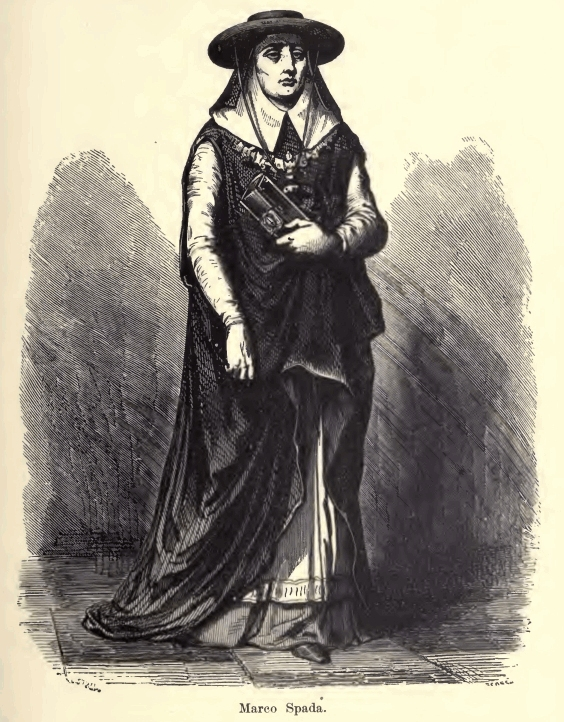
\includegraphics[width=\textwidth]{0239m.jpg}
\end{figure}

“It is time now to proceed to the last part of the speculation. The
pope heaped attentions upon Rospigliosi and Spada, conferred upon them
the insignia of the cardinalate, and induced them to arrange their
affairs and take up their residence at Rome. Then the pope and Cæsar
Borgia invited the two cardinals to dinner. This was a matter of
dispute between the Holy Father and his son. Cæsar thought they could
make use of one of the means which he always had ready for his friends,
that is to say, in the first place, the famous key which was given to
certain persons with the request that they go and open a designated
cupboard. This key was furnished with a small iron point,—a negligence
on the part of the locksmith. When this was pressed to effect the
opening of the cupboard, of which the lock was difficult, the person
was pricked by this small point, and died next day. Then there was the
ring with the lion’s head, which Cæsar wore when he wanted to greet his
friends with a clasp of the hand. The lion bit the hand thus favored,
and at the end of twenty-four hours, the bite was mortal.

“Cæsar proposed to his father, that they should either ask the
cardinals to open the cupboard, or shake hands with them; but Alexander
VI. replied: ‘Now as to the worthy cardinals, Spada and Rospigliosi,
let us ask both of them to dinner, something tells me that we shall get
that money back. Besides, you forget, Cæsar, an indigestion declares
itself immediately, while a prick or a bite occasions a delay of a day
or two.’ Cæsar gave way before such cogent reasoning, and the cardinals
were consequently invited to dinner.

“The table was laid in a vineyard belonging to the pope, near San
Pierdarena, a charming retreat which the cardinals knew very well by
report. Rospigliosi, quite set up with his new dignities, went with a
good appetite and his most ingratiating manner. Spada, a prudent man,
and greatly attached to his only nephew, a young captain of the highest
promise, took paper and pen, and made his will. He then sent word to
his nephew to wait for him near the vineyard; but it appeared the
servant did not find him.

“Spada knew what these invitations meant; since Christianity, so
eminently civilizing, had made progress in Rome, it was no longer a
centurion who came from the tyrant with a message, ‘Cæsar wills that
you die.’ but it was a legate \textit{à latere}, who came with a smile on his
lips to say from the pope, ‘His holiness requests you to dine with
him.’

“Spada set out about two o’clock to San Pierdarena. The pope awaited
him. The first sight that attracted the eyes of Spada was that of his
nephew, in full costume, and Cæsar Borgia paying him most marked
attentions. Spada turned pale, as Cæsar looked at him with an ironical
air, which proved that he had anticipated all, and that the snare was
well spread.

“They began dinner and Spada was only able to inquire of his nephew if
he had received his message. The nephew replied no; perfectly
comprehending the meaning of the question. It was too late, for he had
already drunk a glass of excellent wine, placed for him expressly by
the pope’s butler. Spada at the same moment saw another bottle approach
him, which he was pressed to taste. An hour afterwards a physician
declared they were both poisoned through eating mushrooms. Spada died
on the threshold of the vineyard; the nephew expired at his own door,
making signs which his wife could not comprehend.

“Then Cæsar and the pope hastened to lay hands on the heritage, under
pretense of seeking for the papers of the dead man. But the inheritance
consisted in this only, a scrap of paper on which Spada had written:—‘I
bequeath to my beloved nephew my coffers, my books, and, amongst
others, my breviary with the gold corners, which I beg he will preserve
in remembrance of his affectionate uncle.’

“The heirs sought everywhere, admired the breviary, laid hands on the
furniture, and were greatly astonished that Spada, the rich man, was
really the most miserable of uncles—no treasures—unless they were those
of science, contained in the library and laboratories. That was all.
Cæsar and his father searched, examined, scrutinized, but found
nothing, or at least very little; not exceeding a few thousand crowns
in plate, and about the same in ready money; but the nephew had time to
say to his wife before he expired: ‘Look well among my uncle’s papers;
there is a will.’

“They sought even more thoroughly than the august heirs had done, but
it was fruitless. There were two palaces and a vineyard behind the
Palatine Hill; but in these days landed property had not much value,
and the two palaces and the vineyard remained to the family since they
were beneath the rapacity of the pope and his son. Months and years
rolled on. Alexander VI. died, poisoned,—you know by what mistake.
Cæsar, poisoned at the same time, escaped by shedding his skin like a
snake; but the new skin was spotted by the poison till it looked like a
tiger’s. Then, compelled to quit Rome, he went and got himself
obscurely killed in a night skirmish, scarcely noticed in history.

“After the pope’s death and his son’s exile, it was supposed that the
Spada family would resume the splendid position they had held before
the cardinal’s time; but this was not the case. The Spadas remained in
doubtful ease, a mystery hung over this dark affair, and the public
rumor was, that Cæsar, a better politician than his father, had carried
off from the pope the fortune of the two cardinals. I say the two,
because Cardinal Rospigliosi, who had not taken any precaution, was
completely despoiled.

“Up to this point,” said Faria, interrupting the thread of his
narrative, “this seems to you very meaningless, no doubt, eh?”

“Oh, my friend,” cried Dantès, “on the contrary, it seems as if I were
reading a most interesting narrative; go on, I beg of you.”

“I will. The family began to get accustomed to their obscurity. Years
rolled on, and amongst the descendants some were soldiers, others
diplomatists; some churchmen, some bankers; some grew rich, and some
were ruined. I come now to the last of the family, whose secretary I
was—the Count of Spada. I had often heard him complain of the
disproportion of his rank with his fortune; and I advised him to invest
all he had in an annuity. He did so, and thus doubled his income. The
celebrated breviary remained in the family, and was in the count’s
possession. It had been handed down from father to son; for the
singular clause of the only will that had been found, had caused it to
be regarded as a genuine relic, preserved in the family with
superstitious veneration. It was an illuminated book, with beautiful
Gothic characters, and so weighty with gold, that a servant always
carried it before the cardinal on days of great solemnity.

“At the sight of papers of all sorts,—titles, contracts, parchments,
which were kept in the archives of the family, all descending from the
poisoned cardinal, I in my turn examined the immense bundles of
documents, like twenty servitors, stewards, secretaries before me; but
in spite of the most exhaustive researches, I found—nothing. Yet I had
read, I had even written a precise history of the Borgia family, for
the sole purpose of assuring myself whether any increase of fortune had
occurred to them on the death of the Cardinal Cæsar Spada; but could
only trace the acquisition of the property of the Cardinal Rospigliosi,
his companion in misfortune.

“I was then almost assured that the inheritance had neither profited
the Borgias nor the family, but had remained unpossessed like the
treasures of the Arabian Nights, which slept in the bosom of the earth
under the eyes of the genie. I searched, ransacked, counted, calculated
a thousand and a thousand times the income and expenditure of the
family for three hundred years. It was useless. I remained in my
ignorance, and the Count of Spada in his poverty.

“My patron died. He had reserved from his annuity his family papers,
his library, composed of five thousand volumes, and his famous
breviary. All these he bequeathed to me, with a thousand Roman crowns,
which he had in ready money, on condition that I would have anniversary
masses said for the repose of his soul, and that I would draw up a
genealogical tree and history of his house. All this I did
scrupulously. Be easy, my dear Edmond, we are near the conclusion.

“In 1807, a month before I was arrested, and a fortnight after the
death of the Count of Spada, on the 25th of December (you will see
presently how the date became fixed in my memory), I was reading, for
the thousandth time, the papers I was arranging, for the palace was
sold to a stranger, and I was going to leave Rome and settle at
Florence, intending to take with me twelve thousand francs I possessed,
my library, and the famous breviary, when, tired with my constant labor
at the same thing, and overcome by a heavy dinner I had eaten, my head
dropped on my hands, and I fell asleep about three o’clock in the
afternoon.

\begin{figure}[ht]
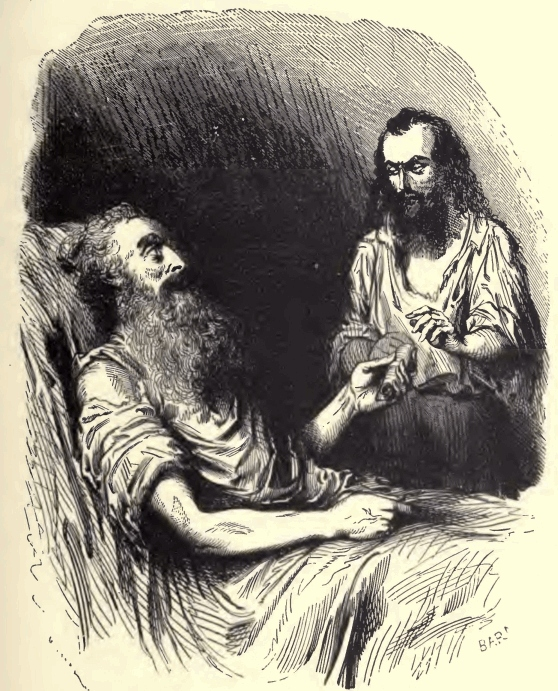
\includegraphics[width=\textwidth]{0243m.jpg}
\end{figure}

“I awoke as the clock was striking six. I raised my head; I was in
utter darkness. I rang for a light, but, as no one came, I determined
to find one for myself. It was indeed but anticipating the simple
manners which I should soon be under the necessity of adopting. I took
a wax-candle in one hand, and with the other groped about for a piece
of paper (my match-box being empty), with which I proposed to get a
light from the small flame still playing on the embers. Fearing,
however, to make use of any valuable piece of paper, I hesitated for a
moment, then recollected that I had seen in the famous breviary, which
was on the table beside me, an old paper quite yellow with age, and
which had served as a marker for centuries, kept there by the request
of the heirs. I felt for it, found it, twisted it up together, and
putting it into the expiring flame, set light to it.

“But beneath my fingers, as if by magic, in proportion as the fire
ascended, I saw yellowish characters appear on the paper. I grasped it
in my hand, put out the flame as quickly as I could, lighted my taper
in the fire itself, and opened the crumpled paper with inexpressible
emotion, recognizing, when I had done so, that these characters had
been traced in mysterious and sympathetic ink, only appearing when
exposed to the fire; nearly one-third of the paper had been consumed by
the flame. It was that paper you read this morning; read it again,
Dantès, and then I will complete for you the incomplete words and
unconnected sense.”

Faria, with an air of triumph, offered the paper to Dantès, who this
time read the following words, traced with an ink of a reddish color
resembling rust:

\vskip \onelineskip

\begin{quote}

{\small“This 25th day of April, 1498, be...

Alexander VI., and fearing that not...

he may desire to become my heir, and re...

and Bentivoglio, who were poisoned,...

my sole heir, that I have bu...

and has visited with me, that is, in...

Island of Monte Cristo, all I poss...

jewels, diamonds, gems; that I alone...

may amount to nearly two mil...

will find on raising the twentieth ro...

creek to the east in a right line. Two open...

in these caves; the treasure is in the furthest a...

which treasure I bequeath and leave en...

as my sole heir.

“25th April, 1498.

“Cæs...}
\end{quote}

\vskip \onelineskip

“And now,” said the abbé, “read this other paper;” and he presented to
Dantès a second leaf with fragments of lines written on it, which
Edmond read as follows:

\vskip \onelineskip

\begin{flushright}
{\small...ing invited to dine by his Holiness

...content with making me pay for my hat,

...serves for me the fate of Cardinals Caprara

...I declare to my nephew, Guido Spada

...ried in a place he knows

...the caves of the small

...essed of ingots, gold, money,

...know of the existence of this treasure, which

...lions of Roman crowns, and which he

...ck from the small

...ings have been made

...ngle in the second;

...tire to him

...ar † Spada.”}
\end{flushright}

\vskip \onelineskip

Faria followed him with an excited look.

“And now,” he said, when he saw that Dantès had read the last line,
“put the two fragments together, and judge for yourself.” Dantès
obeyed, and the conjointed pieces gave the following:

\begin{figure}[h]
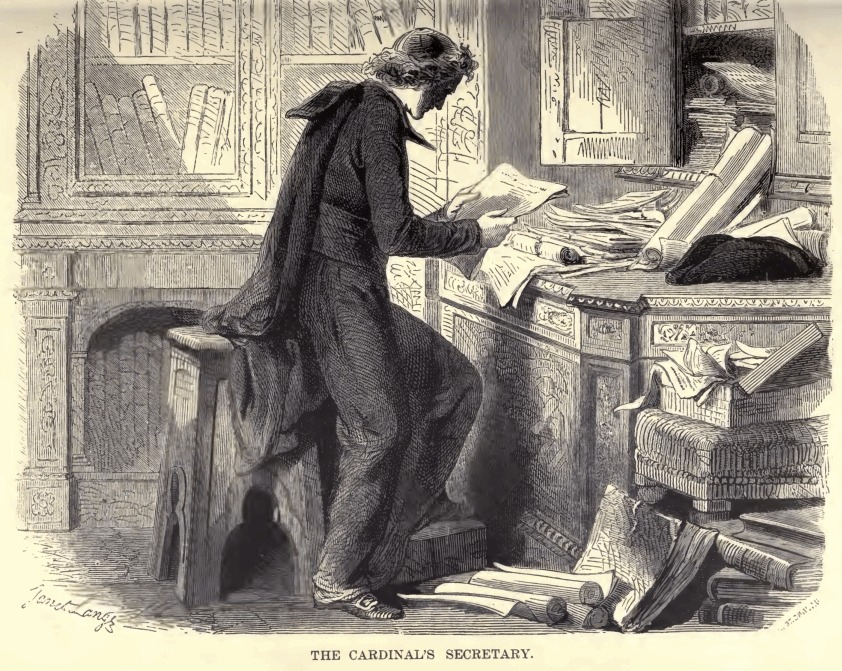
\includegraphics[width=\textwidth]{0245m.jpg}
\end{figure}

“This 25th day of April, 1498, be...ing invited to dine by his Holiness
Alexander VI., and fearing that not...content with making me pay for my
hat, he may desire to become my heir, and re...serves for me the fate
of Cardinals Caprara and Bentivoglio, who were poisoned,...I declare to
my nephew, Guido Spada, my sole heir, that I have bu...ried in a place
he knows and has visited with me, that is, in...the caves of the small
Island of Monte Cristo, all I poss...essed of ingots, gold, money,
jewels, diamonds, gems; that I alone...know of the existence of this
treasure, which may amount to nearly two mil...lions of Roman crowns,
and which he will find on raising the twentieth ro...ck from the small
creek to the east in a right line. Two open...ings have been made in
these caves; the treasure is in the furthest a...ngle in the second;
which treasure I bequeath and leave en...tire to him as my sole heir.
“25th April, 1498. “Cæs...ar † Spada.”

“Well, do you comprehend now?” inquired Faria.

“It is the declaration of Cardinal Spada, and the will so long sought
for,” replied Edmond, still incredulous.

“Yes; a thousand times, yes!”

“And who completed it as it now is?”

“I did. Aided by the remaining fragment, I guessed the rest; measuring
the length of the lines by those of the paper, and divining the hidden
meaning by means of what was in part revealed, as we are guided in a
cavern by the small ray of light above us.”

“And what did you do when you arrived at this conclusion?”

“I resolved to set out, and did set out at that very instant, carrying
with me the beginning of my great work, the unity of the Italian
kingdom; but for some time the imperial police (who at this period,
quite contrary to what Napoleon desired so soon as he had a son born to
him, wished for a partition of provinces) had their eyes on me; and my
hasty departure, the cause of which they were unable to guess, having
aroused their suspicions, I was arrested at the very moment I was
leaving Piombino.

“Now,” continued Faria, addressing Dantès with an almost paternal
expression, “now, my dear fellow, you know as much as I do myself. If
we ever escape together, half this treasure is yours; if I die here,
and you escape alone, the whole belongs to you.”

“But,” inquired Dantès hesitating, “has this treasure no more
legitimate possessor in the world than ourselves?”

“No, no, be easy on that score; the family is extinct. The last Count
of Spada, moreover, made me his heir, bequeathing to me this symbolic
breviary, he bequeathed to me all it contained; no, no, make your mind
satisfied on that point. If we lay hands on this fortune, we may enjoy
it without remorse.”

“And you say this treasure amounts to——”

“Two millions of Roman crowns; nearly thirteen millions of our money.”\footnote[2]{\$2,600,000
in 1894.}

“Impossible!” said Dantès, staggered at the enormous amount.

“Impossible? and why?” asked the old man. “The Spada family was one of
the oldest and most powerful families of the fifteenth century; and in
those times, when other opportunities for investment were wanting, such
accumulations of gold and jewels were by no means rare; there are at
this day Roman families perishing of hunger, though possessed of nearly
a million in diamonds and jewels, handed down by entail, and which they
cannot touch.”

Edmond thought he was in a dream—he wavered between incredulity and
joy.

“I have only kept this secret so long from you,” continued Faria, “that
I might test your character, and then surprise you. Had we escaped
before my attack of catalepsy, I should have conducted you to Monte
Cristo; now,” he added, with a sigh, “it is you who will conduct me
thither. Well, Dantès, you do not thank me?”

“This treasure belongs to you, my dear friend,” replied Dantès, “and to
you only. I have no right to it. I am no relation of yours.”

“You are my son, Dantès,” exclaimed the old man. “You are the child of
my captivity. My profession condemns me to celibacy. God has sent you
to me to console, at one and the same time, the man who could not be a
father, and the prisoner who could not get free.”

And Faria extended the arm of which alone the use remained to him to
the young man, who threw himself upon his neck and wept.

\printpagenotes*
\chapter{TESTIMONY OF EARLY BRETHREN}

THE Tenth Article of Faith reads as follows:

"We believe in the literal gathering of Israel and in the restoration of the Ten Tribes; that
Zion will be built upon this [the American] continent; that Christ will reign personally upon
the earth; and, that the earth will be renewed and receive its paradisiacal glory."

We are also taught that we are living in the "Dispensation of the Fulness of Times." This is
the dispensation into which all other dispensations flow. It is spoken of in the scriptures as
"the times of restitution of all things, which God hath spoken by the mouth of all his holy
prophets since the world began." 1 If the earth is to be renewed, to what is it to be renewed?
It must be to some condition which prevailed in the beginning when the Lord pronounced it
"good." Isaiah, in the 65th chapter of his book gives us the story of what this restoration will
be. Likewise in the Doctrine and Covenants, Section 101, verses 23 to 30, we are given a
similar account, and in the same book, Section 133, the Lord reveals in some detail other
things pertaining to this restoration. This work of restoration commenced many years ago,
when the Lord prepared for the restoration of the Church in this dispensation, and received its
impetus when the Lord commenced his "marvelous work and a wonder." 2

We learn in Section 133, that the Ten Tribes are to come to the children of Ephraim to
receive their blessings and be restored; the Lamb shall come and stand on Mt. Zion, and on
the Mt. of Olives and "utter his voice out of Zion, and he shall speak from Jerusalem, and his
voice shall be heard among all people." His voice shall break down the mountains, the "great
deep" shall be driven \textit{back} into the North countries, and the islands shall become one land
and Jerusalem and Zion shall be turned back to their own place, "and the earth shall be like as
it was in the days before it was divided. And the Lord, even the Savior, shall stand in the
midst of his people, and shall reign over all flesh."

Some of our brethren who lived in the days of the Prophet Joseph Smith have written
interesting accounts of this condition which was in the beginning and what it will be like in
the restoration. First we will present parts of the story as related by Elder Parley P. Pratt, in
his \textit{Voice of Warning} and as it is re-published by John Taylor, in his \textit{The Government of God.}
President Taylor introduces the quotation from Elder Parley P. Pratt's writings with the
following sentence:

Now, restoration signifies a bringing back, and must refer to something which existed before;
for if it did not exist before, it could not be restored. I cannot describe this better than Parley
P. Pratt has done in his \textit{Voice of Warning}, and shall therefore make the following extract:—. .
.

Now, we can never understand precisely what is meant by restoration, unless we understand
what is lost or taken away; for instance, when we offer to restore any thing to a man, it is as
much as to say he once possessed it, but had lost it, and we propose to replace or put him in
possession of that which he once had; therefore, when a prophet speaks of the restoration of
\textit{all things}, he means \textit{all things} have undergone a change, and are to be again restored to their
primitive order even as they first existed.

First, then, it becomes necessary for us to take a view of creation as it rolled in purity from
the hand of its Creator; and if we can discover the true state in which it then existed, and
understand the changes that have taken place since, then we shall be able to understand what
is to be restored; and thus our minds being prepared, we shall be looking for the very things
which will come, and shall be in no danger of lifting our puny arm, in ignorance, to oppose
the things of God.

First, then, we will take a view of the earth, as to its surface, local situation, and productions.

When God had created the heavens and the earth, and separated the light from the darkness,
his next command was to the waters, Gen. 1:9—And God said, "Let the waters under the
heaven be gathered together into \textit{one place}, and let the dry land appear: and it was so!" From
this we learn a marvelous fact, which very few ever realized or believed in this benighted
age; we learn that the waters, which are now divided into oceans, seas, and lakes, were then
all gathered together, into one vast ocean; and, consequently, that the land, which is now torn
asunder, and divided into continents and islands, almost innumerable, was then \textit{one} vast
continent or body, \textit{not} separated as it is now.

Second, we hear the Lord God pronounce the earth, as well as every thing else, \textit{very good.}
From this we learn that there were neither deserts, barren places, stagnant swamps, rough,
broken, ragged hills, nor vast mountains covered with eternal snows; and no part of it was
located in the frigid zones, so as to render its climate dreary and unproductive, subject to
eternal frost, or everlasting chains of ice,—

Where no sweet flowers the dreary landscape cheer, Nor plenteous harvests crown the
passing year;

but the whole earth was probably one vast plain, or interspersed with gently rising hills, and
sloping vales, well calculated for cultivation; while its climate was delightfully varied with
the moderate changes of heat and cold, of wet and dry, which only tended to crown the
varied year, with the greater variety of productions, all for the good of man, animal, fowl, or
creeping thing; while from the flowery plain, or spicy grove, sweet odors were wafted on
every breeze; and all the vast creation of animated beings breathed naught but health, peace,
and joy.

Next, we learn from Genesis 1:29-30, "And God said, Behold, I have given you every herb
bearing seed, which is upon the face of all the earth, and every tree, in which is the fruit of a
tree, yielding seed; to you it shall be for meat. And to every beast of the earth, and to every
fowl of the air, and to every thing that creepeth upon the earth, wherein there is life, I have
given every green herb for meat: and it was so." From these verses we learn that the earth
yielded neither noxious weeds nor poisonous plants, nor useless thorns and thistles; indeed,
everything that grew was just calculated for the food of man, beast, fowl, and creeping thing;
and their food was all vegetable; flesh and blood were never sacrificed to glut their souls, or
gratify their appetites; the beasts of the earth were all in perfect harmony with each other; the
lion ate straw like the ox—the wolf dwelt with the lamb—the leopard lay down with the
kid—the cow and bear fed together, in the same pasture . . . in perfect security, under the
shade of the same trees; all was peace and harmony, and nothing to hurt nor disturb, in all the
holy mountain.

And to crown the whole, we behold man created in the image of God, and exalted in dignity
and power, having dominion over all the vast creation of animated beings, which swarmed
through the earth, while at the same time, he inhabits a beautiful and well-watered garden, in
the midst of which stood the tree of life, to which he had free access; while he stood in the
presence of his Maker, conversed with him face to face, and gazed upon his glory, without a
dimming veil between. O reader, contemplate, for a moment, this beautiful creation, clothed
with peace and plenty; the earth teeming with harmless animals, rejoicing over all the plain,
the air swarming with delightful birds, whose never ceasing notes filled the air with varied
melody; and all in subjection to their rightful sovereign who rejoiced over them; while, in a
delightful garden—the capital of creation,—man was seated on the throne of his vast empire,
swaying his scepter over all the earth, with undisputed right; while legions of angels
encamped round about him, and joined their glad voices in grateful songs of praise, and
shouts of joy; neither a sign nor a groan was heard, throughout the vast expanse; neither was
there sorrow, tears, pain, weeping, sickness, nor death; neither contention, wars, nor
bloodshed; but peace crowned the seasons as they rolled, and life, joy, and love reigned over
all his works. But, O! how changed the scene.

It now becomes my painful duty, to trace some of the important changes, which have taken
place, and the causes which have conspired to reduce the earth and its inhabitants to their
present state.

First, man fell from his standing before God, by giving heed to temptation; and this fall
affected the whole creation, as well as man, and caused various changes to take place; he was
banished from the presence of his Creator, and a veil was drawn between them, and he was
driven from the garden of Eden, to till the earth, which was cursed for man's sake, and should
bring forth thorns and thistles; and in the sweat of his face should earn his bread, and in
sorrow eat of it, all the days of his life, and finally return to dust. But as to Eve, her curse was
a great multiplicity of sorrow and conception; and between her and the seed of the serpent,
there was to be a constant enmity; it should bruise the serpent's head, and the serpent should
bruise his heel.

Now, reader, contemplate the change. This scene, which was so beautiful a little while
before, had now become the abode of sorrow and toil, of death and mourning; the earth
groaned with its production of accursed thorns and thistles; man and beast at enmity; the
serpent slily creeping away, fearing lest his head should get the deadly bruise; and man
starting amid the thorny path, in fear, lest the serpent's fangs should pierce his heel; while the
lamb yields his blood upon the smoking altar. Soon man begins to persecute, hate, and
murder his fellow; until at length the earth is filled with violence; all flesh becomes corrupt,
the powers of darkness prevail; and it repented Noah that God had made man, and it grieved
him at his heart, because the Lord should come out in vengeance, and cleanse the earth by
water.

How far the flood may have contributed, to produce the various changes, as to the division of
the earth into broken fragments, islands and continents, mountains and valleys, we have not
been informed; the change must have been considerable. But after the flood, in the days of
Peleg, the earth was divided.—See Gen. 10:25,—a short history, to be sure, of so great anevent; but still it will account for the mighty revolution, which rolled the sea from its own
place in the north, and brought it to interpose between different portions of the earth, which
were thus parted asunder, and moved into something near their present form; this, together
with the earthquakes, revolutions, and commotions which have since taken place, have all
contributed to reduce the face of the earth to its present state; while the great curses which
have fallen upon different portions, because of the wickedness of men, will account for the
the stagnant swamps, the sunken lakes, the dead seas, and great deserts.

Then speaking of the restoration we have a continuation as follows:

Thus you see, every mountain being laid low, and every valley exalted, and the rough places
being made plain, and the crooked straight, that these mighty revolutions will begin to restore
the face of the earth to its former beauty. But all this done, we have not yet gone through our
restoration; there are many more great things to be done, in order to restore all things. . . .

Thus, having cleansed the earth, and glorified it with the knowledge of God, as the waters
cover the sea, and having poured out his Spirit upon all flesh, both men and beast becoming
perfectly harmless, as they were in the beginning, and feeding on vegetable food only, while
nothing is left to hurt or destroy in all the vast creation, the prophets then proceed to give us
many glorious descriptions of the enjoyment of its inhabitants. "They shall build houses and
inhabit them; they shall plant vineyards, and drink the wine of them; they shall plant gardens
and eat the fruit of them; they shall not build and another inhabit; they shall not plant and
another eat; for as the days of a tree are the days of my people, and mine elect shall enjoy the
work of their hands. They shall not labor in vain, nor bring forth in trouble; for they are the
seed of the blessed of the Lord, and their offspring with them; and it shall come to pass, that
before they call I will answer, and while they are yet speaking I will hear." In this happy state
of existence it seems that all people will live to the full age of a tree, and this too without
pain or sorrow, and whatsoever they ask will be immediately answered, and even all their
wants will be anticipated. Of course, then, none of them will sleep in the dust, for they will
prefer to be translated; that is, changed in the twinkling of an eye, from mortal to immortal;
after which they will continue to reign with Jesus on the earth.

A great council will then be held to adjust the affairs of the world, from the commencement,
over which Father Adam will preside as head and representative of the human family. There
have been, in different ages of the world, communications opened between the heavens and
the earth. (\textit{Voice of Warning and Government of God}, pages 106-115.)

TESTIMONY OF ORSON PRATT

At the funeral of Caroline Grant Smith, wife of William B. Smith, in Nauvoo, May 24, 1845,
Elder Orson Pratt gave the following in his discourse:

In the morning of creation all things were pronounced good by the Creator, as they rolled
into organized existence unsullied and without a curse. Man, the last and noblest of God's
creations, was placed in the garden of Eden, being governed by laws and restricted by
commandments, not being subject to sickness, disease, or death. Adam was placed upon the
earth an immortal being. He was placed in the garden to dress, beautify and adorn it, and to
hold the supremacy of power over all the things of God's creation.

Instead of our first parents eating animal food, they subsisted upon herbs and the fruits of the
earth, which were originally designed for the food of man, and had they not transgressed they
would have both been living upon the earth at the present day, as fair, as healthy, as beautiful
and as free from sickness and death, as they were previous to the transgression. What was
that transgression? it was violating a single commandment of God, and disregarding the
counsel of those immortal beings who stood above them in authority. . . . His was a simple
commandment; but the violation of it subjected Adam to the fall from his exalted station in
the favor of God. Consequently a curse was placed upon all created things, and in the
posterity of Adam were sown the seeds of dissolution. . . . That transgression subjected him
to a curse and that was a fall from a state of immortality to that of mortality; consequently
you see that it was through his agency that death entered the world. (\textit{Times and Seasons}, Vol.
6, pp. 918-919.)

August 29, 1852, the First Presidency asked Orson Pratt to give a discourse on marriage. In
this discourse Elder Pratt said:

The Lord himself solemnized the first marriage pertaining to this globe, and pertaining to
flesh and bones here upon this earth. I do not say pertaining to mortality; for when the first
marriage was celebrated, no mortality was here. The first marriage that we have any account
of, was between two immortal beings—old father Adam and old mother Eve; they were
immortal beings: death had no dominion nor power over them; and they were capable of
enduring forever and ever in their organization. . . .

What would you consider, my hearers, if a marriage was to be celebrated between beings not
subject to death? Would you consider them joined together for a certain number of years, and
that then all their covenants were to cease for ever, and the marriage contract to be dissolved?
Would it look reasonable and consistent? Every heart would say that the work of God is
perfect in and of itself, and inasmuch as sin had not brought imperfection upon the globe,
what God joined together could not be dissolved, and destroyed and torn asunder by any
power beneath the celestial world, consequently it was eternal; the sealing of the great
Jehovah upon Adam and Eve was eternal in its nature. (\textit{Journal of Discourses} Vol. 1, p. 58.)

Again, July 25, 1852, Elder Orson Pratt preached a wonderful discourse, designated as "A
funeral sermon of all Saints and Sinners; also of the heavens and the Earth." This entire
discourse which is printed in the Millennial Star and other publications, should be read by
every member of the Church. It cannot be produced here in its fulness, but the following
taken from it has to do with the subject of Adam and the fall.

I will take a text, which you will find recorded in the 51st chapter of the prophecy of Isaiah,
and the sixth verse: "Lift up your eyes to the heavens, and look upon the earth beneath: for
the heavens shall vanish away like smoke, and the earth shall wax old like a garment, and
they that dwell therein shall die in like manner: but my salvation shall be forever, and my
righteousness shall not be abolished!"

All things with which we are acquainted, pertaining to this earth of ours, are subject to
change; not only man, so far as his temporal body is concerned, but the beasts of the field,
the fowls of the air, the fishes of the sea, and every living thing with which we are
acquainted—all are subject to pain and distress, and finally die and pass away; death seems
to have universal dominion in our creation. It certainly is a curious world; it certainly does
not look like a world constructed in such manner as to produce eternal happiness; and it
would be very far from the truth, I think, for any being at the present time to pronounce it
very good; everything seems to show us that goodness, in a great degree, has fled from this
creation. If we partake of the elements, death is there in all its forms and varieties; and when
we desire to rejoice, sorrow is there, mingling itself in every cup; and woe, and
wretchedness, and misery, seem to be our present doom.

There is something, however, in man, that is constantly reaching forward after happiness,
after pleasure, after something to satisfy the longing desire that dwells within his bosom.
Why is it that we have such a desire? And why is it that it is not satisfied? Why is it that this
creation is so constructed? And why is it that death reigns universally over all living earthly
beings? Did the great Author of creation construct this little globe of ours subject to all these
changes, which are calculated to produce sorrow and death among the beings that inhabit it?
Was this the original condition of our creation? I answer, no; it was not so constructed. But
how was it made in the beginning? All things that were made pertaining to this earth were
pronounced "very good." Where there is pain, where there is sickness, where there is sorrow,
and where there is death, this saying can not be understood in its literal sense; things cannot
be very good where something very evil reigns and has universal dominion.

We are, therefore, constrained to believe, that in the first formation of our globe, as far as the
Mosaic history gives us the information, everything was perfect in its formation; that there
was nothing in the air, or in the waters or in the solid elements that was calculated to produce
misery, wretchedness, unhappiness, or death, in the way that it was then organized; not but
what the same elements, organized a little differently, would produce all these effects; but as
it was then constructed, we must admit that every particle of air, of water, and earth, was so
organized as to be capable of diffusing life and immortality through all the varied species of
animated existence—immortality reigned in every department of creation; hence it was
pronounced "very good."

When the Lord made the fowls of the air, and the fishes of the sea, to people the atmospheric
heavens, or the watery elements, these fowls and fishes were so constructed in their nature as
to be capable of eternal existence. To imagine anything different from this, would be to
suppose the Almighty to form that which was calculated to produce wretchedness and
misery. What says the Psalmist David upon the subject? He says that all the works of the
Lord shall endure forever. Did not the Lord make the fish? Did he not make the fowls of the
heavens? Yes. Did he not make the beasts of the field, and the creeping things, and the
insects? Yes. Do they endure forever? They apparently do not; and yet David says all his
works are constructed upon that principle. Is this a contradiction? No. God has given some
other particulars in relation to these works. He has permitted the destroyer to visit them, who
has usurped a certain dominion and authority, carrying desolation and ruin on every hand; the
perfections of the original organizations have ceased. But will the Lord for ever permit these
destructions to reign? No. His power exists, and the power of the destroyer exists. His power
exists, and the power of death exists; but his power exceeds all other powers; and
consequently wherever a usurper comes in and lays waste any of his works, he will repair
these wastes, build up the old ruins, and make all things new: Even the fish of the sea, and
the fowls of the heavens, and the beasts of the earth, must yet, in order to carry out the
designs of the Almighty, be so constructed as to be capable of eternal existence.

It would be interesting to know something about the situation of things when they were first
formed, and how this destroyer happened to make inroads upon this fair creation; what the
causes were, and why it was permitted.

Man, when he was first placed upon this earth, was an immortal being, capable of eternal
endurance; his flesh and bones, as well as his spirit, were immortal and eternal in their
nature; and it was just so with all the inferior creation—the lion, the leopard, the kid, and the
cow; it was so with the feathered tribes of creation, as well as those that swim in the vast
ocean of waters; all were immortal and eternal in their nature; and the earth itself, as a living
being, was immortal and eternal in its nature. What! is the earth alive too? If it were not, how
could the words of our text be fulfilled, where it speaks of the earth's dying? How can that
die that has no life? "Lift up your eyes to the heavens above, say the Lord, and look upon the
earth beneath: for the heavens shall vanish away like smoke, and the earth shall wax old like
a garment, and they that dwell therein shall die in like manner." What! the earth and the
heavens to die? Yes, the material heavens and the earth must all undergo this change which
we call death; and if so, the earth must be alive as well as we. The earth was so constructed
that it was capable of existing as a living being to all eternity, with all the swarms of animals,
fowls, and fishes that were first placed upon the face thereof. But how can it be proved that
man was an immortal being? We will refer you to what the Apostle Paul has written upon
this subject: he says that by one man came death; and he tells us how it came: It was by the
transgression of one individual that death was introduced here. But did transgression bring in
all these diseases and this sorrow, this misery and wretchedness, over the whole face of this
creation? Is it by the transgression of one person that the very heavens are to vanish away as
smoke, and the earth is to wax old like a garment? Yes, it is by the transgression of one; and
if it had not been for his transgression, the earth never would have been subject to death.
Why? Because the works of the Lord are so constructed as to exist for ever; and if death had
come in without a cause, and destroyed the earth, and laid waste the material heavens, and
produced a general and utter overthrow and ruin in this fair creation, then the works of the
Lord would have ceased to endure according to the promise, being imperfect in their
construction, and consequently not very good.

But what was the sin, and what was the nature of it? I will tell you what it was; it was merely
the partaking of a certain kind of fruit. But, says one, "I should think there is no harm in
eating fruit." There would not be unless God gave a command upon the subject. There are
things in nature that would be evil without a commandment: If there were no commandment,
it would be evil for you to murder an innocent being, and your own conscience would tell
you it was an evil thing. It is an evil for any individual to injure another, or to infringe upon
the rights of another, independent of any revealed law; for the savage, or that being who has
never heard of the written laws of heaven—who has never heard of the revealed laws of
God—with regard to these principles—as well as the Saint, knows that it is an evil to infringe
upon the rights of another; the very nature of the thing shows that it is an evil; but not so in
regard to many other things that are evil; which are only made evil by commandment.

For instance, here is the Sabbath day; a person who never heard the revealed law of God
upon the subject, never could conceive that it was an evil to work on the Sabbath day; he
would consider it just as right to work on the first day of the week, as on the seventh; he
would perceive nothing in the nature of the thing by which he could distinguish it to be an
evil. So with regard to eating certain fruit, it was the commandment of the Great God that
made it an evil. He said to Adam and Eve, "Here are all the fruits of the garden; you may eat
of them freely except this one tree that stands in the midst of the garden; now beware for in
the day you eat thereof you shall surely die." Don't we perceive that the commandment made
this an evil? Had it not been for this commandment, Adam would have walked forth and
freely partaken of every tree, without any remorse of conscience; just as the savage, who
never had heard the revealed will of God, would work on the Sabbath, the same as on any
other day, and have no conscience about the matter. But when a man murders, he knows it to
be an injury, and he has a conscience about it, though he never heard of God; and so with
thousands of evils. But why did the Lord place man under these peculiar circumstances?
Why did he not withhold the commandment, if the partaking of the fruit, after the
commandment was given, was sin? Why should there have been a commandment upon the
subject at all, inasmuch as there was no evil in the nature of the thing to be perceived or
understood? The Lord had a purpose in view; though he constructed this fair creation, as we
have told you, subject to immortality, and capable of eternal endurance, and though he had
constructed men capable of living forever, yet he had an object in view in regard to that man,
and the creation he inhabited. What was the object? And when shall this object be
accomplished?

Why, the Lord wanted this intelligent being called man, to prove himself; inasmuch as he
was an agent. He desired that he should show himself approved before his Creator.

How could this be done without a commandment? Can you devise any possible means? Is
there any person in this congregation having wisdom sufficient to devise any means by which
an intelligent being can show himself approved before a superior intelligence, unless it be by
administering to that man certain laws to be kept? No. Without law, without commandment
or rule, there could be no possible way of showing his integrity; it could not be said that he
would keep all the laws that govern superior orders of beings, unless he had been placed in a
position to be tried, and thus proved whether he would keep them or not. Then it was wisdom
to try the man and the woman, so the Lord gave them this commandment; if he had not
intended the man should be tried by this commandment, he never would have planted that
tree. He never would have placed it in the midst of the garden. Now the very fact that he
planted it where the man could have easy access to it, shows that he intended man should be
tried by it, and thus prove whether he would keep his commandments or not. The penalty of
disobedience to this law was death.

But could he not give a commandment, without affixing a penalty? He could not; it would be
folly, even worse than folly, for God to give a law to an intelligent being, without affixing a
penalty to it if it were broken. Why? Because all intelligent beings would discard the very
idea of a law being given, which might be broken at pleasure, without the individuals
breaking it being punished for their transgression. They would say—"Where is the principle
of justice in the giver of the law? It is not here: we do not reverence him nor his law; justice
does not have an existence in his bosom. He does not regard his own laws, for he suffers
them to be broken with impunity, and trampled under foot by those whom he has made;
therefore we care not for him or his laws; nor his pretended justice. We will rebel against it.
Where would have been the use of it if there had been no penalty affixed?

But what is the nature of this penalty? It was wisely ordained to be of such a nature as to
instruct man. Penalties inflicted upon human beings here, by governors, kings, or rulers, are
generally of such a nature as to benefit them.

Adam was appointed lord of this creation; a great governor, swaying the scepter of power
over the whole earth. When the governor, the person who was placed to reign over this fair
creation, had transgressed, all in his dominion had to feel the effects of it, the same as a
father or a mother, who transgress certain laws, frequently transmit the effects thereof to the
latest generations.

How often do we see certain diseases becoming hereditary, being handed down from father
to son for generations? Why? Because in the first instance there was a transgression, and the
children partook of the effects of it. And what was the fullest extent of the penalty of Adam's
transgression? I will tell you—it was death. The death of the immortal tabernacle—of the
tabernacle where the seeds of death had not been, that was wisely framed, and pronounced
very good; the seeds of death were introduced into it. How and in what manner? Some say
there was something in the nature of the fruit that introduced mortality. Be this as it may, one
thing is certain, death entered into the system; it came there by some means, and sin was the
main spring by which this monster was introduced. If there had been no sin, our father Adam
would at this day have been in the garden of Eden, as bright and as blooming, as fresh and as
fair, as ever, together with his lovely consort Eve, dwelling in all the beauty of youth.

By one man came death—the death of the body. What becomes of the spirit when the body
dies? Will it be perfectly happy? Would old father Adam's spirit have gone back into the
presence of God, and dwelt there eternally, enjoying all the felicities and glories of heaven,
after his body had died? No; for the penalty of that transgression was not limited to the body
alone. When he sinned, it was with both the body and the spirit that he sinned. It was not only
the body that ate of the fruit, but the spirit gave the will to eat; the spirit sinned therefore as
well as the body; they were agreed in partaking of that fruit. Was not the spirit to suffer then
as well as the body? Yes. How long? To all ages of eternity, without any end, while the body
was to return back to its mother earth, and there slumber to all eternity. That was the effect of
the fall, leaving out the plan of redemption; so that, if there had been no plan of redemption
prepared from before the foundation of the world, man would have been subject to an eternal
dissolution of the body and spirit—the one to lie mingling with its mother earth, to all ages of
eternity, and the other to be subject, throughout all future duration, to the power that deceived
him, and led them astray; to be completely miserable, or as the Book of Mormon says, "dead
as to things pertaining to righteousness." (\textit{Journal of Discourses}, Vol. 1, pp. 280-284.)

From an epistle by the Prophet to the Elders in Missouri, sent January 22, 1834, the
following is taken:

Though man in his own supposed wisdom would not admit the influence of a power superior
to his own, yet for wise and great purposes, for the good and happiness of his creatures, God
has instructed man to form wise and wholesome laws, since he had departed from him and
refused to be governed by those laws which God had given by his own voice from on high in
the beginning. But notwithstanding the transgression, by which man had cut himself off from
an immediate intercourse with his maker without a Mediator, it appears that the great and
glorious plan of his redemption was previously provided: the sacrifice prepared; the
atonement wrought out in the mind and purpose of God, even in the person of the Son,
through whom man was now to look for acceptance and through whose merits he was now
taught that he alone could find redemption, since the word had been pronounced, Unto dust
thou shalt return.

But that man was not able himself to erect a system, or plan with power sufficient to free him
from a destruction which awaited him is evident from the fact that God, as before remarked,
prepared a sacrifice in the gift of his own Son who should be sent in due time, to prepare a
way, or open a door through which man might enter into the Lord's presence, whence he had
been cast out for disobedience. From time to time these glad tidings were sounded in the ears
of men in different ages of the world down to the time of Messiah's coming. By faith in the
atonement or plan of redemption, Abel offered to God a sacrifice that was accepted, which
was the firstlings of the flock. Cain offered of the fruit of the ground, and was not accepted,
because he could not do it in faith; he could have no faith, or could not exercise faith contrary
to the plan of heaven. It must be shedding of blood of the Only Begotten to atone for man;
for this was the plan of redemption; and without the shedding of blood was no remission; and
as the sacrifice was instituted as a type, by which man was to discern the great Sacrifice
which God had prepared; to offer a sacrifice contrary to that, no faith could be exercised,
because redemption was not purchased in that way, nor the power of atonement instituted
after that order; consequently Cain could have no faith; and whatsoever is not faith is sin.
(\textit{Teachings of the Prophet Joseph Smith}, pp. 57-58.)

\newpage
Footnotes

1. Acts 3:21.

2. D. \& C. Sec. 4.


\printpagenotes*
\chapter{Conversion Of Constantine.}
\section{Part \thesection.}

\textit{The Motives, Progress, And Effects Of The Conversion Of
Constantine. — Legal Establishment And Constitution Of The Christian Or
Catholic Church.}
\vspace{\onelineskip}

The public establishment of Christianity may be considered as one of
those important and domestic revolutions which excite the most lively
curiosity, and afford the most valuable instruction. The victories and
the civil policy of Constantine no longer influence the state of
Europe; but a considerable portion of the globe still retains the
impression which it received from the conversion of that monarch; and
the ecclesiastical institutions of his reign are still connected, by an
indissoluble chain, with the opinions, the passions, and the interests
of the present generation. In the consideration of a subject which may
be examined with impartiality, but cannot be viewed with indifference,
a difficulty immediately arises of a very unexpected nature; that of
ascertaining the real and precise date of the conversion of
Constantine. The eloquent Lactantius, in the midst of his court, seems
impatient\textsuperscript{1} to proclaim to the world the glorious example of the
sovereign of Gaul; who, in the first moments of his reign, acknowledged
and adored the majesty of the true and only God.\textsuperscript{2} The learned Eusebius
has ascribed the faith of Constantine to the miraculous sign which was
displayed in the heavens whilst he meditated and prepared the Italian
expedition.\textsuperscript{3} The historian Zosimus maliciously asserts, that the
emperor had imbrued his hands in the blood of his eldest son, before he
publicly renounced the gods of Rome and of his ancestors.\textsuperscript{4} The
perplexity produced by these discordant authorities is derived from the
behavior of Constantine himself. According to the strictness of
ecclesiastical language, the first of the \textit{Christian} emperors was
unworthy of that name, till the moment of his death; since it was only
during his last illness that he received, as a catechumen, the
imposition of hands,\textsuperscript{5} and was afterwards admitted, by the initiatory
rites of baptism, into the number of the faithful.\textsuperscript{6} The Christianity
of Constantine must be allowed in a much more vague and qualified
sense; and the nicest accuracy is required in tracing the slow and
almost imperceptible gradations by which the monarch declared himself
the protector, and at length the proselyte, of the church. It was an
arduous task to eradicate the habits and prejudices of his education,
to acknowledge the divine power of Christ, and to understand that the
truth of \textit{his} revelation was incompatible with the worship of the
gods. The obstacles which he had probably experienced in his own mind,
instructed him to proceed with caution in the momentous change of a
national religion; and he insensibly discovered his new opinions, as
far as he could enforce them with safety and with effect. During the
whole course of his reign, the stream of Christianity flowed with a
gentle, though accelerated, motion: but its general direction was
sometimes checked, and sometimes diverted, by the accidental
circumstances of the times, and by the prudence, or possibly by the
caprice, of the monarch. His ministers were permitted to signify the
intentions of their master in the various language which was best
adapted to their respective principles;\textsuperscript{7} and he artfully balanced the
hopes and fears of his subjects, by publishing in the same year two
edicts; the first of which enjoined the solemn observance of Sunday,\textsuperscript{8}
and the second directed the regular consultation of the Aruspices.\textsuperscript{9}
While this important revolution yet remained in suspense, the
Christians and the Pagans watched the conduct of their sovereign with
the same anxiety, but with very opposite sentiments. The former were
prompted by every motive of zeal, as well as vanity, to exaggerate the
marks of his favor, and the evidences of his faith. The latter, till
their just apprehensions were changed into despair and resentment,
attempted to conceal from the world, and from themselves, that the gods
of Rome could no longer reckon the emperor in the number of their
votaries. The same passions and prejudices have engaged the partial
writers of the times to connect the public profession of Christianity
with the most glorious or the most ignominious æra of the reign of
Constantine.

\pagenote[1]{The date of the Divine Institutions of Lactantius has been
accurately discussed, difficulties have been started, solutions
proposed, and an expedient imagined of two \textit{original} editions; the
former published during the persecution of Diocletian, the latter under
that of Licinius. See Dufresnoy, Prefat. p. v. Tillemont, Mém.
Ecclesiast. tom. vi. p. 465-470. Lardner’s Credibility, part ii. vol.
vii. p. 78-86. For my own part, I am \textit{almost} convinced that Lactantius
dedicated his Institutions to the sovereign of Gaul, at a time when
Galerius, Maximin, and even Licinius, persecuted the Christians; that
is, between the years 306 and 311.}

\pagenote[2]{Lactant. Divin. Instit. i. l. vii. 27. The first and most
important of these passages is indeed wanting in twenty-eight
manuscripts; but it is found in nineteen. If we weigh the comparative
value of these manuscripts, one of 900 years old, in the king of
France’s library may be alleged in its favor; but the passage is
omitted in the correct manuscript of Bologna, which the P. de
Montfaucon ascribes to the sixth or seventh century (Diarium Italic. p.
489.) The taste of most of the editors (except Isæus; see Lactant.
edit. Dufresnoy, tom. i. p. 596) has felt the genuine style of
Lactantius.}

\pagenote[3]{Euseb. in Vit. Constant. l. i. c. 27-32.}

\pagenote[4]{Zosimus, l. ii. p. 104.}

\pagenote[5]{That rite was \textit{always} used in making a catechumen, (see
Bingham’s Antiquities. l. x. c. i. p. 419. Dom Chardon, Hist. des
Sacramens, tom. i. p. 62,) and Constantine received it for the \textit{first}
time (Euseb. in Vit Constant. l. iv. c. 61) immediately before his
baptism and death. From the connection of these two facts, Valesius (ad
loc. Euseb.) has drawn the conclusion which is reluctantly admitted by
Tillemont, (Hist. des Empereurs, tom. iv. p. 628,) and opposed with
feeble arguments by Mosheim, (p. 968.)}

\pagenote[6]{Euseb. in Vit. Constant. l. iv. c. 61, 62, 63. The legend
of Constantine’s baptism at Rome, thirteen years before his death, was
invented in the eighth century, as a proper motive for his \textit{donation}.
Such has been the gradual progress of knowledge, that a story, of which
Cardinal Baronius (Annual Ecclesiast. A. D. 324, No. 43-49) declared
himself the unblushing advocate, is now feebly supported, even within
the verge of the Vatican. See the Antiquitates Christianæ, tom. ii. p.
232; a work published with six approbations at Rome, in the year 1751
by Father Mamachi, a learned Dominican.}

\pagenote[7]{The quæstor, or secretary, who composed the law of the
Theodosian Code, makes his master say with indifference, “hominibus
supradictæ religionis,” (l. xvi. tit. ii. leg. 1.) The minister of
ecclesiastical affairs was allowed a more devout and respectful style,
[**Greek] the legal, most holy, and Catholic worship.}

\pagenote[8]{Cod. Theodos. l. ii. viii. tit. leg. 1. Cod. Justinian. l.
iii. tit. xii. leg. 3. Constantine styles the Lord’s day \textit{dies solis},
a name which could not offend the ears of his pagan subjects.}

\pagenote[9]{Cod. Theodos. l. xvi. tit. x. leg. l. Godefroy, in the
character of a commentator, endeavors (tom. vi. p. 257) to excuse
Constantine; but the more zealous Baronius (Annal. Eccles. A. D. 321,
No. 17) censures his profane conduct with truth and asperity.}

Whatever symptoms of Christian piety might transpire in the discourses
or actions of Constantine, he persevered till he was near forty years
of age in the practice of the established religion;\textsuperscript{10} and the same
conduct which in the court of Nicomedia might be imputed to his fear,
could be ascribed only to the inclination or policy of the sovereign of
Gaul. His liberality restored and enriched the temples of the gods; the
medals which issued from his Imperial mint are impressed with the
figures and attributes of Jupiter and Apollo, of Mars and Hercules; and
his filial piety increased the council of Olympus by the solemn
apotheosis of his father Constantius.\textsuperscript{11} But the devotion of
Constantine was more peculiarly directed to the genius of the Sun, the
Apollo of Greek and Roman mythology; and he was pleased to be
represented with the symbols of the God of Light and Poetry. The
unerring shafts of that deity, the brightness of his eyes, his laurel
wreath, immortal beauty, and elegant accomplishments, seem to point him
out as the patron of a young hero. The altars of Apollo were crowned
with the votive offerings of Constantine; and the credulous multitude
were taught to believe, that the emperor was permitted to behold with
mortal eyes the visible majesty of their tutelar deity; and that,
either walking or in a vision, he was blessed with the auspicious omens
of a long and victorious reign. The Sun was universally celebrated as
the invincible guide and protector of Constantine; and the Pagans might
reasonably expect that the insulted god would pursue with unrelenting
vengeance the impiety of his ungrateful favorite.\textsuperscript{12}

\pagenote[10]{Theodoret. (l. i. c. 18) seems to insinuate that Helena
gave her son a Christian education; but we may be assured, from the
superior authority of Eusebius, (in Vit. Constant. l. iii. c. 47,) that
she herself was indebted to Constantine for the knowledge of
Christianity.}

\pagenote[11]{See the medals of Constantine in Ducange and Banduri. As
few cities had retained the privilege of coining, almost all the medals
of that age issued from the mint under the sanction of the Imperial
authority.}

\pagenote[12]{The panegyric of Eumenius, (vii. inter Panegyr. Vet.,)
which was pronounced a few months before the Italian war, abounds with
the most unexceptionable evidence of the Pagan superstition of
Constantine, and of his particular veneration for Apollo, or the Sun;
to which Julian alludes.}

As long as Constantine exercised a limited sovereignty over the
provinces of Gaul, his Christian subjects were protected by the
authority, and perhaps by the laws, of a prince, who wisely left to the
gods the care of vindicating their own honor. If we may credit the
assertion of Constantine himself, he had been an indignant spectator of
the savage cruelties which were inflicted, by the hands of Roman
soldiers, on those citizens whose religion was their only crime.\textsuperscript{13} In
the East and in the West, he had seen the different effects of severity
and indulgence; and as the former was rendered still more odious by the
example of Galerius, his implacable enemy, the latter was recommended
to his imitation by the authority and advice of a dying father. The son
of Constantius immediately suspended or repealed the edicts of
persecution, and granted the free exercise of their religious
ceremonies to all those who had already professed themselves members of
the church. They were soon encouraged to depend on the favor as well as
on the justice of their sovereign, who had imbibed a secret and sincere
reverence for the name of Christ, and for the God of the Christians.\textsuperscript{14}

\pagenote[13]{Constantin. Orat. ad Sanctos, c. 25. But it might easily
be shown, that the Greek translator has improved the sense of the Latin
original; and the aged emperor might recollect the persecution of
Diocletian with a more lively abhorrence than he had actually felt to
the days of his youth and Paganism.}

\pagenote[14]{See Euseb. Hist. Eccles. l. viii. 13, l. ix. 9, and in
Vit. Const. l. i. c. 16, 17 Lactant. Divin. Institut. i. l. Cæcilius de
Mort. Persecut. c. 25.}

About five months after the conquest of Italy, the emperor made a
solemn and authentic declaration of his sentiments by the celebrated
edict of Milan, which restored peace to the Catholic church. In the
personal interview of the two western princes, Constantine, by the
ascendant of genius and power, obtained the ready concurrence of his
colleague, Licinius; the union of their names and authority disarmed
the fury of Maximin; and after the death of the tyrant of the East, the
edict of Milan was received as a general and fundamental law of the
Roman world.\textsuperscript{15}

\pagenote[15]{Cæcilius (de Mort. Persecut. c. 48) has preserved the
Latin original; and Eusebius (Hist. Eccles. l. x. c. 5) has given a
Greek translation of this perpetual edict, which refers to some
provisional regulations.}

The wisdom of the emperors provided for the restitution of all the
civil and religious rights of which the Christians had been so unjustly
deprived. It was enacted that the places of worship, and public lands,
which had been confiscated, should be restored to the church, without
dispute, without delay, and without expense; and this severe injunction
was accompanied with a gracious promise, that if any of the purchasers
had paid a fair and adequate price, they should be indemnified from the
Imperial treasury. The salutary regulations which guard the future
tranquillity of the faithful are framed on the principles of enlarged
and equal toleration; and such an equality must have been interpreted
by a recent sect as an advantageous and honorable distinction. The two
emperors proclaim to the world, that they have granted a free and
absolute power to the Christians, and to all others, of following the
religion which each individual thinks proper to prefer, to which he has
addicted his mind, and which he may deem the best adapted to his own
use. They carefully explain every ambiguous word, remove every
exception, and exact from the governors of the provinces a strict
obedience to the true and simple meaning of an edict, which was
designed to establish and secure, without any limitation, the claims of
religious liberty. They condescend to assign two weighty reasons which
have induced them to allow this universal toleration: the humane
intention of consulting the peace and happiness of their people; and
the pious hope, that, by such a conduct, they shall appease and
propitiate \textit{the Deity}, whose seat is in heaven. They gratefully
acknowledge the many signal proofs which they have received of the
divine favor; and they trust that the same Providence will forever
continue to protect the prosperity of the prince and people. From these
vague and indefinite expressions of piety, three suppositions may be
deduced, of a different, but not of an incompatible nature. The mind of
Constantine might fluctuate between the Pagan and the Christian
religions. According to the loose and complying notions of Polytheism,
he might acknowledge the God of the Christians as \textit{one} of the \textit{many}
deities who compose the hierarchy of heaven. Or perhaps he might
embrace the philosophic and pleasing idea, that, notwithstanding the
variety of names, of rites, and of opinions, all the sects, and all the
nations of mankind, are united in the worship of the common Father and
Creator of the universe.\textsuperscript{16}

\pagenote[16]{A panegyric of Constantine, pronounced seven or eight
months after the edict of Milan, (see Gothofred. Chronolog. Legum, p.
7, and Tillemont, Hist. des Empereurs, tom. iv. p. 246,) uses the
following remarkable expression: “Summe rerum sator, cujus tot nomina
sant, quot linguas gentium esse voluisti, quem enim te ipse dici velin,
scire non possumus.” (Panegyr. Vet. ix. 26.) In explaining
Constantine’s progress in the faith, Mosheim (p. 971, \&c.) is
ingenious, subtle, prolix.}

But the counsels of princes are more frequently influenced by views of
temporal advantage, than by considerations of abstract and speculative
truth. The partial and increasing favor of Constantine may naturally be
referred to the esteem which he entertained for the moral character of
the Christians; and to a persuasion, that the propagation of the gospel
would inculcate the practice of private and public virtue. Whatever
latitude an absolute monarch may assume in his own conduct, whatever
indulgence he may claim for his own passions, it is undoubtedly his
interest that all his subjects should respect the natural and civil
obligations of society. But the operation of the wisest laws is
imperfect and precarious. They seldom inspire virtue, they cannot
always restrain vice. Their power is insufficient to prohibit all that
they condemn, nor can they always punish the actions which they
prohibit. The legislators of antiquity had summoned to their aid the
powers of education and of opinion. But every principle which had once
maintained the vigor and purity of Rome and Sparta, was long since
extinguished in a declining and despotic empire. Philosophy still
exercised her temperate sway over the human mind, but the cause of
virtue derived very feeble support from the influence of the Pagan
superstition. Under these discouraging circumstances, a prudent
magistrate might observe with pleasure the progress of a religion which
diffused among the people a pure, benevolent, and universal system of
ethics, adapted to every duty and every condition of life; recommended
as the will and reason of the supreme Deity, and enforced by the
sanction of eternal rewards or punishments. The experience of Greek and
Roman history could not inform the world how far the system of national
manners might be reformed and improved by the precepts of a divine
revelation; and Constantine might listen with some confidence to the
flattering, and indeed reasonable, assurances of Lactantius. The
eloquent apologist seemed firmly to expect, and almost ventured to
promise, \textit{that} the establishment of Christianity would restore the
innocence and felicity of the primitive age; \textit{that} the worship of the
true God would extinguish war and dissension among those who mutually
considered themselves as the children of a common parent; \textit{that} every
impure desire, every angry or selfish passion, would be restrained by
the knowledge of the gospel; and \textit{that} the magistrates might sheath
the sword of justice among a people who would be universally actuated
by the sentiments of truth and piety, of equity and moderation, of
harmony and universal love.\textsuperscript{17}

\pagenote[17]{See the elegant description of Lactantius, (Divin
Institut. v. 8,) who is much more perspicuous and positive than becomes
a discreet prophet.}

The passive and unresisting obedience, which bows under the yoke of
authority, or even of oppression, must have appeared, in the eyes of an
absolute monarch, the most conspicuous and useful of the evangelic
virtues.\textsuperscript{18} The primitive Christians derived the institution of civil
government, not from the consent of the people, but from the decrees of
Heaven. The reigning emperor, though he had usurped the sceptre by
treason and murder, immediately assumed the sacred character of
vicegerent of the Deity. To the Deity alone he was accountable for the
abuse of his power; and his subjects were indissolubly bound, by their
oath of fidelity, to a tyrant, who had violated every law of nature and
society. The humble Christians were sent into the world as sheep among
wolves; and since they were not permitted to employ force even in the
defence of their religion, they should be still more criminal if they
were tempted to shed the blood of their fellow-creatures in disputing
the vain privileges, or the sordid possessions, of this transitory
life. Faithful to the doctrine of the apostle, who in the reign of Nero
had preached the duty of unconditional submission, the Christians of
the three first centuries preserved their conscience pure and innocent
of the guilt of secret conspiracy, or open rebellion. While they
experienced the rigor of persecution, they were never provoked either
to meet their tyrants in the field, or indignantly to withdraw
themselves into some remote and sequestered corner of the globe.\textsuperscript{19} The
Protestants of France, of Germany, and of Britain, who asserted with
such intrepid courage their civil and religious freedom, have been
insulted by the invidious comparison between the conduct of the
primitive and of the reformed Christians.\textsuperscript{20} Perhaps, instead of
censure, some applause may be due to the superior sense and spirit of
our ancestors, who had convinced themselves that religion cannot
abolish the unalienable rights of human nature.\textsuperscript{21} Perhaps the patience
of the primitive church may be ascribed to its weakness, as well as to
its virtue.

A sect of unwarlike plebeians, without leaders, without arms, without
fortifications, must have encountered inevitable destruction in a rash
and fruitless resistance to the master of the Roman legions. But the
Christians, when they deprecated the wrath of Diocletian, or solicited
the favor of Constantine, could allege, with truth and confidence, that
they held the principle of passive obedience, and that, in the space of
three centuries, their conduct had always been conformable to their
principles. They might add, that the throne of the emperors would be
established on a fixed and permanent basis, if all their subjects,
embracing the Christian doctrine, should learn to suffer and to obey.

\pagenote[18]{The political system of the Christians is explained by
Grotius, de Jure Belli et Pacis, l. i. c. 3, 4. Grotius was a
republican and an exile, but the mildness of his temper inclined him to
support the established powers.}

\pagenote[19]{Tertullian. Apolog. c. 32, 34, 35, 36. Tamen nunquam
Albiniani, nec Nigriani vel Cassiani inveniri potuerunt Christiani. Ad
Scapulam, c. 2. If this assertion be strictly true, it excludes the
Christians of that age from all civil and military employments, which
would have compelled them to take an active part in the service of
their respective governors. See Moyle’s Works, vol. ii. p. 349.}

\pagenote[20]{See the artful Bossuet, (Hist. des Variations des Eglises
Protestantes, tom. iii. p. 210-258.) and the malicious Bayle, (tom ii.
p. 820.) I \textit{name} Bayle, for he was certainly the author of the Avis
aux Refugies; consult the Dictionnaire Critique de Chauffepié, tom. i.
part ii. p. 145.}

\pagenote[21]{Buchanan is the earliest, or at least the most
celebrated, of the reformers, who has justified the theory of
resistance. See his Dialogue de Jure Regni apud Scotos, tom. ii. p. 28,
30, edit. fol. Rudiman.}

In the general order of Providence, princes and tyrants are considered
as the ministers of Heaven, appointed to rule or to chastise the
nations of the earth. But sacred history affords many illustrious
examples of the more immediate interposition of the Deity in the
government of his chosen people. The sceptre and the sword were
committed to the hands of Moses, of Joshua, of Gideon, of David, of the
Maccabees; the virtues of those heroes were the motive or the effect of
the divine favor, the success of their arms was destined to achieve the
deliverance or the triumph of the church. If the judges of Israel were
occasional and temporary magistrates, the kings of Judah derived from
the royal unction of their great ancestor an hereditary and
indefeasible right, which could not be forfeited by their own vices,
nor recalled by the caprice of their subjects. The same extraordinary
providence, which was no longer confined to the Jewish people, might
elect Constantine and his family as the protectors of the Christian
world; and the devout Lactantius announces, in a prophetic tone, the
future glories of his long and universal reign.\textsuperscript{22} Galerius and
Maximin, Maxentius and Licinius, were the rivals who shared with the
favorite of heaven the provinces of the empire. The tragic deaths of
Galerius and Maximin soon gratified the resentment, and fulfilled the
sanguine expectations, of the Christians. The success of Constantine
against Maxentius and Licinius removed the two formidable competitors
who still opposed the triumph of the second David, and his cause might
seem to claim the peculiar interposition of Providence. The character
of the Roman tyrant disgraced the purple and human nature; and though
the Christians might enjoy his precarious favor, they were exposed,
with the rest of his subjects, to the effects of his wanton and
capricious cruelty. The conduct of Licinius soon betrayed the
reluctance with which he had consented to the wise and humane
regulations of the edict of Milan. The convocation of provincial synods
was prohibited in his dominions; his Christian officers were
ignominiously dismissed; and if he avoided the guilt, or rather danger,
of a general persecution, his partial oppressions were rendered still
more odious by the violation of a solemn and voluntary engagement.\textsuperscript{23}
While the East, according to the lively expression of Eusebius, was
involved in the shades of infernal darkness, the auspicious rays of
celestial light warmed and illuminated the provinces of the West. The
piety of Constantine was admitted as an unexceptionable proof of the
justice of his arms; and his use of victory confirmed the opinion of
the Christians, that their hero was inspired, and conducted, by the
Lord of Hosts. The conquest of Italy produced a general edict of
toleration; and as soon as the defeat of Licinius had invested
Constantine with the sole dominion of the Roman world, he immediately,
by circular letters, exhorted all his subjects to imitate, without
delay, the example of their sovereign, and to embrace the divine truth
of Christianity.\textsuperscript{24}

\pagenote[22]{Lactant Divin. Institut. i. l. Eusebius in the course of
his history, his life, and his oration, repeatedly inculcates the
divine right of Constantine to the empire.}

\pagenote[23]{Our imperfect knowledge of the persecution of Licinius is
derived from Eusebius, (Hist. l. x. c. 8. Vit. Constantin. l. i. c.
49-56, l. ii. c. 1, 2.) Aurelius Victor mentions his cruelty in general
terms.}

\pagenote[24]{Euseb. in Vit. Constant. l. ii. c. 24-42 48-60.}

\section{Part \thesection.}

The assurance that the elevation of Constantine was intimately
connected with the designs of Providence, instilled into the minds of
the Christians two opinions, which, by very different means, assisted
the accomplishment of the prophecy. Their warm and active loyalty
exhausted in his favor every resource of human industry; and they
confidently expected that their strenuous efforts would be seconded by
some divine and miraculous aid. The enemies of Constantine have imputed
to interested motives the alliance which he insensibly contracted with
the Catholic church, and which apparently contributed to the success of
his ambition. In the beginning of the fourth century, the Christians
still bore a very inadequate proportion to the inhabitants of the
empire; but among a degenerate people, who viewed the change of masters
with the indifference of slaves, the spirit and union of a religious
party might assist the popular leader, to whose service, from a
principle of conscience, they had devoted their lives and fortunes.\textsuperscript{25}
The example of his father had instructed Constantine to esteem and to
reward the merit of the Christians; and in the distribution of public
offices, he had the advantage of strengthening his government, by the
choice of ministers or generals, in whose fidelity he could repose a
just and unreserved confidence. By the influence of these dignified
missionaries, the proselytes of the new faith must have multiplied in
the court and army; the Barbarians of Germany, who filled the ranks of
the legions, were of a careless temper, which acquiesced without
resistance in the religion of their commander; and when they passed the
Alps, it may fairly be presumed, that a great number of the soldiers
had already consecrated their swords to the service of Christ and of
Constantine.\textsuperscript{26} The habits of mankind and the interests of religion
gradually abated the horror of war and bloodshed, which had so long
prevailed among the Christians; and in the councils which were
assembled under the gracious protection of Constantine, the authority
of the bishops was seasonably employed to ratify the obligation of the
military oath, and to inflict the penalty of excommunication on those
soldiers who threw away their arms during the peace of the church.\textsuperscript{27}
While Constantine, in his own dominions, increased the number and zeal
of his faithful adherents, he could depend on the support of a powerful
faction in those provinces which were still possessed or usurped by his
rivals. A secret disaffection was diffused among the Christian subjects
of Maxentius and Licinius; and the resentment, which the latter did not
attempt to conceal, served only to engage them still more deeply in the
interest of his competitor. The regular correspondence which connected
the bishops of the most distant provinces, enabled them freely to
communicate their wishes and their designs, and to transmit without
danger any useful intelligence, or any pious contributions, which might
promote the service of Constantine, who publicly declared that he had
taken up arms for the deliverance of the church.\textsuperscript{28}

\pagenote[25]{In the beginning of the last century, the Papists of
England were only a \textit{thirtieth}, and the Protestants of France only a
\textit{fifteenth}, part of the respective nations, to whom their spirit and
power were a constant object of apprehension. See the relations which
Bentivoglio (who was then nuncio at Brussels, and afterwards cardinal)
transmitted to the court of Rome, (Relazione, tom. ii. p. 211, 241.)
Bentivoglio was curious, well informed, but somewhat partial.}

\pagenote[26]{This careless temper of the Germans appears almost
uniformly on the history of the conversion of each of the tribes. The
legions of Constantine were recruited with Germans, (Zosimus, l. ii. p.
86;) and the court even of his father had been filled with Christians.
See the first book of the Life of Constantine, by Eusebius.}

\pagenote[27]{De his qui arma projiciunt in \textit{pace}, placuit eos
abstinere a communione. Council. Arelat. Canon. iii. The best critics
apply these words to the \textit{peace of the church}.}

\pagenote[28]{Eusebius always considers the second civil war against
Licinius as a sort of religious crusade. At the invitation of the
tyrant, some Christian officers had resumed their \textit{zones;} or, in other
words, had returned to the military service. Their conduct was
afterwards censured by the twelfth canon of the Council of Nice; if
this particular application may be received, instead of the lo se and
general sense of the Greek interpreters, Balsamor Zonaras, and Alexis
Aristenus. See Beveridge, Pandect. Eccles. Græc. tom. i. p. 72, tom.
ii. p. 73 Annotation.}

The enthusiasm which inspired the troops, and perhaps the emperor
himself, had sharpened their swords while it satisfied their
conscience. They marched to battle with the full assurance, that the
same God, who had formerly opened a passage to the Israelites through
the waters of Jordan, and had thrown down the walls of Jericho at the
sound of the trumpets of Joshua, would display his visible majesty and
power in the victory of Constantine. The evidence of ecclesiastical
history is prepared to affirm, that their expectations were justified
by the conspicuous miracle to which the conversion of the first
Christian emperor has been almost unanimously ascribed. The real or
imaginary cause of so important an event, deserves and demands the
attention of posterity; and I shall endeavor to form a just estimate of
the famous vision of Constantine, by a distinct consideration of the
\textit{standard}, the \textit{dream}, and the \textit{celestial sign;} by separating the
historical, the natural, and the marvellous parts of this extraordinary
story, which, in the composition of a specious argument, have been
artfully confounded in one splendid and brittle mass.

I. An instrument of the tortures which were inflicted only on slaves
and strangers, became on object of horror in the eyes of a Roman
citizen; and the ideas of guilt, of pain, and of ignominy, were closely
united with the idea of the cross.\textsuperscript{29} The piety, rather than the
humanity, of Constantine soon abolished in his dominions the punishment
which the Savior of mankind had condescended to suffer;\textsuperscript{30} but the
emperor had already learned to despise the prejudices of his education,
and of his people, before he could erect in the midst of Rome his own
statue, bearing a cross in its right hand; with an inscription which
referred the victory of his arms, and the deliverance of Rome, to the
virtue of that salutary sign, the true symbol of force and courage.\textsuperscript{31}
The same symbol sanctified the arms of the soldiers of Constantine; the
cross glittered on their helmet, was engraved on their shields, was
interwoven into their banners; and the consecrated emblems which
adorned the person of the emperor himself, were distinguished only by
richer materials and more exquisite workmanship.\textsuperscript{32} But the principal
standard which displayed the triumph of the cross was styled the
Labarum,\textsuperscript{33} an obscure, though celebrated name, which has been vainly
derived from almost all the languages of the world. It is described\textsuperscript{34}
as a long pike intersected by a transversal beam. The silken veil,
which hung down from the beam, was curiously inwrought with the images
of the reigning monarch and his children. The summit of the pike
supported a crown of gold which enclosed the mysterious monogram, at
once expressive of the figure of the cross, and the initial letters, of
the name of Christ.\textsuperscript{35} The safety of the labarum was intrusted to fifty
guards, of approved valor and fidelity; their station was marked by
honors and emoluments; and some fortunate accidents soon introduced an
opinion, that as long as the guards of the labarum were engaged in the
execution of their office, they were secure and invulnerable amidst the
darts of the enemy. In the second civil war, Licinius felt and dreaded
the power of this consecrated banner, the sight of which, in the
distress of battle, animated the soldiers of Constantine with an
invincible enthusiasm, and scattered terror and dismay through the
ranks of the adverse legions.\textsuperscript{36} The Christian emperors, who respected
the example of Constantine, displayed in all their military expeditions
the standard of the cross; but when the degenerate successors of
Theodosius had ceased to appear in person at the head of their armies,
the labarum was deposited as a venerable but useless relic in the
palace of Constantinople.\textsuperscript{37} Its honors are still preserved on the
medals of the Flavian family. Their grateful devotion has placed the
monogram of Christ in the midst of the ensigns of Rome. The solemn
epithets of, safety of the republic, glory of the army, restoration of
public happiness, are equally applied to the religious and military
trophies; and there is still extant a medal of the emperor Constantius,
where the standard of the labarum is accompanied with these memorable
words, BY THIS SIGN THOU SHALT CONQUER.\textsuperscript{38}

\pagenote[29]{Nomen ipsum \textit{crucis} absit non modo a corpore civium
Romano rum, sed etiam a cogitatione, oculis, auribus. Cicero pro
Raberio, c. 5. The Christian writers, Justin, Minucius Felix,
Tertullian, Jerom, and Maximus of Turin, have investigated with
tolerable success the figure or likeness of a cross in almost every
object of nature or art; in the intersection of the meridian and
equator, the human face, a bird flying, a man swimming, a mast and
yard, a plough, a \textit{standard}, \&c., \&c., \&c. See Lipsius de Cruce, l. i.
c. 9.}

\pagenote[30]{See Aurelius Victor, who considers this law as one of the
examples of Constantine’s piety. An edict so honorable to Christianity
deserved a place in the Theodosian Code, instead of the indirect
mention of it, which seems to result from the comparison of the fifth
and eighteenth titles of the ninth book.}

\pagenote[31]{Eusebius, in Vit. Constantin. l. i. c. 40. This statue,
or at least the cross and inscription, may be ascribed with more
probability to the second, or even third, visit of Constantine to Rome.
Immediately after the defeat of Maxentius, the minds of the senate and
people were scarcely ripe for this public monument.}

\pagenote[32]{Agnoscas, regina, libens mea signa necesse est;
In quibus effigies crucis aut gemmata refulget
Aut longis solido ex auro præfertur in hastis.
Hoc signo invictus, transmissis Alpibus Ultor
Servitium solvit miserabile Constantinus.

Christus \textit{purpureum} gemmanti textus in auro
Signabat \textit{Labarum}, clypeorum insignia Christus
Scripserat; ardebat summis crux addita cristis.

Prudent. in Symmachum, l. ii. 464, 486.}

\pagenote[33]{The derivation and meaning of the word \textit{Labarum} or
\textit{Laborum}, which is employed by Gregory Nazianzen, Ambrose, Prudentius,
\&c., still remain totally unknown, in spite of the efforts of the
critics, who have ineffectually tortured the Latin, Greek, Spanish,
Celtic, Teutonic, Illyric, Armenian, \&c., in search of an etymology.
See Ducange, in Gloss. Med. et infim. Latinitat. sub voce \textit{Labarum},
and Godefroy, ad Cod. Theodos. tom. ii. p. 143.}

\pagenote[34]{Euseb. in Vit. Constantin. l. i. c. 30, 31. Baronius
(Annal. Eccles. A. D. 312, No. 26) has engraved a representation of the
Labarum.}

\pagenote[35]{Transversâ X literâ, summo capite circumflexo, Christum
in scutis notat. Cæcilius de M. P. c. 44, Cuper, (ad M. P. in edit.
Lactant. tom. ii. p. 500,) and Baronius (A. D. 312, No. 25) have
engraved from ancient monuments several specimens (as thus of these
monograms) which became extremely fashionable in the Christian world.}

\pagenote[36]{Euseb. in Vit. Constantin. l. ii. c. 7, 8, 9. He
introduces the Labarum before the Italian expedition; but his narrative
seems to indicate that it was never shown at the head of an army till
Constantine above ten years afterwards, declared himself the enemy of
Licinius, and the deliverer of the church.}

\pagenote[37]{See Cod. Theod. l. vi. tit. xxv. Sozomen, l. i. c. 2.
Theophan. Chronograph. p. 11. Theophanes lived towards the end of the
eighth century, almost five hundred years after Constantine. The modern
Greeks were not inclined to display in the field the standard of the
empire and of Christianity; and though they depended on every
superstitious hope of \textit{defence}, the promise of \textit{victory} would have
appeared too bold a fiction.}

\pagenote[38]{The Abbé du Voisín, p. 103, \&c., alleges several of these
medals, and quotes a particular dissertation of a Jesuit the Père de
Grainville, on this subject.}

II. In all occasions of danger and distress, it was the practice of the
primitive Christians to fortify their minds and bodies by the sign of
the cross, which they used, in all their ecclesiastical rites, in all
the daily occurrences of life, as an infallible preservative against
every species of spiritual or temporal evil.\textsuperscript{39} The authority of the
church might alone have had sufficient weight to justify the devotion
of Constantine, who in the same prudent and gradual progress
acknowledged the truth, and assumed the symbol, of Christianity. But
the testimony of a contemporary writer, who in a formal treatise has
avenged the cause of religion, bestows on the piety of the emperor a
more awful and sublime character. He affirms, with the most perfect
confidence, that in the night which preceded the last battle against
Maxentius, Constantine was admonished in a dream\textsuperscript{39a} to inscribe the
shields of his soldiers with the \textit{celestial sign of God}, the sacred
monogram of the name of Christ; that he executed the commands of
Heaven, and that his valor and obedience were rewarded by the decisive
victory of the Milvian Bridge. Some considerations might perhaps
incline a sceptical mind to suspect the judgment or the veracity of the
rhetorician, whose pen, either from zeal or interest, was devoted to
the cause of the prevailing faction.\textsuperscript{40} He appears to have published
his deaths of the persecutors at Nicomedia about three years after the
Roman victory; but the interval of a thousand miles, and a thousand
days, will allow an ample latitude for the invention of declaimers, the
credulity of party, and the tacit approbation of the emperor himself
who might listen without indignation to a marvellous tale, which
exalted his fame, and promoted his designs. In favor of Licinius, who
still dissembled his animosity to the Christians, the same author has
provided a similar vision, of a form of prayer, which was communicated
by an angel, and repeated by the whole army before they engaged the
legions of the tyrant Maximin. The frequent repetition of miracles
serves to provoke, where it does not subdue, the reason of mankind;\textsuperscript{41}
but if the dream of Constantine is separately considered, it may be
naturally explained either by the policy or the enthusiasm of the
emperor. Whilst his anxiety for the approaching day, which must decide
the fate of the empire, was suspended by a short and interrupted
slumber, the venerable form of Christ, and the well-known symbol of his
religion, might forcibly offer themselves to the active fancy of a
prince who reverenced the name, and had perhaps secretly implored the
power, of the God of the Christians. As readily might a consummate
statesman indulge himself in the use of one of those military
stratagems, one of those pious frauds, which Philip and Sertorius had
employed with such art and effect.\textsuperscript{42} The præternatural origin of
dreams was universally admitted by the nations of antiquity, and a
considerable part of the Gallic army was already prepared to place
their confidence in the salutary sign of the Christian religion. The
secret vision of Constantine could be disproved only by the event; and
the intrepid hero who had passed the Alps and the Apennine, might view
with careless despair the consequences of a defeat under the walls of
Rome. The senate and people, exulting in their own deliverance from an
odious tyrant, acknowledged that the victory of Constantine surpassed
the powers of man, without daring to insinuate that it had been
obtained by the protection of the \textit{Gods}. The triumphal arch, which was
erected about three years after the event, proclaims, in ambiguous
language, that by the greatness of his own mind, and by an \textit{instinct}
or impulse of the Divinity, he had saved and avenged the Roman
republic.\textsuperscript{43} The Pagan orator, who had seized an earlier opportunity of
celebrating the virtues of the conqueror, supposes that he alone
enjoyed a secret and intimate commerce with the Supreme Being, who
delegated the care of mortals to his subordinate deities; and thus
assigns a very plausible reason why the subjects of Constantine should
not presume to embrace the new religion of their sovereign.\textsuperscript{44}

\pagenote[39]{Tertullian de Corona, c. 3. Athanasius, tom. i. p. 101.
The learned Jesuit Petavius (Dogmata Theolog. l. xv. c. 9, 10) has
collected many similar passages on the virtues of the cross, which in
the last age embarrassed our Protestant disputants.}

\pagenote[39a]{Manso has observed, that Gibbon ought not to have
separated the vision of Constantine from the wonderful apparition in
the sky, as the two wonders are closely connected in Eusebius. Manso,
Leben Constantine, p. 82—M.}

\pagenote[40]{Cæcilius de M. P. c. 44. It is certain, that this
historical declamation was composed and published while Licinius,
sovereign of the East, still preserved the friendship of Constantine
and of the Christians. Every reader of taste must perceive that the
style is of a very different and inferior character to that of
Lactantius; and such indeed is the judgment of Le Clerc and Lardner,
(Bibliothèque Ancienne et Moderne, tom. iii. p. 438. Credibility of the
Gospel, \&c., part ii. vol. vii. p. 94.) Three arguments from the title
of the book, and from the names of Donatus and Cæcilius, are produced
by the advocates for Lactantius. (See the P. Lestocq, tom. ii. p.
46-60.) Each of these proofs is singly weak and defective; but their
concurrence has great weight. I have often fluctuated, and shall
\textit{tamely} follow the Colbert Ms. in calling the author (whoever he was)
Cæcilius.}

\pagenote[41]{Cæcilius de M. P. c. 46. There seems to be some reason in
the observation of M. de Voltaire, (Œuvres, tom. xiv. p. 307.) who
ascribes to the success of Constantine the superior fame of his Labarum
above the angel of Licinius. Yet even this angel is favorably
entertained by Pagi, Tillemont, Fleury, \&c., who are fond of increasing
their stock of miracles.}

\pagenote[42]{Besides these well-known examples, Tollius (Preface to
Boileau’s translation of Longinus) has discovered a vision of
Antigonus, who assured his troops that he had seen a pentagon (the
symbol of safety) with these words, “In this conquer.” But Tollius has
most inexcusably omitted to produce his authority, and his own
character, literary as well as moral, is not free from reproach. (See
Chauffepié, Dictionnaire Critique, tom. iv. p. 460.) Without insisting
on the silence of Diodorus Plutarch, Justin, \&c., it may be observed
that Polyænus, who in a separate chapter (l. iv. c. 6) has collected
nineteen military stratagems of Antigonus, is totally ignorant of this
remarkable vision.}

\pagenote[43]{Instinctu Divinitatis, mentis magnitudine. The
inscription on the triumphal arch of Constantine, which has been copied
by Baronius, Gruter, \&c., may still be perused by every curious
traveller.}

\pagenote[44]{Habes profecto aliquid cum illa mente Divinâ secretum;
quæ delegatâ nostrâ Diis Minoribus curâ uni se tibi dignatur ostendere
Panegyr. Vet. ix. 2.}

III. The philosopher, who with calm suspicion examines the dreams and
omens, the miracles and prodigies, of profane or even of ecclesiastical
history, will probably conclude, that if the eyes of the spectators
have sometimes been deceived by fraud, the understanding of the readers
has much more frequently been insulted by fiction. Every event, or
appearance, or accident, which seems to deviate from the ordinary
course of nature, has been rashly ascribed to the immediate action of
the Deity; and the astonished fancy of the multitude has sometimes
given shape and color, language and motion, to the fleeting but
uncommon meteors of the air.\textsuperscript{45} Nazarius and Eusebius are the two most
celebrated orators, who, in studied panegyrics, have labored to exalt
the glory of Constantine. Nine years after the Roman victory, Nazarius\textsuperscript{46}
describes an army of divine warriors, who seemed to fall from the
sky: he marks their beauty, their spirit, their gigantic forms, the
stream of light which beamed from their celestial armor, their patience
in suffering themselves to be heard, as well as seen, by mortals; and
their declaration that they were sent, that they flew, to the
assistance of the great Constantine. For the truth of this prodigy, the
Pagan orator appeals to the whole Gallic nation, in whose presence he
was then speaking; and seems to hope that the ancient apparitions\textsuperscript{47}
would now obtain credit from this recent and public event. The
Christian fable of Eusebius, which, in the space of twenty-six years,
might arise from the original dream, is cast in a much more correct and
elegant mould. In one of the marches of Constantine, he is reported to
have seen with his own eyes the luminous trophy of the cross, placed
above the meridian sun and inscribed with the following words: BY THIS
CONQUER. This amazing object in the sky astonished the whole army, as
well as the emperor himself, who was yet undetermined in the choice of
a religion: but his astonishment was converted into faith by the vision
of the ensuing night. Christ appeared before his eyes; and displaying
the same celestial sign of the cross, he directed Constantine to frame
a similar standard, and to march, with an assurance of victory, against
Maxentius and all his enemies.\textsuperscript{48} The learned bishop of Cæsarea appears
to be sensible, that the recent discovery of this marvellous anecdote
would excite some surprise and distrust among the most pious of his
readers. Yet, instead of ascertaining the precise circumstances of time
and place, which always serve to detect falsehood or establish truth;\textsuperscript{49}
instead of collecting and recording the evidence of so many living
witnesses who must have been spectators of this stupendous miracle;\textsuperscript{50}
Eusebius contents himself with alleging a very singular testimony; that
of the deceased Constantine, who, many years after the event, in the
freedom of conversation, had related to him this extraordinary incident
of his own life, and had attested the truth of it by a solemn oath. The
prudence and gratitude of the learned prelate forbade him to suspect
the veracity of his victorious master; but he plainly intimates, that
in a fact of such a nature, he should have refused his assent to any
meaner authority. This motive of credibility could not survive the
power of the Flavian family; and the celestial sign, which the Infidels
might afterwards deride,\textsuperscript{51} was disregarded by the Christians of the
age which immediately followed the conversion of Constantine.\textsuperscript{52} But
the Catholic church, both of the East and of the West, has adopted a
prodigy which favors, or seems to favor, the popular worship of the
cross. The vision of Constantine maintained an honorable place in the
legend of superstition, till the bold and sagacious spirit of criticism
presumed to depreciate the triumph, and to arraign the truth, of the
first Christian emperor.\textsuperscript{53}

\pagenote[45]{M. Freret (Mémoires de l’Académie des Inscriptions, tom.
iv. p. 411-437) explains, by physical causes, many of the prodigies of
antiquity; and Fabricius, who is abused by both parties, vainly tries
to introduce the celestial cross of Constantine among the solar halos.
Bibliothec. Græc. tom. iv. p. 8-29. * Note: The great difficulty in
resolving it into a natural phenomenon, arises from the inscription;
even the most heated or awe-struck imagination would hardly discover
distinct and legible letters in a solar halo. But the inscription may
have been a later embellishment, or an interpretation of the meaning
which the sign was construed to convey. Compare Heirichen, Excur in
locum Eusebii, and the authors quoted.}

\pagenote[46]{Nazarius inter Panegyr. Vet. x. 14, 15. It is unnecessary
to name the moderns, whose undistinguishing and ravenous appetite has
swallowed even the Pagan bait of Nazarius.}

\pagenote[47]{The apparitions of Castor and Pollux, particularly to
announce the Macedonian victory, are attested by historians and public
monuments. See Cicero de Natura Deorum, ii. 2, iii. 5, 6. Florus, ii.
12. Valerius Maximus, l. i. c. 8, No. 1. Yet the most recent of these
miracles is omitted, and indirectly denied, by Livy, (xlv. i.)}

\pagenote[48]{Eusebius, l. i. c. 28, 29, 30. The silence of the same
Eusebius, in his Ecclesiastical History, is deeply felt by those
advocates for the miracle who are not absolutely callous.}

\pagenote[49]{The narrative of Constantine seems to indicate, that he
saw the cross in the sky before he passed the Alps against Maxentius.
The scene has been fixed by provincial vanity at Trèves, Besançon, \&c.
See Tillemont, Hist. des Empereurs, tom. iv. p. 573.}

\pagenote[50]{The pious Tillemont (Mém. Eccles. tom. vii. p. 1317)
rejects with a sigh the useful Acts of Artemius, a veteran and a
martyr, who attests as an eye-witness to the vision of Constantine.}

\pagenote[51]{Gelasius Cyzic. in Act. Concil. Nicen. l. i. c. 4.}

\pagenote[52]{The advocates for the vision are unable to produce a
single testimony from the Fathers of the fourth and fifth centuries,
who, in their voluminous writings, repeatedly celebrate the triumph of
the church and of Constantine. As these venerable men had not any
dislike to a miracle, we may suspect, (and the suspicion is confirmed
by the ignorance of Jerom,) that they were all unacquainted with the
life of Constantine by Eusebius. This tract was recovered by the
diligence of those who translated or continued his Ecclesiastical
History, and who have represented in various colors the vision of the
cross.}

\pagenote[53]{Godefroy was the first, who, in the year 1643, (Not ad
Philostorgium, l. i. c. 6, p. 16,) expressed any doubt of a miracle
which had been supported with equal zeal by Cardinal Baronius, and the
Centuriators of Magdeburgh. Since that time, many of the Protestant
critics have inclined towards doubt and disbelief. The objections are
urged, with great force, by M. Chauffepié, (Dictionnaire Critique, tom.
iv. p. 6–11;) and, in the year 1774, a doctor of Sorbonne, the Abbé du
Voisin published an apology, which deserves the praise of learning and
moderation. * Note: The first Excursus of Heinichen (in Vitam
Constantini, p. 507) contains a full summary of the opinions and
arguments of the later writers who have discussed this interminable
subject. As to his conversion, where interest and inclination, state
policy, and, if not a sincere conviction of its truth, at least a
respect, an esteem, an awe of Christianity, thus coincided, Constantine
himself would probably have been unable to trace the actual history of
the workings of his own mind, or to assign its real influence to each
concurrent motive.—M}

The Protestant and philosophic readers of the present age will incline
to believe, that in the account of his own conversion, Constantine
attested a wilful falsehood by a solemn and deliberate perjury. They
may not hesitate to pronounce, that in the choice of a religion, his
mind was determined only by a sense of interest; and that (according to
the expression of a profane poet) 54 he used the altars of the church
as a convenient footstool to the throne of the empire. A conclusion so
harsh and so absolute is not, however, warranted by our knowledge of
human nature, of Constantine, or of Christianity. In an age of
religious fervor, the most artful statesmen are observed to feel some
part of the enthusiasm which they inspire, and the most orthodox saints
assume the dangerous privilege of defending the cause of truth by the
arms of deceit and falsehood.

Personal interest is often the standard of our belief, as well as of
our practice; and the same motives of temporal advantage which might
influence the public conduct and professions of Constantine, would
insensibly dispose his mind to embrace a religion so propitious to his
fame and fortunes. His vanity was gratified by the flattering
assurance, that \textit{he} had been chosen by Heaven to reign over the earth;
success had justified his divine title to the throne, and that title
was founded on the truth of the Christian revelation. As real virtue is
sometimes excited by undeserved applause, the specious piety of
Constantine, if at first it was only specious, might gradually, by the
influence of praise, of habit, and of example, be matured into serious
faith and fervent devotion. The bishops and teachers of the new sect,
whose dress and manners had not qualified them for the residence of a
court, were admitted to the Imperial table; they accompanied the
monarch in his expeditions; and the ascendant which one of them, an
Egyptian or a Spaniard,\textsuperscript{55} acquired over his mind, was imputed by the
Pagans to the effect of magic.\textsuperscript{56} Lactantius, who has adorned the
precepts of the gospel with the eloquence of Cicero,\textsuperscript{57} and Eusebius,
who has consecrated the learning and philosophy of the Greeks to the
service of religion,\textsuperscript{58} were both received into the friendship and
familiarity of their sovereign; and those able masters of controversy
could patiently watch the soft and yielding moments of persuasion, and
dexterously apply the arguments which were the best adapted to his
character and understanding. Whatever advantages might be derived from
the acquisition of an Imperial proselyte, he was distinguished by the
splendor of his purple, rather than by the superiority of wisdom, or
virtue, from the many thousands of his subjects who had embraced the
doctrines of Christianity. Nor can it be deemed incredible, that the
mind of an unlettered soldier should have yielded to the weight of
evidence, which, in a more enlightened age, has satisfied or subdued
the reason of a Grotius, a Pascal, or a Locke. In the midst of the
incessant labors of his great office, this soldier employed, or
affected to employ, the hours of the night in the diligent study of the
Scriptures, and the composition of theological discourses; which he
afterwards pronounced in the presence of a numerous and applauding
audience. In a very long discourse, which is still extant, the royal
preacher expatiates on the various proofs still extant, the royal
preacher expatiates on the various proofs of religion; but he dwells
with peculiar complacency on the Sibylline verses,\textsuperscript{59} and the fourth
eclogue of Virgil.\textsuperscript{60} Forty years before the birth of Christ, the
Mantuan bard, as if inspired by the celestial muse of Isaiah, had
celebrated, with all the pomp of oriental metaphor, the return of the
Virgin, the fall of the serpent, the approaching birth of a godlike
child, the offspring of the great Jupiter, who should expiate the guilt
of human kind, and govern the peaceful universe with the virtues of his
father; the rise and appearance of a heavenly race, primitive nation
throughout the world; and the gradual restoration of the innocence and
felicity of the golden age. The poet was perhaps unconscious of the
secret sense and object of these sublime predictions, which have been
so unworthily applied to the infant son of a consul, or a triumvir;\textsuperscript{61}
but if a more splendid, and indeed specious interpretation of the
fourth eclogue contributed to the conversion of the first Christian
emperor, Virgil may deserve to be ranked among the most successful
missionaries of the gospel.\textsuperscript{62}

\pagenote[54]{\begin{verse}
Lors Constantin dit ces propres paroles:\\
J’ai renversé le culte des idoles:\\
Sur les debris de leurs temples fumans\\
Au Dieu du Ciel j’ai prodigue l’encens.\\
Mais tous mes soins pour sa grandeur supreme\\
\vinphantom{00}N’eurent jamais d’autre objêt que moi-même;\\
\vspace{\onelineskip}
Les saints autels n’etoient à mes regards\\
Qu’un marchepié du trone des Césars.\\
L’ambition, la fureur, les delices\\
Etoient mes Dieux, avoient mes sacrifices.\\
L’or des Chrêtiens, leur intrigues, leur sang\\
\vinphantom{0}Ont cimenté ma fortune et mon rang.\\
\end{verse}

The poem which contains these lines may be read with pleasure, but
cannot be named with decency.}

\pagenote[55]{This favorite was probably the great Osius, bishop of
Cordova, who preferred the pastoral care of the whole church to the
government of a particular diocese. His character is magnificently,
though concisely, expressed by Athanasius, (tom. i. p. 703.) See
Tillemont, Mém. Eccles. tom. vii. p. 524-561. Osius was accused,
perhaps unjustly, of retiring from court with a very ample fortune.}

\pagenote[56]{See Eusebius (in Vit. Constant. passim) and Zosimus, l.
ii. p. 104.}

\pagenote[57]{The Christianity of Lactantius was of a moral rather than
of a mysterious cast. “Erat pæne rudis (says the orthodox Bull)
disciplinæ Christianæ, et in rhetorica melius quam in theologia
versatus.” Defensio Fidei Nicenæ, sect. ii. c. 14.}

\pagenote[58]{Fabricius, with his usual diligence, has collected a list
of between three and four hundred authors quoted in the Evangelical
Preparation of Eusebius. See Bibl. Græc. l. v. c. 4, tom. vi. p.
37-56.}

\pagenote[59]{See Constantin. Orat. ad Sanctos, c. 19 20. He chiefly
depends on a mysterious acrostic, composed in the sixth age after the
Deluge, by the Erythræan Sibyl, and translated by Cicero into Latin.
The initial letters of the thirty-four Greek verses form this prophetic
sentence: Jesus Christ, Son of God, Savior of the World.}

\pagenote[60]{In his paraphrase of Virgil, the emperor has frequently
assisted and improved the literal sense of the Latin ext. See Blondel
des Sibylles, l. i. c. 14, 15, 16.}

\pagenote[61]{The different claims of an elder and younger son of
Pollio, of Julia, of Drusus, of Marcellus, are found to be incompatible
with chronology, history, and the good sense of Virgil.}

\pagenote[62]{See Lowth de Sacra Poesi Hebræorum Prælect. xxi. p. 289-
293. In the examination of the fourth eclogue, the respectable bishop
of London has displayed learning, taste, ingenuity, and a temperate
enthusiasm, which exalts his fancy without degrading his judgment.}

\section{Part \thesection.}

The awful mysteries of the Christian faith and worship were concealed
from the eyes of strangers, and even of catechu mens, with an affected
secrecy, which served to excite their wonder and curiosity.\textsuperscript{63} But the
severe rules of discipline which the prudence of the bishops had
instituted, were relaxed by the same prudence in favor of an Imperial
proselyte, whom it was so important to allure, by every gentle
condescension, into the pale of the church; and Constantine was
permitted, at least by a tacit dispensation, to enjoy \textit{most} of the
privileges, before he had contracted \textit{any} of the obligations, of a
Christian. Instead of retiring from the congregation, when the voice of
the deacon dismissed the profane multitude, he prayed with the
faithful, disputed with the bishops, preached on the most sublime and
intricate subjects of theology, celebrated with sacred rites the vigil
of Easter, and publicly declared himself, not only a partaker, but, in
some measure, a priest and hierophant of the Christian mysteries.\textsuperscript{64}
The pride of Constantine might assume, and his services had deserved,
some extraordinary distinction: and ill-timed rigor might have blasted
the unripened fruits of his conversion; and if the doors of the church
had been strictly closed against a prince who had deserted the altars
of the gods, the master of the empire would have been left destitute of
any form of religious worship. In his last visit to Rome, he piously
disclaimed and insulted the superstition of his ancestors, by refusing
to lead the military procession of the equestrian order, and to offer
the public vows to the Jupiter of the Capitoline Hill.\textsuperscript{65} Many years
before his baptism and death, Constantine had proclaimed to the world,
that neither his person nor his image should ever more be seen within
the walls of an idolatrous temple; while he distributed through the
provinces a variety of medals and pictures, which represented the
emperor in an humble and suppliant posture of Christian devotion.\textsuperscript{66}

\pagenote[63]{The distinction between the public and the secret parts
of divine service, the \textit{missa catechumenorum} and the \textit{missa fidelium},
and the mysterious veil which piety or policy had cast over the latter,
are very judiciously explained by Thiers, Exposition du Saint
Sacrament, l. i. c. 8- 12, p. 59-91: but as, on this subject, the
Papists may reasonably be suspected, a Protestant reader will depend
with more confidence on the learned Bingham, Antiquities, l. x. c. 5.}

\pagenote[64]{See Eusebius in Vit. Const. l. iv. c. 15-32, and the
whole tenor of Constantine’s Sermon. The faith and devotion of the
emperor has furnished Batonics with a specious argument in favor of his
early baptism. Note: Compare Heinichen, Excursus iv. et v., where these
questions are examined with candor and acuteness, and with constant
reference to the opinions of more modern writers.—M.}

\pagenote[65]{Zosimus, l. ii. p. 105.}

\pagenote[66]{Eusebius in Vit. Constant. l. iv. c. 15, 16.}

The pride of Constantine, who refused the privileges of a catechumen,
cannot easily be explained or excused; but the delay of his baptism may
be justified by the maxims and the practice of ecclesiastical
antiquity. The sacrament of baptism\textsuperscript{67} was regularly administered by
the bishop himself, with his assistant clergy, in the cathedral church
of the diocese, during the fifty days between the solemn festivals of
Easter and Pentecost; and this holy term admitted a numerous band of
infants and adult persons into the bosom of the church. The discretion
of parents often suspended the baptism of their children till they
could understand the obligations which they contracted: the severity of
ancient bishops exacted from the new converts a novitiate of two or
three years; and the catechumens themselves, from different motives of
a temporal or a spiritual nature, were seldom impatient to assume the
character of perfect and initiated Christians. The sacrament of baptism
was supposed to contain a full and absolute expiation of sin; and the
soul was instantly restored to its original purity, and entitled to the
promise of eternal salvation. Among the proselytes of Christianity,
there are many who judged it imprudent to precipitate a salutary rite,
which could not be repeated; to throw away an inestimable privilege,
which could never be recovered. By the delay of their baptism, they
could venture freely to indulge their passions in the enjoyments of
this world, while they still retained in their own hands the means of a
sure and easy absolution.\textsuperscript{68} The sublime theory of the gospel had made
a much fainter impression on the heart than on the understanding of
Constantine himself. He pursued the great object of his ambition
through the dark and bloody paths of war and policy; and, after the
victory, he abandoned himself, without moderation, to the abuse of his
fortune. Instead of asserting his just superiority above the imperfect
heroism and profane philosophy of Trajan and the Antonines, the mature
age of Constantine forfeited the reputation which he had acquired in
his youth. As he gradually advanced in the knowledge of truth, he
proportionally declined in the practice of virtue; and the same year of
his reign in which he convened the council of Nice, was polluted by the
execution, or rather murder, of his eldest son. This date is alone
sufficient to refute the ignorant and malicious suggestions of Zosimus,\textsuperscript{69}
who affirms, that, after the death of Crispus, the remorse of his
father accepted from the ministers of christianity the expiation which
he had vainly solicited from the Pagan pontiffs. At the time of the
death of Crispus, the emperor could no longer hesitate in the choice of
a religion; he could no longer be ignorant that the church was
possessed of an infallible remedy, though he chose to defer the
application of it till the approach of death had removed the temptation
and danger of a relapse. The bishops whom he summoned, in his last
illness, to the palace of Nicomedia, were edified by the fervor with
which he requested and received the sacrament of baptism, by the solemn
protestation that the remainder of his life should be worthy of a
disciple of Christ, and by his humble refusal to wear the Imperial
purple after he had been clothed in the white garment of a Neophyte.
The example and reputation of Constantine seemed to countenance the
delay of baptism.\textsuperscript{70} Future tyrants were encouraged to believe, that
the innocent blood which they might shed in a long reign would
instantly be washed away in the waters of regeneration; and the abuse
of religion dangerously undermined the foundations of moral virtue.

\pagenote[67]{The theory and practice of antiquity, with regard to the
sacrament of baptism, have been copiously explained by Dom Chardon,
Hist. des Sacremens, tom. i. p. 3-405; Dom Martenne de Ritibus Ecclesiæ
Antiquis, tom. i.; and by Bingham, in the tenth and eleventh books of
his Christian Antiquities. One circumstance may be observed, in which
the modern churches have materially departed from the ancient custom.
The sacrament of baptism (even when it was administered to infants) was
immediately followed by confirmation and the holy communion.}

\pagenote[68]{The Fathers, who censured this criminal delay, could not
deny the certain and victorious efficacy even of a death-bed baptism.
The ingenious rhetoric of Chrysostom could find only three arguments
against these prudent Christians. 1. That we should love and pursue
virtue for her own sake, and not merely for the reward. 2. That we may
be surprised by death without an opportunity of baptism. 3. That
although we shall be placed in heaven, we shall only twinkle like
little stars, when compared to the suns of righteousness who have run
their appointed course with labor, with success, and with glory.
Chrysos tom in Epist. ad Hebræos, Homil. xiii. apud Chardon, Hist. des
Sacremens, tom. i. p. 49. I believe that this delay of baptism, though
attended with the most pernicious consequences, was never condemned by
any general or provincial council, or by any public act or declaration
of the church. The zeal of the bishops was easily kindled on much
slighter occasion. * Note: This passage of Chrysostom, though not in
his more forcible manner, is not quite fairly represented. He is
stronger in other places, in Act. Hom. xxiii.—and Hom. i. Compare,
likewise, the sermon of Gregory of Nysea on this subject, and Gregory
Nazianzen. After all, to those who believed in the efficacy of baptism,
what argument could be more conclusive, than the danger of dying
without it? Orat. xl.—M.}

\pagenote[69]{Zosimus, l. ii. p. 104. For this disingenuous falsehood
he has deserved and experienced the harshest treatment from all the
ecclesiastical writers, except Cardinal Baronius, (A. D. 324, No.
15-28,) who had occasion to employ the infidel on a particular service
against the Arian Eusebius. Note: Heyne, in a valuable note on this
passage of Zosimus, has shown decisively that this malicious way of
accounting for the conversion of Constantine was not an invention of
Zosimus. It appears to have been the current calumny eagerly adopted
and propagated by the exasperated Pagan party. Reitemeter, a later
editor of Zosimus, whose notes are retained in the recent edition, in
the collection of the Byzantine historians, has a disquisition on the
passage, as candid, but not more conclusive than some which have
preceded him—M.}

\pagenote[70]{Eusebius, l. iv. c. 61, 62, 63. The bishop of Cæsarea
supposes the salvation of Constantine with the most perfect
confidence.}

The gratitude of the church has exalted the virtues and excused the
failings of a generous patron, who seated Christianity on the throne of
the Roman world; and the Greeks, who celebrate the festival of the
Imperial saint, seldom mention the name of Constantine without adding
the title of \textit{equal to the Apostles}.\textsuperscript{71} Such a comparison, if it
allude to the character of those divine missionaries, must be imputed
to the extravagance of impious flattery. But if the parallel be
confined to the extent and number of their evangelic victories the
success of Constantine might perhaps equal that of the Apostles
themselves. By the edicts of toleration, he removed the temporal
disadvantages which had hitherto retarded the progress of Christianity;
and its active and numerous ministers received a free permission, a
liberal encouragement, to recommend the salutary truths of revelation
by every argument which could affect the reason or piety of mankind.
The exact balance of the two religions continued but a moment; and the
piercing eye of ambition and avarice soon discovered, that the
profession of Christianity might contribute to the interest of the
present, as well as of a future life.\textsuperscript{72} The hopes of wealth and
honors, the example of an emperor, his exhortations, his irresistible
smiles, diffused conviction among the venal and obsequious crowds which
usually fill the apartments of a palace. The cities which signalized a
forward zeal by the voluntary destruction of their temples, were
distinguished by municipal privileges, and rewarded with popular
donatives; and the new capital of the East gloried in the singular
advantage that Constantinople was never profaned by the worship of
idols.\textsuperscript{73} As the lower ranks of society are governed by imitation, the
conversion of those who possessed any eminence of birth, of power, or
of riches, was soon followed by dependent multitudes.\textsuperscript{74} The salvation
of the common people was purchased at an easy rate, if it be true that,
in one year, twelve thousand men were baptized at Rome, besides a
proportionable number of women and children, and that a white garment,
with twenty pieces of gold, had been promised by the emperor to every
convert.\textsuperscript{75} The powerful influence of Constantine was not circumscribed
by the narrow limits of his life, or of his dominions. The education
which he bestowed on his sons and nephews secured to the empire a race
of princes, whose faith was still more lively and sincere, as they
imbibed, in their earliest infancy, the spirit, or at least the
doctrine, of Christianity. War and commerce had spread the knowledge of
the gospel beyond the confines of the Roman provinces; and the
Barbarians, who had disdained as humble and proscribed sect, soon
learned to esteem a religion which had been so lately embraced by the
greatest monarch, and the most civilized nation, of the globe.\textsuperscript{76} The
Goths and Germans, who enlisted under the standard of Rome, revered the
cross which glittered at the head of the legions, and their fierce
countrymen received at the same time the lessons of faith and of
humanity. The kings of Iberia and Armenia\textsuperscript{76a} worshipped the god of
their protector; and their subjects, who have invariably preserved the
name of Christians, soon formed a sacred and perpetual connection with
their Roman brethren. The Christians of Persia were suspected, in time
of war, of preferring their religion to their country; but as long as
peace subsisted between the two empires, the persecuting spirit of the
Magi was effectually restrained by the interposition of Constantine.\textsuperscript{77}
The rays of the gospel illuminated the coast of India. The colonies of
Jews, who had penetrated into Arabia and Ethiopia,\textsuperscript{78} opposed the
progress of Christianity; but the labor of the missionaries was in some
measure facilitated by a previous knowledge of the Mosaic revelation;
and Abyssinia still reveres the memory of Frumentius,\textsuperscript{78a} who, in the
time of Constantine, devoted his life to the conversion of those
sequestered regions. Under the reign of his son Constantius,
Theophilus,\textsuperscript{79} who was himself of Indian extraction, was invested with
the double character of ambassador and bishop. He embarked on the Red
Sea with two hundred horses of the purest breed of Cappadocia, which
were sent by the emperor to the prince of the Sabæans, or Homerites.
Theophilus was intrusted with many other useful or curious presents,
which might raise the admiration, and conciliate the friendship, of the
Barbarians; and he successfully employed several years in a pastoral
visit to the churches of the torrid zone.\textsuperscript{80}

\pagenote[71]{See Tillemont, Hist. des Empereurs, tom. iv. p. 429. The
Greeks, the Russians, and, in the darker ages, the Latins themselves,
have been desirous of placing Constantine in the catalogue of saints.}

\pagenote[72]{See the third and fourth books of his life. He was
accustomed to say, that whether Christ was preached in pretence, or in
truth, he should still rejoice, (l. iii. c. 58.)}

\pagenote[73]{M. de Tillemont (Hist. des Empereurs, tom. iv. p. 374,
616) has defended, with strength and spirit, the virgin purity of
Constantinople against some malevolent insinuations of the Pagan
Zosimus.}

\pagenote[74]{The author of the Histoire Politique et Philosophique des
deux Indes (tom. i. p. 9) condemns a law of Constantine, which gave
freedom to all the slaves who should embrace Christianity. The emperor
did indeed publish a law, which restrained the Jews from circumcising,
perhaps from keeping, any Christian slave. (See Euseb. in Vit.
Constant. l. iv. c. 27, and Cod. Theod. l. xvi. tit. ix., with
Godefroy’s Commentary, tom. vi. p. 247.) But this imperfect exception
related only to the Jews, and the great body of slaves, who were the
property of Christian or Pagan masters, could not improve their
temporal condition by changing their religion. I am ignorant by what
guides the Abbé Raynal was deceived; as the total absence of quotations
is the unpardonable blemish of his entertaining history.}

\pagenote[75]{See Acta Sti Silvestri, and Hist. Eccles. Nicephor.
Callist. l. vii. c. 34, ap. Baronium Annal. Eccles. A. D. 324, No. 67,
74. Such evidence is contemptible enough; but these circumstances are
in themselves so probable, that the learned Dr. Howell (History of the
World, vol. iii. p. 14) has not scrupled to adopt them.}

\pagenote[76]{The conversion of the Barbarians under the reign of
Constantine is celebrated by the ecclesiastical historians. (See
Sozomen, l. ii. c. 6, and Theodoret, l. i. c. 23, 24.) But Rufinus, the
Latin translator of Eusebius, deserves to be considered as an original
authority. His information was curiously collected from one of the
companions of the Apostle of Æthiopia, and from Bacurius, an Iberian
prince, who was count of the domestics. Father Mamachi has given an
ample compilation on the progress of Christianity, in the first and
second volumes of his great but imperfect work.}

\pagenote[76a]{According to the Georgian chronicles, Iberia (Georgia)
was converted by the virgin Nino, who effected an extraordinary cure on
the wife of the king Mihran. The temple of the god Aramazt, or Armaz,
not far from the capital Mtskitha, was destroyed, and the cross erected
in its place. Le Beau, i. 202, with St. Martin’s Notes.—St. Martin has
likewise clearly shown (St. Martin, Add. to Le Beau, i. 291) Armenia
was the first \textit{nation} which embraced Christianity, (Addition to Le
Beau, i. 76. and Mémoire sur l’Armenie, i. 305.) Gibbon himself
suspected this truth.—“Instead of maintaining that the conversion of
Armenia was not attempted with any degree of success, till the sceptre
was in the hands of an orthodox emperor,” I ought to have said, that
the seeds of the faith were deeply sown during the season of the last
and greatest persecution, that many Roman exiles might assist the
labors of Gregory, and that the renowned Tiridates, the hero of the
East, may dispute with Constantine the honor of being the first
sovereign who embraced the Christian religion Vindication}

\pagenote[77]{See, in Eusebius, (in Vit. l. iv. c. 9,) the pressing and
pathetic epistle of Constantine in favor of his Christian brethren of
Persia.}

\pagenote[78]{See Basnage, Hist. des Juifs, tom. vii. p. 182, tom.
viii. p. 333, tom. ix. p. 810. The curious diligence of this writer
pursues the Jewish exiles to the extremities of the globe.}

\pagenote[78a]{Abba Salama, or Fremonatus, is mentioned in the Tareek
Negushti, chronicle of the kings of Abyssinia. Salt’s Travels, vol. ii.
p. 464.—M.}

\pagenote[79]{Theophilus had been given in his infancy as a hostage by
his countrymen of the Isle of Diva, and was educated by the Romans in
learning and piety. The Maldives, of which Male, or Diva, may be the
capital, are a cluster of 1900 or 2000 minute islands in the Indian
Ocean. The ancients were imperfectly acquainted with the Maldives; but
they are described in the two Mahometan travellers of the ninth
century, published by Renaudot, Geograph. Nubiensis, p. 30, 31
D’Herbelot, Bibliothèque Orientale p. 704. Hist. Generale des Voy ages,
tom. viii.—See the dissertation of M. Letronne on this question. He
conceives that Theophilus was born in the island of Dahlak, in the
Arabian Gulf. His embassy was to Abyssinia rather than to India.
Letronne, Materiaux pour l’Hist. du Christianisme en Egypte Indie, et
Abyssinie. Paris, 1832 3d Dissert.—M.}

\pagenote[80]{Philostorgius, l. iii. c. 4, 5, 6, with Godefroy’s
learned observations. The historical narrative is soon lost in an
inquiry concerning the seat of Paradise, strange monsters, \&c.}

The irresistible power of the Roman emperors was displayed in the
important and dangerous change of the national religion. The terrors of
a military force silenced the faint and unsupported murmurs of the
Pagans, and there was reason to expect, that the cheerful submission of
the Christian clergy, as well as people, would be the result of
conscience and gratitude. It was long since established, as a
fundamental maxim of the Roman constitution, that every rank of
citizens was alike subject to the laws, and that the care of religion
was the right as well as duty of the civil magistrate. Constantine and
his successors could not easily persuade themselves that they had
forfeited, by their conversion, any branch of the Imperial
prerogatives, or that they were incapable of giving laws to a religion
which they had protected and embraced. The emperors still continued to
exercise a supreme jurisdiction over the ecclesiastical order, and the
sixteenth book of the Theodosian code represents, under a variety of
titles, the authority which they assumed in the government of the
Catholic church. But the distinction of the spiritual and temporal
powers,\textsuperscript{81} which had never been imposed on the free spirit of Greece
and Rome, was introduced and confirmed by the legal establishment of
Christianity. The office of supreme pontiff, which, from the time of
Numa to that of Augustus, had always been exercised by one of the most
eminent of the senators, was at length united to the Imperial dignity.
The first magistrate of the state, as often as he was prompted by
superstition or policy, performed with his own hands the sacerdotal
functions;\textsuperscript{82} nor was there any order of priests, either at Rome or in
the provinces, who claimed a more sacred character among men, or a more
intimate communication with the gods. But in the Christian church,
which instrusts the service of the altar to a perpetual succession of
consecrated ministers, the monarch, whose spiritual rank is less
honorable than that of the meanest deacon, was seated below the rails
of the sanctuary, and confounded with the rest of the faithful
multitude.\textsuperscript{83} The emperor might be saluted as the father of his people,
but he owed a filial duty and reverence to the fathers of the church;
and the same marks of respect, which Constantine had paid to the
persons of saints and confessors, were soon exacted by the pride of the
episcopal order.\textsuperscript{84} A secret conflict between the civil and
ecclesiastical jurisdictions embarrassed the operation of the Roman
government; and a pious emperor was alarmed by the guilt and danger of
touching with a profane hand the ark of the covenant. The separation of
men into the two orders of the clergy and of the laity was, indeed,
familiar to many nations of antiquity; and the priests of India, of
Persia, of Assyria, of Judea, of Æthiopia, of Egypt, and of Gaul,
derived from a celestial origin the temporal power and possessions
which they had acquired. These venerable institutions had gradually
assimilated themselves to the manners and government of their
respective countries;\textsuperscript{85} but the opposition or contempt of the civil
power served to cement the discipline of the primitive church. The
Christians had been obliged to elect their own magistrates, to raise
and distribute a peculiar revenue, and to regulate the internal policy
of their republic by a code of laws, which were ratified by the consent
of the people and the practice of three hundred years. When Constantine
embraced the faith of the Christians, he seemed to contract a perpetual
alliance with a distinct and independent society; and the privileges
granted or confirmed by that emperor, or by his successors, were
accepted, not as the precarious favors of the court, but as the just
and inalienable rights of the ecclesiastical order.

\pagenote[81]{See the epistle of Osius, ap. Athanasium, vol. i. p. 840.
The public remonstrance which Osius was forced to address to the son,
contained the same principles of ecclesiastical and civil government
which he had secretly instilled into the mind of the father.}

\pagenote[82]{M. de la Bastiel has evidently proved, that Augustus and
his successors exercised in person all the sacred functions of pontifex
maximus, of high priest, of the Roman empire.}

\pagenote[83]{Something of a contrary practice had insensibly prevailed
in the church of Constantinople; but the rigid Ambrose commanded
Theodosius to retire below the rails, and taught him to know the
difference between a king and a priest. See Theodoret, l. v. c. 18.}

\pagenote[84]{At the table of the emperor Maximus, Martin, bishop of
Tours, received the cup from an attendant, and gave it to the
presbyter, his companion, before he allowed the emperor to drink; the
empress waited on Martin at table. Sulpicius Severus, in Vit. Sti
Martin, c. 23, and Dialogue ii. 7. Yet it may be doubted, whether these
extraordinary compliments were paid to the bishop or the saint. The
honors usually granted to the former character may be seen in Bingham’s
Antiquities, l. ii. c. 9, and Vales ad Theodoret, l. iv. c. 6. See the
haughty ceremonial which Leontius, bishop of Tripoli, imposed on the
empress. Tillemont, Hist. des Empereurs, tom. iv. p. 754. (Patres
Apostol. tom. ii. p. 179.)}

\pagenote[85]{Plutarch, in his treatise of Isis and Osiris, informs us
that the kings of Egypt, who were not already priests, were initiated,
after their election, into the sacerdotal order.}

The Catholic church was administered by the spiritual and legal
jurisdiction of eighteen hundred bishops;\textsuperscript{86} of whom one thousand were
seated in the Greek, and eight hundred in the Latin, provinces of the
empire. The extent and boundaries of their respective dioceses had been
variously and accidentally decided by the zeal and success of the first
missionaries, by the wishes of the people, and by the propagation of
the gospel. Episcopal churches were closely planted along the banks of
the Nile, on the sea-coast of Africa, in the proconsular Asia, and
through the southern provinces of Italy. The bishops of Gaul and Spain,
of Thrace and Pontus, reigned over an ample territory, and delegated
their rural suffragans to execute the subordinate duties of the
pastoral office.\textsuperscript{87} A Christian diocese might be spread over a
province, or reduced to a village; but all the bishops possessed an
equal and indelible character: they all derived the same powers and
privileges from the apostles, from the people, and from the laws. While
the \textit{civil} and \textit{military} professions were separated by the policy of
Constantine, a new and perpetual order of \textit{ecclesiastical} ministers,
always respectable, sometimes dangerous, was established in the church
and state. The important review of their station and attributes may be
distributed under the following heads: I. Popular Election. II.
Ordination of the Clergy. III. Property. IV. Civil Jurisdiction. V.
Spiritual censures. VI. Exercise of public oratory. VII. Privilege of
legislative assemblies.

\pagenote[86]{The numbers are not ascertained by any ancient writer or
original catalogue; for the partial lists of the eastern churches are
comparatively modern. The patient diligence of Charles a Sto Paolo, of
Luke Holstentius, and of Bingham, has laboriously investigated all the
episcopal sees of the Catholic church, which was almost commensurate
with the Roman empire. The ninth book of the Christian antiquities is a
very accurate map of ecclesiastical geography.}

\pagenote[87]{On the subject of rural bishops, or \textit{Chorepiscopi}, who
voted in tynods, and conferred the minor orders, See Thomassin,
Discipline de l’Eglise, tom. i. p. 447, \&c., and Chardon, Hist. des
Sacremens, tom. v. p. 395, \&c. They do not appear till the fourth
century; and this equivocal character, which had excited the jealousy
of the prelates, was abolished before the end of the tenth, both in the
East and the West.}

I. The freedom of election subsisted long after the legal establishment
of Christianity;\textsuperscript{88} and the subjects of Rome enjoyed in the church the
privilege which they had lost in the republic, of choosing the
magistrates whom they were bound to obey. As soon as a bishop had
closed his eyes, the metropolitan issued a commission to one of his
suffragans to administer the vacant see, and prepare, within a limited
time, the future election. The right of voting was vested in the
inferior clergy, who were best qualified to judge of the merit of the
candidates; in the senators or nobles of the city, all those who were
distinguished by their rank or property; and finally in the whole body
of the people, who, on the appointed day, flocked in multitudes from
the most remote parts of the diocese,\textsuperscript{89} and sometimes silenced by
their tumultuous acclamations, the voice of reason and the laws of
discipline. These acclamations might accidentally fix on the head of
the most deserving competitor; of some ancient presbyter, some holy
monk, or some layman, conspicuous for his zeal and piety. But the
episcopal chair was solicited, especially in the great and opulent
cities of the empire, as a temporal rather than as a spiritual dignity.
The interested views, the selfish and angry passions, the arts of
perfidy and dissimulation, the secret corruption, the open and even
bloody violence which had formerly disgraced the freedom of election in
the commonwealths of Greece and Rome, too often influenced the choice
of the successors of the apostles. While one of the candidates boasted
the honors of his family, a second allured his judges by the delicacies
of a plentiful table, and a third, more guilty than his rivals, offered
to share the plunder of the church among the accomplices of his
sacrilegious hopes\textsuperscript{90} The civil as well as ecclesiastical laws
attempted to exclude the populace from this solemn and important
transaction. The canons of ancient discipline, by requiring several
episcopal qualifications, of age, station, \&c., restrained, in some
measure, the indiscriminate caprice of the electors. The authority of
the provincial bishops, who were assembled in the vacant church to
consecrate the choice of the people, was interposed to moderate their
passions and to correct their mistakes. The bishops could refuse to
ordain an unworthy candidate, and the rage of contending factions
sometimes accepted their impartial mediation. The submission, or the
resistance, of the clergy and people, on various occasions, afforded
different precedents, which were insensibly converted into positive
laws and provincial customs;\textsuperscript{91} but it was every where admitted, as a
fundamental maxim of religious policy, that no bishop could be imposed
on an orthodox church, without the consent of its members. The
emperors, as the guardians of the public peace, and as the first
citizens of Rome and Constantinople, might effectually declare their
wishes in the choice of a primate; but those absolute monarchs
respected the freedom of ecclesiastical elections; and while they
distributed and resumed the honors of the state and army, they allowed
eighteen hundred perpetual magistrates to receive their important
offices from the free suffrages of the people.\textsuperscript{92} It was agreeable to
the dictates of justice, that these magistrates should not desert an
honorable station from which they could not be removed; but the wisdom
of councils endeavored, without much success, to enforce the residence,
and to prevent the translation, of bishops. The discipline of the West
was indeed less relaxed than that of the East; but the same passions
which made those regulations necessary, rendered them ineffectual. The
reproaches which angry prelates have so vehemently urged against each
other, serve only to expose their common guilt, and their mutual
indiscretion.

\pagenote[88]{Thomassin (Discipline de l’Eglise, tom, ii. l. ii. c.
1-8, p. 673-721) has copiously treated of the election of bishops
during the five first centuries, both in the East and in the West; but
he shows a very partial bias in favor of the episcopal aristocracy.
Bingham, (l. iv. c. 2) is moderate; and Chardon (Hist. des Sacremens
tom. v. p. 108-128) is very clear and concise. * Note: This freedom was
extremely limited, and soon annihilated; already, from the third
century, the deacons were no longer nominated by the members of the
community, but by the bishops. Although it appears by the letters of
Cyprian, that even in his time, no priest could be elected without the
consent of the community. (Ep. 68,) that election was far from being
altogether free. The bishop proposed to his parishioners the candidate
whom he had chosen, and they were permitted to make such objections as
might be suggested by his conduct and morals. (St. Cyprian, Ep. 33.)
They lost this last right towards the middle of the fourth century.—G}

\pagenote[89]{Incredibilis multitudo, non solum ex eo oppido,
(\textit{Tours},) sed etiam ex vicinis urbibus ad suffragia ferenda
convenerat, \&c. Sulpicius Severus, in Vit. Martin. c. 7. The council of
Laodicea, (canon xiii.) prohibits mobs and tumults; and Justinian
confines confined the right of election to the nobility. Novel. cxxiii.
l.}

\pagenote[90]{The epistles of Sidonius Apollinaris (iv. 25, vii. 5, 9)
exhibit some of the scandals of the Gallican church; and Gaul was less
polished and less corrupt than the East.}

\pagenote[91]{A compromise was sometimes introduced by law or by
consent; either the bishops or the people chose one of the three
candidates who had been named by the other party.}

\pagenote[92]{All the examples quoted by Thomassin (Discipline de
l’Eglise, tom. ii. l. iii. c. vi. p. 704-714) appear to be
extraordinary acts of power, and even of oppression. The confirmation
of the bishop of Alexandria is mentioned by Philostorgius as a more
regular proceeding. (Hist Eccles. l. ii. ll.) * Note: The statement of
Planck is more consistent with history: “From the middle of the fourth
century, the bishops of some of the larger churches, particularly those
of the Imperial residence, were almost always chosen under the
influence of the court, and often directly and immediately nominated by
the emperor.” Planck, Geschichte der Christlich-kirchlichen
Gesellschafteverfassung, verfassung, vol. i p 263.—M.}

II. The bishops alone possessed the faculty of \textit{spiritual} generation:
and this extraordinary privilege might compensate, in some degree, for
the painful celibacy\textsuperscript{93} which was imposed as a virtue, as a duty, and
at length as a positive obligation. The religions of antiquity, which
established a separate order of priests, dedicated a holy race, a tribe
or family, to the perpetual service of the gods.\textsuperscript{94} Such institutions
were founded for possession, rather than conquest. The children of the
priests enjoyed, with proud and indolent security, their sacred
inheritance; and the fiery spirit of enthusiasm was abated by the
cares, the pleasures, and the endearments of domestic life. But the
Christian sanctuary was open to every ambitious candidate, who aspired
to its heavenly promises or temporal possessions. This office of
priests, like that of soldiers or magistrates, was strenuously
exercised by those men, whose temper and abilities had prompted them to
embrace the ecclesiastical profession, or who had been selected by a
discerning bishop, as the best qualified to promote the glory and
interest of the church. The bishops\textsuperscript{95} (till the abuse was restrained
by the prudence of the laws) might constrain the reluctant, and protect
the distressed; and the imposition of hands forever bestowed some of
the most valuable privileges of civil society. The whole body of the
Catholic clergy, more numerous perhaps than the legions, was exempted\textsuperscript{95a}
by the emperors from all service, private or public, all
municipal offices, and all personal taxes and contributions, which
pressed on their fellow- citizens with intolerable weight; and the
duties of their holy profession were accepted as a full discharge of
their obligations to the republic.\textsuperscript{96} Each bishop acquired an absolute
and indefeasible right to the perpetual obedience of the clerk whom he
ordained: the clergy of each episcopal church, with its dependent
parishes, formed a regular and permanent society; and the cathedrals of
Constantinople\textsuperscript{97} and Carthage\textsuperscript{98} maintained their peculiar
establishment of five hundred ecclesiastical ministers. Their ranks\textsuperscript{99}
and numbers were insensibly multiplied by the superstition of the
times, which introduced into the church the splendid ceremonies of a
Jewish or Pagan temple; and a long train of priests, deacons,
sub-deacons, acolythes, exorcists, readers, singers, and doorkeepers,
contributed, in their respective stations, to swell the pomp and
harmony of religious worship. The clerical name and privileges were
extended to many pious fraternities, who devoutly supported the
ecclesiastical throne.\textsuperscript{100} Six hundred \textit{parabolani}, or adventurers,
visited the sick at Alexandria; eleven hundred \textit{copiatæ}, or
grave-diggers, buried the dead at Constantinople; and the swarms of
monks, who arose from the Nile, overspread and darkened the face of the
Christian world.

\pagenote[93]{The celibacy of the clergy during the first five or six
centuries, is a subject of discipline, and indeed of controversy, which
has been very diligently examined. See in particular, Thomassin,
Discipline de l’Eglise, tom. i. l. ii. c. lx. lxi. p. 886-902, and
Bingham’s Antiquities, l. iv. c. 5. By each of these learned but
partial critics, one half of the truth is produced, and the other is
concealed.—Note: Compare Planck, (vol. i. p. 348.) This century, the
third, first brought forth the monks, or the spirit of monkery, the
celibacy of the clergy. Planck likewise observes, that from the history
of Eusebius alone, names of married bishops and presbyters may be
adduced by dozens.—M.}

\pagenote[94]{Diodorus Siculus attests and approves the hereditary
succession of the priesthood among the Egyptians, the Chaldeans, and
the Indians, (l. i. p. 84, l. ii. p. 142, 153, edit. Wesseling.) The
magi are described by Ammianus as a very numerous family: “Per sæcula
multa ad præsens unâ eâdemque prosapiâ multitudo creata, Deorum
cultibus dedicata.” (xxiii. 6.) Ausonius celebrates the \textit{Stirps
Druidarum}, (De Professorib. Burdigal. iv.;) but we may infer from the
remark of Cæsar, (vi. 13,) that in the Celtic hierarchy, some room was
left for choice and emulation.}

\pagenote[95]{The subject of the vocation, ordination, obedience, \&c.,
of the clergy, is laboriously discussed by Thomassin (Discipline de
l’Eglise, tom. ii. p. 1-83) and Bingham, (in the 4th book of his
Antiquities, more especially the 4th, 6th, and 7th chapters.) When the
brother of St. Jerom was ordained in Cyprus, the deacons forcibly
stopped his mouth, lest he should make a solemn protestation, which
might invalidate the holy rites.

[This exemption was very much limited. The municipal offices were of
two kinds; the one attached to the individual in his character of
inhabitant, the other in that of \textit{proprietor}. Constantine had
exempted ecclesiastics from offices of the first description. (Cod.
Theod. xvi. t. ii. leg. 1, 2 Eusebius, Hist. Eccles. l. x. c. vii.)
They sought, also, to be exempted from those of the second, (munera
patrimoniorum.) The rich, to obtain this privilege, obtained
subordinate situations among the clergy. Constantine published in 320
an edict, by which he prohibited the more opulent citizens (decuriones
and curiales) from embracing the ecclesiastical profession, and the
bishops from admitting new ecclesiastics, before a place should be
vacant by the death of the occupant, (Godefroy ad Cod. Theod.t. xii.
t. i. de Decur.) Valentinian the First, by a rescript still more
general enacted that no rich citizen should obtain a situation in the
church, (De Episc 1. lxvii.) He also enacted that ecclesiastics, who
wished to be exempt from offices which they were bound to discharge as
proprietors, should be obliged to give up their property to their
relations. Cod Theodos l. xii t. i. leb. 49—G.]}

\pagenote[96]{The charter of immunities, which the clergy obtained from
the Christian emperors, is contained in the 16th book of the Theodosian
code; and is illustrated with tolerable candor by the learned Godefroy,
whose mind was balanced by the opposite prejudices of a civilian and a
Protestant.}

\pagenote[97]{Justinian. Novell. ciii. Sixty presbyters, or priests,
one hundred deacons, forty deaconesses, ninety sub-deacons, one hundred
and ten readers, twenty-five chanters, and one hundred door-keepers; in
all, five hundred and twenty-five. This moderate number was fixed by
the emperor to relieve the distress of the church, which had been
involved in debt and usury by the expense of a much higher
establishment.}

\pagenote[98]{Universus clerus ecclesiæ Carthaginiensis.... fere
\textit{quingenti} vel amplius; inter quos quamplurima erant lectores
infantuli. Victor Vitensis, de Persecut. Vandal. v. 9, p. 78, edit.
Ruinart. This remnant of a more prosperous state still subsisted under
the oppression of the Vandals.}

\pagenote[99]{The number of \textit{seven} orders has been fixed in the Latin
church, exclusive of the episcopal character. But the four inferior
ranks, the minor orders, are now reduced to empty and useless titles.}

\pagenote[100]{See Cod. Theodos. l. xvi. tit. ii. leg. 42, 43.
Godefroy’s Commentary, and the Ecclesiastical History of Alexandria,
show the danger of these pious institutions, which often disturbed the
peace of that turbulent capital.}

\section{Part \thesection.}

III. The edict of Milan secured the revenue as well as the peace of the
church.\textsuperscript{101} The Christians not only recovered the lands and houses of
which they had been stripped by the persecuting laws of Diocletian, but
they acquired a perfect title to all the possessions which they had
hitherto enjoyed by the connivance of the magistrate. As soon as
Christianity became the religion of the emperor and the empire, the
national clergy might claim a decent and honorable maintenance; and the
payment of an annual tax might have delivered the people from the more
oppressive tribute, which superstition imposes on her votaries. But as
the wants and expenses of the church increased with her prosperity, the
ecclesiastical order was still supported and enriched by the voluntary
oblations of the faithful. Eight years after the edict of Milan,
Constantine granted to all his subjects the free and universal
permission of bequeathing their fortunes to the holy Catholic church;\textsuperscript{102}
and their devout liberality, which during their lives was checked
by luxury or avarice, flowed with a profuse stream at the hour of their
death. The wealthy Christians were encouraged by the example of their
sovereign. An absolute monarch, who is rich without patrimony, may be
charitable without merit; and Constantine too easily believed that he
should purchase the favor of Heaven, if he maintained the idle at the
expense of the industrious; and distributed among the saints the wealth
of the republic. The same messenger who carried over to Africa the head
of Maxentius, might be intrusted with an epistle to Cæcilian, bishop of
Carthage. The emperor acquaints him, that the treasurers of the
province are directed to pay into his hands the sum of three thousand
\textit{folles}, or eighteen thousand pounds sterling, and to obey his further
requisitions for the relief of the churches of Africa, Numidia, and
Mauritania.\textsuperscript{103} The liberality of Constantine increased in a just
proportion to his faith, and to his vices. He assigned in each city a
regular allowance of corn, to supply the fund of ecclesiastical
charity; and the persons of both sexes who embraced the monastic life
became the peculiar favorites of their sovereign. The Christian temples
of Antioch, Alexandria, Jerusalem, Constantinople \&c., displayed the
ostentatious piety of a prince, ambitious in a declining age to equal
the perfect labors of antiquity.\textsuperscript{104} The form of these religious
edifices was simple and oblong; though they might sometimes swell into
the shape of a dome, and sometimes branch into the figure of a cross.
The timbers were framed for the most part of cedars of Libanus; the
roof was covered with tiles, perhaps of gilt brass; and the walls, the
columns, the pavement, were encrusted with variegated marbles. The most
precious ornaments of gold and silver, of silk and gems, were profusely
dedicated to the service of the altar; and this specious magnificence
was supported on the solid and perpetual basis of landed property. In
the space of two centuries, from the reign of Constantine to that of
Justinian, the eighteen hundred churches of the empire were enriched by
the frequent and unalienable gifts of the prince and people. An annual
income of six hundred pounds sterling may be reasonably assigned to the
bishops, who were placed at an equal distance between riches and
poverty,\textsuperscript{105} but the standard of their wealth insensibly rose with the
dignity and opulence of the cities which they governed. An authentic
but imperfect\textsuperscript{106} rent-roll specifies some houses, shops, gardens, and
farms, which belonged to the three \textit{Basilicæ} of Rome, St. Peter, St.
Paul, and St. John Lateran, in the provinces of Italy, Africa, and the
East. They produce, besides a reserved rent of oil, linen, paper,
aromatics, \&c., a clear annual revenue of twenty-two thousand pieces of
gold, or twelve thousand pounds sterling. In the age of Constantine and
Justinian, the bishops no longer possessed, perhaps they no longer
deserved, the unsuspecting confidence of their clergy and people. The
ecclesiastical revenues of each diocese were divided into four parts
for the respective uses of the bishop himself, of his inferior clergy,
of the poor, and of the public worship; and the abuse of this sacred
trust was strictly and repeatedly checked.\textsuperscript{107} The patrimony of the
church was still subject to all the public compositions of the state.\textsuperscript{108}
The clergy of Rome, Alexandria, Chessaionica, \&c., might solicit
and obtain some partial exemptions; but the premature attempt of the
great council of Rimini, which aspired to universal freedom, was
successfully resisted by the son of Constantine.\textsuperscript{109}

\pagenote[101]{The edict of Milan (de M. P. c. 48) acknowledges, by
reciting, that there existed a species of landed property, ad jus
corporis eorum, id est, ecclesiarum non hominum singulorum pertinentia.
Such a solemn declaration of the supreme magistrate must have been
received in all the tribunals as a maxim of civil law.}

\pagenote[102]{Habeat unusquisque licentiam sanctissimo Catholicæ
(\textit{ecclesiæ}) venerabilique concilio, decedens bonorum quod optavit
relinquere. Cod. Theodos. l. xvi. tit. ii. leg. 4. This law was
published at Rome, A. D. 321, at a time when Constantine might foresee
the probability of a rupture with the emperor of the East.}

\pagenote[103]{Eusebius, Hist. Eccles. l. x. 6; in Vit. Constantin. l.
iv. c. 28. He repeatedly expatiates on the liberality of the Christian
hero, which the bishop himself had an opportunity of knowing, and even
of lasting.}

\pagenote[104]{Eusebius, Hist. Eccles. l. x. c. 2, 3, 4. The bishop of
Cæsarea who studied and gratified the taste of his master, pronounced
in public an elaborate description of the church of Jerusalem, (in Vit
Cons. l. vi. c. 46.) It no longer exists, but he has inserted in the
life of Constantine (l. iii. c. 36) a short account of the architecture
and ornaments. He likewise mentions the church of the Holy Apostles at
Constantinople, (l. iv. c. 59.)}

\pagenote[105]{See Justinian. Novell. cxxiii. 3. The revenue of the
patriarchs, and the most wealthy bishops, is not expressed: the highest
annual valuation of a bishopric is stated at \textit{thirty}, and the lowest
at \textit{two}, pounds of gold; the medium might be taken at \textit{sixteen}, but
these valuations are much below the real value.}

\pagenote[106]{See Baronius, (Annal. Eccles. A. D. 324, No. 58, 65, 70,
71.) Every record which comes from the Vatican is justly suspected; yet
these rent-rolls have an ancient and authentic color; and it is at
least evident, that, if forged, they were forged in a period when
\textit{farms} not \textit{kingdoms}, were the objects of papal avarice.}

\pagenote[107]{See Thomassin, Discipline de l’Eglise, tom. iii. l. ii.
c. 13, 14, 15, p. 689-706. The legal division of the ecclesiastical
revenue does not appear to have been established in the time of Ambrose
and Chrysostom. Simplicius and Gelasius, who were bishops of Rome in
the latter part of the fifth century, mention it in their pastoral
letters as a general law, which was already confirmed by the custom of
Italy.}

\pagenote[108]{Ambrose, the most strenuous assertor of ecclesiastical
privileges, submits without a murmur to the payment of the land tax.
“Si tri butum petit Imperator, non negamus; agri ecclesiæ solvunt
tributum solvimus quæ sunt Cæsaris Cæsari, et quæ sunt Dei Deo;
tributum Cæsaris est; non negatur.” Baronius labors to interpret this
tribute as an act of charity rather than of duty, (Annal. Eccles. A. D.
387;) but the words, if not the intentions of Ambrose are more candidly
explained by Thomassin, Discipline de l’Eglise, tom. iii. l. i. c. 34.
p. 668.}

\pagenote[109]{In Ariminense synodo super ecclesiarum et clericorum
privilegiis tractatu habito, usque eo dispositio progressa est, ut juqa
quæ viderentur ad ecclesiam pertinere, a publica functione cessarent
inquietudine desistente; quod nostra videtur dudum sanctio repulsisse.
Cod. Theod. l. xvi. tit. ii. leg. 15. Had the synod of Rimini carried
this point, such practical merit might have atoned for some speculative
heresies.}

IV. The Latin clergy, who erected their tribunal on the ruins of the
civil and common law, have modestly accepted, as the gift of
Constantine,\textsuperscript{110} the independent jurisdiction, which was the fruit of
time, of accident, and of their own industry. But the liberality of the
Christian emperors had actually endowed them with some legal
prerogatives, which secured and dignified the sacerdotal character.\textsuperscript{111}
1. Under a despotic government, the bishops alone enjoyed and asserted
the inestimable privilege of being tried only by their \textit{peers}, and
even in a capital accusation, a synod of their brethren were the sole
judges of their guilt or innocence. Such a tribunal, unless it was
inflamed by personal resentment or religious discord, might be
favorable, or even partial, to the sacerdotal order: but Constantine
was satisfied,\textsuperscript{112} that secret impunity would be less pernicious than
public scandal: and the Nicene council was edited by his public
declaration, that if he surprised a bishop in the act of adultery, he
should cast his Imperial mantle over the episcopal sinner. 2. The
domestic jurisdiction of the bishops was at once a privilege and a
restraint of the ecclesiastical order, whose civil causes were decently
withdrawn from the cognizance of a secular judge. Their venial offences
were not exposed to the shame of a public trial or punishment; and the
gentle correction which the tenderness of youth may endure from its
parents or instructors, was inflicted by the temperate severity of the
bishops. But if the clergy were guilty of any crime which could not be
sufficiently expiated by their degradation from an honorable and
beneficial profession, the Roman magistrate drew the sword of justice,
without any regard to ecclesiastical immunities. 3. The arbitration of
the bishops was ratified by a positive law; and the judges were
instructed to execute, without appeal or delay, the episcopal decrees,
whose validity had hitherto depended on the consent of the parties. The
conversion of the magistrates themselves, and of the whole empire,
might gradually remove the fears and scruples of the Christians. But
they still resorted to the tribunal of the bishops, whose abilities and
integrity they esteemed; and the venerable Austin enjoyed the
satisfaction of complaining that his spiritual functions were
perpetually interrupted by the invidious labor of deciding the claim or
the possession of silver and gold, of lands and cattle. 4. The ancient
privilege of sanctuary was transferred to the Christian temples, and
extended, by the liberal piety of the younger Theodosius, to the
precincts of consecrated ground.\textsuperscript{113} The fugitive, and even guilty
suppliants,were permitted to implore either the justice, or the mercy,
of the Deity and his ministers. The rash violence of despotism was
suspended by the mild interposition of the church; and the lives or
fortunes of the most eminent subjects might be protected by the
mediation of the bishop.

\pagenote[110]{From Eusebius (in Vit. Constant. l. iv. c. 27) and
Sozomen (l. i. c. 9) we are assured that the episcopal jurisdiction was
extended and confirmed by Constantine; but the forgery of a famous
edict, which was never fairly inserted in the Theodosian Code (see at
the end, tom. vi. p. 303,) is demonstrated by Godefroy in the most
satisfactory manner. It is strange that M. de Montesquieu, who was a
lawyer as well as a philosopher, should allege this edict of
Constantine (Esprit des Loix, l. xxix. c. 16) without intimating any
suspicion.}

\pagenote[111]{The subject of ecclesiastical jurisdiction has been
involved in a mist of passion, of prejudice, and of interest. Two of
the fairest books which have fallen into my hands, are the Institutes
of Canon Law, by the Abbé de Fleury, and the Civil History of Naples,
by Giannone. Their moderation was the effect of situation as well as of
temper. Fleury was a French ecclesiastic, who respected the authority
of the parliaments; Giannone was an Italian lawyer, who dreaded the
power of the church. And here let me observe, that as the general
propositions which I advance are the result of \textit{many} particular and
imperfect facts, I must either refer the reader to those modern authors
who have expressly treated the subject, or swell these notes
disproportioned size.}

\pagenote[112]{Tillemont has collected from Rufinus, Theodoret, \&c.,
the sentiments and language of Constantine. Mém Eccles tom. iii p. 749,
759.}

\pagenote[113]{See Cod. Theod. l. ix. tit. xlv. leg. 4. In the works of
Fra Paolo. (tom. iv. p. 192, \&c.,) there is an excellent discourse on
the origin, claims, abuses, and limits of sanctuaries. He justly
observes, that ancient Greece might perhaps contain fifteen or twenty
\textit{azyla} or sanctuaries; a number which at present may be found in Italy
within the walls of a single city.}

V. The bishop was the perpetual censor of the morals of his people The
discipline of penance was digested into a system of canonical
jurisprudence,\textsuperscript{114} which accurately defined the duty of private or
public confession, the rules of evidence, the degrees of guilt, and the
measure of punishment. It was impossible to execute this spiritual
censure, if the Christian pontiff, who punished the obscure sins of the
multitude, respected the conspicuous vices and destructive crimes of
the magistrate: but it was impossible to arraign the conduct of the
magistrate, without, controlling the administration of civil
government. Some considerations of religion, or loyalty, or fear,
protected the sacred persons of the emperors from the zeal or
resentment of the bishops; but they boldly censured and excommunicated
the subordinate tyrants, who were not invested with the majesty of the
purple. St. Athanasius excommunicated one of the ministers of Egypt;
and the interdict which he pronounced, of fire and water, was solemnly
transmitted to the churches of Cappadocia.\textsuperscript{115} Under the reign of the
younger Theodosius, the polite and eloquent Synesius, one of the
descendants of Hercules,\textsuperscript{116} filled the episcopal seat of Ptolemais,
near the ruins of ancient Cyrene,\textsuperscript{117} and the philosophic bishop
supported with dignity the character which he had assumed with
reluctance.\textsuperscript{118} He vanquished the monster of Libya, the president
Andronicus, who abused the authority of a venal office, invented new
modes of rapine and torture, and aggravated the guilt of oppression by
that of sacrilege.\textsuperscript{119} After a fruitless attempt to reclaim the haughty
magistrate by mild and religious admonition, Synesius proceeds to
inflict the last sentence of ecclesiastical justice,\textsuperscript{120} which devotes
Andronicus, with his associates and their \textit{families}, to the abhorrence
of earth and heaven. The impenitent sinners, more cruel than Phalaris
or Sennacherib, more destructive than war, pestilence, or a cloud of
locusts, are deprived of the name and privileges of Christians, of the
participation of the sacraments, and of the hope of Paradise. The
bishop exhorts the clergy, the magistrates, and the people, to renounce
all society with the enemies of Christ; to exclude them from their
houses and tables; and to refuse them the common offices of life, and
the decent rites of burial. The church of Ptolemais, obscure and
contemptible as she may appear, addresses this declaration to all her
sister churches of the world; and the profane who reject her decrees,
will be involved in the guilt and punishment of Andronicus and his
impious followers. These spiritual terrors were enforced by a dexterous
application to the Byzantine court; the trembling president implored
the mercy of the church; and the descendants of Hercules enjoyed the
satisfaction of raising a prostrate tyrant from the ground.\textsuperscript{121} Such
principles and such examples insensibly prepared the triumph of the
Roman pontiffs, who have trampled on the necks of kings.

\pagenote[114]{The penitential jurisprudence was continually improved
by the canons of the councils. But as many cases were still left to the
discretion of the bishops, they occasionally published, after the
example of the Roman Prætor, the rules of discipline which they
proposed to observe. Among the canonical epistles of the fourth
century, those of Basil the Great were the most celebrated. They are
inserted in the Pandects of Beveridge, (tom. ii. p. 47-151,) and are
translated by Chardon, Hist. des Sacremens, tom. iv. p. 219-277.}

\pagenote[115]{Basil, Epistol. xlvii. in Baronius, (Annal. Eccles. A.
D. 370. N. 91,) who declares that he purposely relates it, to convince
govern that they were not exempt from a sentence of excommunication his
opinion, even a royal head is not safe from the thunders of the
Vatican; and the cardinal shows himself much more consistent than the
lawyers and theologians of the Gallican church.}

\pagenote[116]{The long series of his ancestors, as high as
Eurysthenes, the first Doric king of Sparta, and the fifth in lineal
descent from Hercules, was inscribed in the public registers of Cyrene,
a Lacedæmonian colony. (Synes. Epist. lvii. p. 197, edit. Petav.) Such
a pure and illustrious pedigree of seventeen hundred years, without
adding the royal ancestors of Hercules, cannot be equalled in the
history of mankind.}

\pagenote[117]{Synesius (de Regno, p. 2) pathetically deplores the
fallen and ruined state of Cyrene, [**Greek]. Ptolemais, a new city, 82
miles to the westward of Cyrene, assumed the metropolitan honors of the
Pentapolis, or Upper Libya, which were afterwards transferred to
Sozusa.}

\pagenote[118]{Synesius had previously represented his own
disqualifications. He loved profane studies and profane sports; he was
incapable of supporting a life of celibacy; he disbelieved the
resurrection; and he refused to preach \textit{fables} to the people unless he
might be permitted to \textit{philosophize} at home. Theophilus primate of
Egypt, who knew his merit, accepted this extraordinary compromise.}

\pagenote[119]{The promotion of Andronicus was illegal; since he was a
native of Berenice, in the same province. The instruments of torture
are curiously specified; the press that variously pressed on distended
the fingers, the feet, the nose, the ears, and the lips of the
victims.}

\pagenote[120]{The sentence of excommunication is expressed in a
rhetorical style. (Synesius, Epist. lviii. p. 201-203.) The method of
involving whole families, though somewhat unjust, was improved into
national interdicts.}

\pagenote[121]{See Synesius, Epist. xlvii. p. 186, 187. Epist. lxxii.
p. 218, 219 Epist. lxxxix. p. 230, 231.}

VI. Every popular government has experienced the effects of rude or
artificial eloquence. The coldest nature is animated, the firmest
reason is moved, by the rapid communication of the prevailing impulse;
and each hearer is affected by his own passions, and by those of the
surrounding multitude. The ruin of civil liberty had silenced the
demagogues of Athens, and the tribunes of Rome; the custom of preaching
which seems to constitute a considerable part of Christian devotion,
had not been introduced into the temples of antiquity; and the ears of
monarchs were never invaded by the harsh sound of popular eloquence,
till the pulpits of the empire were filled with sacred orators, who
possessed some advantages unknown to their profane predecessors.\textsuperscript{122}
The arguments and rhetoric of the tribune were instantly opposed with
equal arms, by skilful and resolute antagonists; and the cause of truth
and reason might derive an accidental support from the conflict of
hostile passions. The bishop, or some distinguished presbyter, to whom
he cautiously delegated the powers of preaching, harangued, without the
danger of interruption or reply, a submissive multitude, whose minds
had been prepared and subdued by the awful ceremonies of religion. Such
was the strict subordination of the Catholic church, that the same
concerted sounds might issue at once from a hundred pulpits of Italy or
Egypt, if they were \textit{tuned}\textsuperscript{123} by the master hand of the Roman or
Alexandrian primate. The design of this institution was laudable, but
the fruits were not always salutary. The preachers recommended the
practice of the social duties; but they exalted the perfection of
monastic virtue, which is painful to the individual, and useless to
mankind. Their charitable exhortations betrayed a secret wish that the
clergy might be permitted to manage the wealth of the faithful, for the
benefit of the poor. The most sublime representations of the attributes
and laws of the Deity were sullied by an idle mixture of metaphysical
subleties, puerile rites, and fictitious miracles: and they expatiated,
with the most fervent zeal, on the religious merit of hating the
adversaries, and obeying the ministers of the church. When the public
peace was distracted by heresy and schism, the sacred orators sounded
the trumpet of discord, and, perhaps, of sedition. The understandings
of their congregations were perplexed by mystery, their passions were
inflamed by invectives; and they rushed from the Christian temples of
Antioch or Alexandria, prepared either to suffer or to inflict
martyrdom. The corruption of taste and language is strongly marked in
the vehement declamations of the Latin bishops; but the compositions of
Gregory and Chrysostom have been compared with the most splendid models
of Attic, or at least of Asiatic, eloquence.\textsuperscript{124}

\pagenote[122]{See Thomassin (Discipline de l’Eglise, tom. ii. l. iii.
c. 83, p. 1761-1770,) and Bingham, (Antiquities, vol. i. l. xiv. c. 4,
p. 688- 717.) Preaching was considered as the most important office of
the bishop but this function was sometimes intrusted to such presbyters
as Chrysostom and Augustin.}

\pagenote[123]{Queen Elizabeth used this expression, and practised this
art whenever she wished to prepossess the minds of her people in favor
of any extraordinary measure of government. The hostile effects of this
\textit{music} were apprehended by her successor, and severely felt by his
son. “When pulpit, drum ecclesiastic,” \&c. See Heylin’s Life of
Archbishop Laud, p. 153.}

\pagenote[124]{Those modest orators acknowledged, that, as they were
destitute of the gift of miracles, they endeavored to acquire the arts
of eloquence.}

VII. The representatives of the Christian republic were regularly
assembled in the spring and autumn of each year; and these synods
diffused the spirit of ecclesiastical discipline and legislation
through the hundred and twenty provinces of the Roman world.\textsuperscript{125} The
archbishop or metropolitan was empowered, by the laws, to summon the
suffragan bishops of his province; to revise their conduct, to
vindicate their rights, to declare their faith, and to examine the
merits of the candidates who were elected by the clergy and people to
supply the vacancies of the episcopal college. The primates of Rome,
Alexandria, Antioch, Carthage, and afterwards Constantinople, who
exercised a more ample jurisdiction, convened the numerous assembly of
their dependent bishops. But the convocation of great and extraordinary
synods was the prerogative of the emperor alone. Whenever the
emergencies of the church required this decisive measure, he despatched
a peremptory summons to the bishops, or the deputies of each province,
with an order for the use of post-horses, and a competent allowance for
the expenses of their journey. At an early period, when Constantine was
the protector, rather than the proselyte, of Christianity, he referred
the African controversy to the council of Arles; in which the bishops
of York of Trèves, of Milan, and of Carthage, met as friends and
brethren, to debate in their native tongue on the common interest of
the Latin or Western church.\textsuperscript{126} Eleven years afterwards, a more
numerous and celebrated assembly was convened at Nice in Bithynia, to
extinguish, by their final sentence, the subtle disputes which had
arisen in Egypt on the subject of the Trinity. Three hundred and
eighteen bishops obeyed the summons of their indulgent master; the
ecclesiastics of every rank, and sect, and denomination, have been
computed at two thousand and forty-eight persons;\textsuperscript{127} the Greeks
appeared in person; and the consent of the Latins was expressed by the
legates of the Roman pontiff. The session, which lasted about two
months, was frequently honored by the presence of the emperor. Leaving
his guards at the door, he seated himself (with the permission of the
council) on a low stool in the midst of the hall. Constantine listened
with patience, and spoke with modesty: and while he influenced the
debates, he humbly professed that he was the minister, not the judge,
of the successors of the apostles, who had been established as priests
and as gods upon earth.\textsuperscript{128} Such profound reverence of an absolute
monarch towards a feeble and unarmed assembly of his own subjects, can
only be compared to the respect with which the senate had been treated
by the Roman princes who adopted the policy of Augustus. Within the
space of fifty years, a philosophic spectator of the vicissitudes of
human affairs might have contemplated Tacitus in the senate of Rome,
and Constantine in the council of Nice. The fathers of the Capitol and
those of the church had alike degenerated from the virtues of their
founders; but as the bishops were more deeply rooted in the public
opinion, they sustained their dignity with more decent pride, and
sometimes opposed with a manly spirit the wishes of their sovereign.
The progress of time and superstition erased the memory of the
weakness, the passion, the ignorance, which disgraced these
ecclesiastical synods; and the Catholic world has unanimously submitted\textsuperscript{129}
to the \textit{infallible} decrees of the general councils.\textsuperscript{130}

\pagenote[125]{The council of Nice, in the fourth, fifth, sixth, and
seventh canons, has made some fundamental regulations concerning
synods, metropolitan, and primates. The Nicene canons have been
variously tortured, abused, interpolated, or forged, according to the
interest of the clergy. The \textit{Suburbicarian} churches, assigned (by
Rufinus) to the bishop of Rome, have been made the subject of vehement
controversy (See Sirmond, Opera, tom. iv. p. 1-238.)}

\pagenote[126]{We have only thirty-three or forty-seven episcopal
subscriptions: but Addo, a writer indeed of small account, reckons six
hundred bishops in the council of Arles. Tillemont, Mém. Eccles. tom.
vi. p. 422.}

\pagenote[127]{See Tillemont, tom. vi. p. 915, and Beausobre, Hist. du
Mani cheisme, tom i p. 529. The name of \textit{bishop}, which is given by
Eusychius to the 2048 ecclesiastics, (Annal. tom. i. p. 440, vers.
Pocock,) must be extended far beyond the limits of an orthodox or even
episcopal ordination.}

\pagenote[128]{See Euseb. in Vit. Constantin. l. iii. c. 6-21.
Tillemont, Mém. Ecclésiastiques, tom. vi. p. 669-759.}

\pagenote[129]{Sancimus igitur vicem legum obtinere, quæ a quatuor
Sanctis Conciliis.... expositæ sunt act firmatæ. Prædictarum enim quat
uor synodorum dogmata sicut sanctas Scripturas et regulas sicut leges
observamus. Justinian. Novell. cxxxi. Beveridge (ad Pandect. proleg. p.
2) remarks, that the emperors never made new laws in ecclesiastical
matters; and Giannone observes, in a very different spirit, that they
gave a legal sanction to the canons of councils. Istoria Civile di
Napoli, tom. i. p. 136.}

\pagenote[130]{See the article Concile in the Eucyclopedie, tom. iii.
p. 668-879, edition de Lucques. The author, M. de docteur Bouchaud, has
discussed, according to the principles of the Gallican church, the
principal questions which relate to the form and constitution of
general, national, and provincial councils. The editors (see Preface,
p. xvi.) have reason to be proud of \textit{this} article. Those who consult
their immense compilation, seldom depart so well satisfied.}


\printpagenotes*
\chapter{THE FLOOD}

THE story of the flood is one of the events recorded in the Bible that has met with contempt
and ridicule by the ``wise'' and ``prudent'' of Isaiah's prediction, in these modern days of
worldly learning. So vigorous and positive have been the attacks by these learned gentlemen,
that many professed believers in the Bible have either accepted the modernistic view, or have
compromised, and reached the conclusion that there was a flood, but it was only a local flood
somewhere in or near the Mesopotamia valley. One writer accepting this compromise while
admitting the dimensions of the ark were as great as those of a modern ocean liner, endeavors
to show that Noah in the ark was carried on the crest of an exceptional flood that swept over
the boundaries of Lake Van, while the people in the surrounding territory perished. I regret to
say that there are some members of the Church, lacking in faith, who have taken a similar
view. One local professor of geology states that torrential rain for forty days and forty nights
would be required to equal twenty-five feet of rain every hour, or about six hundred fifty feet
every day.'' 1 This writer states that at one time—according to geological time however,
antedating the time of Noah—the northern country was covered with glaciers, and while he
has no ``fixed'' opinion in the matter, ``it would be interesting to know whether the period of
flooding'' from the melting ice, and the Biblical flood were ``identical.''

He further says:

The writer can also picture the manner in which God may have brought about his purposes.
In order to supply an illustration, one needs to go only to an ordinary valley and witness the
conditions due to stream flooding. Almost monthly our newspapers print accounts of towns
and villages having been invaded by high waters incident to so-called cloudbursts or to
rapidly melting snows.

Following the flood, the writer can think of the ark as drifting down the swollen stream and
perhaps out into the ocean. He can also think of the long days of waiting and the final
landing. (Bible students will recall that the narrative is indefinite as to the precise country in
which Noah and his associates lived in.)

The writer can readily understand how that under the simple conditions the Bible account of
the flood could have been written. The interpretation suggested above is, of course
hypothetical, but it does not detract from the dignity of the account; rather it heightens it,
since it shows how simply and how literally God could bring about his purposes. 2

Of course, this learned gentleman had a very vague idea as to the extent and purpose of the
flood. There are others in the Church, limited, we hope, in number, who reject the story of
the flood entirely on the ground that it could not be an act of God; for he is a ``kind Father''
and ``a father, even a normal, earthly father, could not command such wholesale slaughter,'' 3
and such doctrines as this and others regarding great destructions portrayed in the Bible, are
``the doctrine of devils,'' which a merciful God could not do, and therefore these
humanitarians ``refuse to bring the God they worship into any of these bloody conflicts.'' 4
Therefore these stories cannot be sanctioned by them.

It seems to be extremely absurd to think of Noah building an ark as big as the \textit{Queen Mary},
to sail down an unusual flood in a valley to the ocean. Moreover, why would the Lord go to
the trouble of having all the animals and birds come to the ark for protection rather than to
have them driven out of the afflicted valley? And why make Noah and his sons go to the
trouble of building such an ark when he and they too, might move to another more peaceful
valley? Evolutionary writers invariably attack the story of the flood as they do the account of
the divine purpose of the creation. It interferes with their theories and therefore it must not
stand! Dr. Andrew D. White has been most bitter in his denunciations of the divine creation
and the fall. They have received his sharpest criticism. Likewise his writings are without
mercy for believers in the story of the flood; but he is only one of the multitude of such
writers. The arguments used by Dr. White and others in their attempt to refute the story of the
flood are varied and unique. Among the most outstanding of these criticisms are the
following: Out of the legends of the Chaldeans these stories come and have been
incorporated in the Hebrew scriptures; there are too many animals on the earth to get in the
ark; there are too many animals and races of men in America, Australia, and other parts of
the earth that never could have reached the ark and if they could there was no hope of their
ever getting back to those distant lands; the mountains are too high and no flood could cover
them.

Dr. White, on these points, has this to say:

Even more and more difficult, too, became the question of the geographical distribution of
animals. As new explorations were made in various parts of the world, this danger to the
theological view went on increasing. The sloths of South America suggested painful
questions: How could animals so sluggish have got away from the neighborhood of Mount
Ararat so completely and have travelled so far?

The explorations in Australia and neighboring islands made matters still worse, for there was
found in those regions a whole realm of animals differing widely from those of other parts of
the earth. 5

``By the middle of the nineteenth century,'' says this noted gentleman, ``the whole theological
theory of creation—though still preached everywhere as a matter of form—was clearly seen
by all thinking men to be hopelessly lost.'' 6

The honored Doctor is sadly mistaken; but to the many who are ignorant of the restoration of
the Gospel these criticisms carry considerable weight, and may appear conclusive arguments
against the belief in the universal flood, causing many defenders of the flood to admit their
inability to cope with the situation. I shall endeavor, therefore, to answer these criticisms,
most of which have been successfully met by others. The most difficult one to the defenders
of the universal flood is this one presented by Dr. White in relation to the distribution of
animals and races to all parts of the earth. There is in the Book of Mormon, Jacob, chapter
five, a parable given by the revelation of the Lord that every member of the Church should
read carefully. It is the story of the scattering of Israel and other peoples, to all parts of the
earth. Not only did the Lord send colonies to America after the flood, but to many other
lands. The Jaredites who left at the confounding of tongues, brought to this western
hemisphere the elephant, ox, goat, sheep and all kinds of animals. They could have brought
even the sloth. Moreover we have learned from the Book of Mormon that the Lord
distributed the inhabitants of the earth and planted colonies in the islands of the sea, more
than likely in Australia, New Zealand and in all parts. To Australia colonies could have taken
the kangaroo. The evidence is furnished us that colonies went forth to the islands of the
Pacific from America after America had been colonized. Reason tells us that they may have
taken animals with them. So the peopling of the earth, and the distributing of animals as the
Lord thought good, was carried on under his direction. The Jaredites, Nephites, Mulekites, all
were directed to the western hemisphere. It should also be remembered that the Lord said at
the time of Babel, ``So the Lord scattered them abroad from thence upon the face of all the
earth.'' (Gen. 11:8.) And in verse 9: ``and from thence did the Lord scatter them abroad upon
the face of all the earth.'' According to his promise and decree, he had to scatter them to
every land.

Again, in the days before the flood, the land surface of the earth was \textit{all in one place}. It was
not until shortly before the confusion of tongues that the land surface of the earth was
divided, and following that time many colonies could have been sent just as the Jaredites
were, to inhabit various parts of the earth. The time must come in the restoration of all things,
for all the land to come back again to its original place, and the waters to be driven back from
whence they came. (D. \& C. 133:19-35.) So the \textit{difficult} problem is easily solved when we
have the truth with which to solve it. And, it is not out of order at this point, to call attention
to the fact that these highly cultured gentlemen are blaming the Bible and the Church of Jesus
Christ as it existed in the beginning with all the errors in theology, doctrine and practices,
that crept into the apostate church and which are not believed in, and never were accepted, by
the people of God in any age of the world's history. The misinterpretations of the scriptures,
the mistakes that crept into them, or were deliberately placed there by scribes and priests who
did not understand the truth, cannot be blamed upon the original writers—the prophets who
wrote and spoke who had the inspiration of the Holy Ghost.

It has been computed by reliable persons that the ark according to the sacred cubit giving its
dimensions, would be as large as one of the largest steamships ever built. Now no one, I
suppose, has ever tried to put on one of these great \textit{Leviathans} or \textit{Queen Elizabeths} two of
every species of animal and seven of the clean kind.

Paul said in truth on Mars Hill:

God that made the world and all things therein, seeing that he is Lord of heaven and earth,
dwelleth not in temples made with hands;

Neither is worshiped with men's hands, as though he needed any thing, seeing he giveth to all
life, and breath, and all things;

And hath made of one blood all nations of men for to dwell on all the face of the earth, and
hath determined the time before appointed, and the bounds of their habitation;

That they should seek the Lord, if haply they might feel after him, and find him, though he be
not far from every one of us:

For in him we live, and move, and have our being; as certain also of your own poets have
said, For we are also his offspring. 7

All of the human inhabitants of the earth are descendants of Noah. It is written in the word of
the Lord:

And now, after the many testimonies which have been given of him, this is the testimony,
last of all, which we give of him: That he lives!

For we saw him, even on the right hand of God; and we heard the voice bearing record that
he is the Only Begotten of the Father—

That by him, and through him, and of him, the worlds are and were created, and the
inhabitants thereof are begotten sons and daughters unto God. 8

The world does not know why there are white, black, brown and reddish colored people on
the earth—all descendants of Noah, but the Latter-day Saints do. The Lord placed the black
skin on the descendants of Cain, and they came through the flood in the family of Ham. We
know why the Lamanite is reddish in appearance, and for like reasons other races are so
marked, but they had one ancestry. So in the ark was a pair of dogs, a pair of lions, a pair of
elephants, and so on through all the animal and bird kingdoms. From these original pairs
have come the varieties of dogs, lions, bears, horses, elephants, etc. But they are all brought
into the world \textit{after their kind}. A dog never begets a sheep, nor a horse a cow, an elephant or
anything else but its own kind, and so on throughout the whole creation. Now no man has the
knowledge, much less the authority, to say that all the original pairs of animals and birds
could not be placed on the ark! The word of the Lord says they \textit{were} placed there, and
through the providence of God they were distributed over all the face of the earth after the
flood.

We read in the word of the Lord to Moses:

Remember the days of old, consider the years of many generations: ask thy father, and he
will shew thee; thy elders, and they will tell thee.

When the Most High divided to the nations their inheritance, when he separated the sons of
Adam, \textit{he set the bounds of the people according to the number of the children of Israel.}

For the Lord's portion is his people: Jacob is the lot of his inheritance. 9

Let it be remembered that the Lord set these bounds for the nations according to the number
of the children of Israel, and the vast majority of the children of Israel were not yet born!
From this we learn that the Lord had a controlling hand in where the nations were to locate,
and it was not merely a matter of chance. We know the Jaredites were led and appointed, so
were the Nephites and the Mulekites, to the western hemisphere. So likewise the ``Lost Ten
Tribes,'' and many others according to the revealed word of the Lord. So we discover that
there is no great unsolved, and unsolvable mystery about the kangaroo being in Australia, the
sloth in South America with the anteater and the buffalo in the United States. The Lord who
gathered them to preserve them also distributed them and this by natural means. The poor
sloth was not forced to make the tedious journey across continents and seas to his home in
America, neither the kangaroo in Australia.

Another criticism of the universal flood is supposed to be indisputable. This is that there is
not enough water in the oceans, rivers and lakes, plus what may be stored in the atmosphere
and in the earth to rise and cover the mountains. The account of the flood and from whence
the water came is but briefly stated. We have no extensive details. The story is as follows:

In the sixth hundredth year of Noah's life, in the second month, the seventeenth day of the
month, the same day were all the fountains of the great deep broken up, and the windows of
heaven were opened. 10

The rain was upon the earth forty days and forty nights. No man is able to explain just what
the Lord meant by the opening of the ``windows of heaven.'' Was water brought for the
occasion from some other place above the earth? We do not know; but the true believer in the
scriptures having faith in the word of the Lord, has no doubt that sufficient water was
supplied. It is an interesting study nevertheless, considering just the condition that exists with
the amount of water in the oceans, lakes and in the atmosphere. We receive the information
from government sources, gathered by scientific investigation of the following interesting
facts:

The land area of the earth is 57,510,000 square miles.

The water area is 139,440,000 square miles.

Circumference at the equator is 24,902 miles.

The figure given for the height of Mt. Everest is 29,002 feet. To make the problem simple we
will say Mt. Everest is six miles high and that the circumference of the earth is 25,000 miles
at the equator. This would make Mt. Everest 6/25,000 of the earth's surface rising into the air.
Charles Babage, the English scientist, said, ``The highest ranges of mountains we have are
relative to the circumference of the earth's crust infinitely smaller than the puckers on an
orange-skin.'' 11 With nearly two and one half times more water than land, I am sure the
Lord with his infinite power could manipulate this immense amount of water to cover the
earth. The ocean has an average depth of 13,000 feet and the average height of the land is
only about 2,300 feet. The ocean varies in depth from 300 to 400 to about 31,000 feet, so it is
about 5.6 times as deep as the average land is high and the ocean area is far more than two
times that of the land. Then again, we have learned that the mountains were \textit{not} as high in the
days of Noah as they now are. There were great changes that came to the surface of the earth
during the flood. We know from the dynamic force of water a flood of such proportions
could not occur without making great changes in the surface of the earth. This the
evolutionist does not take into account. Moreover, other great changes came in the day of
Peleg when the earth was divided. (Genesis 10:25.) This was the surface of the earth, not the
division in relation to the habitations of the people. One fact easily overlooked in the Lord's
instruction to Noah, (see Genesis 6:13,) is as follows:

And God said unto Noah, The end of all flesh is come before me; for the earth is filled with
violence through them; and, behold, I will destroy them \textit{with the earth}.

A deluge such as that described in the Bible, it must be admitted, would make great changes
in the earth. A small flood can create enormous damage, such as we occasionally have in
parts of Utah. Then to think of the terrific force of the flood that would cover the earth we
must conclude that the entire face of the earth was changed, so that many of the great
geological conditions ascribed by geologists to a time millions of years ago could have taken
place suddenly, and evidently did. We know from the record in the Book of Mormon, that at
the crucifixion of our Lord, the whole face of the land on the western hemisphere was
altered. Mountains arose, others sank, and they were broken into ``faults'' and crags by the
great earthquakes, wherein they were smooth before, and this was not millions of years ago.

Another things should be considered. There is definite evidence that at one time, and I am
convinced it was in antediluvian days since the time of Adam, the climate of the earth was
just as Elder Parley P. Pratt and President John Taylor have described it. Evidence is found in
the Arctic that tropical, or semi-tropical plants, grew there in abundance. The frozen animals
spoken of by Sir Henry H. Howorth were frozen at the time of the flood when the climatic
conditions of the earth were changed. The time is drawing near when this primitive condition
will be restored again. In the restitution of all things it has to be.

In this dispensation we are promised by revelation coming from the prophets ``since the
world began,'' that there is to be a restoration of the earth to its primitive condition, when the
promised millennium shall come. We are led to believe, then, that in the beginning the
mountains were not as high as they are now, for the prophecies declare that in that day
``Every valley shall be exalted, and every mountain and hill shall be made low: and the
crooked shall be made straight, and the rough places plain: And the glory of the Lord shall be
revealed, and all flesh shall see it together: for the mouth of the Lord hath spoken it.'' 12
When the valleys are exalted it will be the natural result of the mountains being debased or
made low. In this way the earth will be restored to its primitive condition.

We are taught in the Doctrine and Covenants (Section 133:24), that the ``great deep'' in this
day of restoration will be driven \textit{back} to the north, ``and the land of Jerusalem and the land of
Zion shall be \textit{turned back into their own place}, and the earth shall be like it was in the days
before it was divided.'' There are several passages of prophecy in the Bible where the Lord
speaking through his prophets, and having reference to the restoration of all things, declared
that the mountains will be lowered and the valleys raised when the Lord comes. Here are
some of the references:

In a little wrath I hid my face from thee for a moment; but with everlasting kindness will I
have mercy on thee, saith the Lord thy Redeemer.

For this is as the waters of Noah unto me: for as I have sworn that the waters of Noah should
no more go over the earth; so have I sworn that I would not be wroth with thee, nor rebuke
thee.

For the mountains shall depart, and the hills be removed; but my kindness shall not depart
from thee, neither shall the covenant of my peace be removed, saith the Lord that hath mercy
on thee. 13

For in my jealousy and in the fire of my wrath have I spoken, Surely in that day there shall be
a great shaking in the land of Israel;

So that the fishes of the sea, and the fowls of the heaven, and the beasts of the field, and all
creeping things that creep upon the earth, and all the men that are upon the face of the earth,
shall shake at my presence, and the mountains shall be thrown down, and the steep places
shall fall, and every wall shall fall to the ground. 14

And every island fled away, and the mountains were not found. 15

All of this will come to pass as part of the restoration. This will happen when our Savior,
Jesus Christ, comes in his power, and ``he shall utter his voice out of Zion, and he shall speak
from Jerusalem, and his voice shall be heard among all people; And it shall be a voice as the
voice of many waters, and as the voice of a great thunder, which shall break down the
mountains, and the valleys shall not be found.'' 16

Sir Henry H. Howorth has written a number of wonderful books in which he endeavors to
correct the mistakes of present-day scientists in relation to the geology of the earth. These
books are, \textit{The Mammoth and the Flood}, 464 closely written pages, in which he definitely
proves that there is evidence in all parts of the earth of a universal flood. He disagrees
emphatically with the prevailing notion that there was an ``Ice Age,'' and on this question has
published two large volumes which have the title, \textit{The Glacial Nightmare and the Flood}; and
two other large volumes, \textit{Ice or Water}. These books are masterful presentations of the
subjects under discussion; but they are too voluminous for any more than a reference to a few
salient items, and I recommend their study to all who are troubled with these inconsistent
theories of evolution, and if they will do so sincerely I am sure they will be greatly benefited.

One important study of these volumes having a bearing upon the flood, is the evidence that,
not only the mammoth of Siberia were buried suddenly having met with violent death, but in
all parts of the earth similar evidences are found in relation to other animals. This could not
have happened from the freezing of ice, but it came through a sudden and violent flood of
water. I quote a few paragraphs:

Not only does the frozen ground preserve the flesh deposited in it, but it is quite clear that no
flesh could remain intact in this way unless it were permanently frozen, and it follows
inevitably that the bodies of the mammoths, etc., which are now found intact in the Siberian
tundras must have been frozen immediately after death, and have remained frozen since they
were first entombed. If they had been subject to alternating congelation and melting with the
intermittent seasons, they would assuredly have long since decayed. An exposure to one
summer's sun, to one season's melting, would have induced putrefaction and dissipation. We
are not dealing here with animal substances deposited in bogs, and changed into such organic
compounds as adipocere, but of flesh so unchanged that it has all the character of that of
animals which have recently died, when examined under the microscope, while it is readily
eaten by the wild animals that live on the tundra. The flesh is as fresh as if recently taken out
of an Esquimaux cache, or a Yakut subterranean meatsafe. There cannot be a moment's doubt
that this condition was secured by one cause only, namely, that ever since the bodies were
entombed they have been in a state of continuous congelation without a break.

This is assuredly the only possible conclusion. It is one which I have urged at different times
before the Geological Society and the British Association, in the pages of \textit{Nature} and the
\textit{Geological Magazine}, and personally to several of my most distinguished scientific friends
with a much wider experience of such problems than my own, and on all occasions there has
been a consensus of opinion that what is here urged is inevitable, nor is the opinion, so far as
I know, contested. . . .:

This view seems incontrovertible, but it involves as a simple necessary corollary a conclusion
from which Lyall and his followers have continually shrunk, namely, that this change of
climate must have been sudden and must also have been continual. To avoid this conclusion
some desperate efforts have been made. 17

Again, as I have said, the instance of the soft parts of the great pachyderms being preserved
are not mere local and sporadic ones, but they form a chain of examples along the whole of
Siberia, from the Urals to the land of the Chukchis, so that we have to do here with a
condition of things which prevails, and with meteorological conditions that extend over a
continent.

When we find such a series ranging so widely preserved in the same perfect way, and all
evidencing a sudden change of climate from a comparatively temperate one to one of great
rigor, we cannot help concluding that they all bear witness to a common event. We cannot
postulate a separate climatic cataclysm for each individual case and each individual locality,
but we are forced to the conclusion that the now permanently frozen zone in Asia became
frozen at the same time from the same causes. 18

At the risk of being burdensome I feel it necessary to present other quotations in regard to the
sudden and violent deaths seen everywhere on the earth, where myriads of animals and fish
perished together. All the evidence points to the fact that death came upon them suddenly.

Again, in the pleistocene beds we are arrested by the large number of young animals which
occur. When Nature puts a term to an animal's life in her normal way, it is exceedingly
seldom she does so when the animal is young. Animals do not die naturally in crowds when
young, and yet we find remains of quite young animals abounding in all classes from
mammoths to mice. How are we to account for this fact, save by summoning an abnormal
cause? How, again, can we account for the fact that the mummied animals found in Siberia
seem to have been in robust health, stout and strong? Is this, again, consistent with a natural
death? Again, if the death was natural, and in an area where we know hyaenas and other
carniverous animals abound, would the corpses be left to the useless duties of decay, as they
must have been, since the bones are ungnawed, and (where the flesh is preserved) the flesh is
uneaten? One cause, no doubt, of the scarcity of remains of animals which are dying at
present where animal life abounds, is the diligence of the scavengers. What were they doing
in pleistocene times to pass by those myriads of corpses, and in so many cases not to leave a
tooth-mark anywhere, and in fact to leave their own bones with the rest? Surely the point is
clearly and unmistakably to the fact that the animals, or the greater part of them died
together. If the remains were the silent chronicles of centuries of time and generations of life,
we would assuredly have found that some or a large portion of the bones would have been
broken and gnawed, but this is not the case, and it points strongly to their death having been
more or less simultaneous.

The most obvious cause we can appeal to as occasionally producing mortality in a wide scale
among animals is a murrain or pestilence, but what murrain or pestilence is so completely
unbiased in its action as to sweep away all forms of terrestrial life, including man as we shall
see presently, the fowls of the air and the beasts of the field, elephants and mice, rhinoceroses
and frogs, bisons and snakes, tigers and land-snails, and this is not one corner only, but, so
far as we know, over the whole length of two continents, irrespective of latitude or
longitude? The problem has only to be stated thus to make it obvious that a murrain or a
pestilence is quite incompetent to meet our difficulties. Such a pestilence, again, would not
collect herds of incongruous animals in the same places, and kill them all together, and then
bury them; and if it did so, we should assuredly have some evidence of its work in the
remains themselves, where we find none, but rather that the animals died in full health, with
their bodies strong and hearty.

Another cause of wide-spread death sometimes, is the occurrence of unusual drought. A
fierce summer may dry up the streams and destroy the means of life, but how can we invoke
such a cause operating not only in Siberia, but in the Mediterranean borders, and, as we shall
presently see, from one end of America to the other? The same reason precludes our
appealing to a wide-spread burning of forests or a sudden succession of cold, etc. In Siberia,
as we have seen, the death of the mammoth and its companions was immediately followed by
a sudden declension in temperature, which if itself and in the absence of other causes made
that area incompatible with the life conditions of the mammoth, but this was a correlative
occurence, and not the immediate cause of the great destruction, since it only operates over a
very small portion of the area from which the mammoth and its companions disappeared.
Nor, again, is it likely that the cold would have killed the bear, and glutton, the musk-sheep
and reindeer, the snowy owl and ptarmigan, which we know were in many instances
overwhelmed by the same cause, whatever it was that destroyed the mammoth.

The fact that great bones occurring in great caches or deposits, in which various species are
mixed pell-mell, is very important. If animals die occasionally from natural causes when they
become toothless and old, different species do not come together to do so, nor does the lion
come to take his last sleep with the lamb. The fact of finding masses of animal remains of
mixed species, all showing the same state of preservation, not only points to a more or less
contemporary death, but is quite fatal to the theory that they ended their days peaceably by
purely normal causes.

Bones, again wither and decay very fast, if exposed to the air. And consequently when we
find bones, with their fine and delicate angles and muscular attachments preserved intact, in
many cases lying together as when articulated, over the wide area of a whole continent, and
for the most part, so far as we can judge, in the same mineral condition and state of decay, we
must conclude that these facts are only consistent with the animals having died together, and
been together protected from decay. . . .

We must next inquire what the nature of this catastrophe was. Let us, then, focus the
necessary conditions. We want a cause that should kill the animals, and yet not break to
pieces their bodies, or even mutilate them, a cause which would in some cases disintegrate
the skeletons without weathering the bones. We want a cause that would not merely do this
as a wide-spread murrain or plague might, but one which would bury the bodies as well as
kill the animals, which could take up gravel and clay and lay them down again, and which
could sweep together animals of different sizes and species, and mix them with trees and
other debris of vegetation. What cause competent to do this is known to us, except rushing
water on a great scale? Water would drown the animals, and yet would not mutilate the
bodies. It would kill them all with complete impartiality, irrespective of their length, age, or
size. It would take up clay and earth, and cover the bodies with it. This is the very work it is
doing daily on a small scale. Not only could it do this, but it is the only cause known to me
capable of doing the work on a scale commensurate with the effects we see in Siberia. What
direct evidence, then, have we that it was in fact a great flood of water?

The first piece of evidence I would quote is of a singularly direct kind, and we owe it to the
experienced skill of Professor Brandt. Speaking of the famous rhinoceros found on the Wilui
by Pallas, he says, ``On a careful examination of the head of the \textit{Rhinoceros Tichorinus} from
the Wilui, it was further remarkable that the blood-vessels and even the fine capillaries were
seen to be filled with brown coagulated blood, which, in many places still preserved its red
color.'' This is exactly the kind of evidence we look for when we want to know whether an
animal has been drowned or suffocated. Asphyxia is always accompanied by the gorging of
the capillaries with blood, and the facts justify at all events a probable inference that this
particular rhinoceros was the victim of drowning.

Brandt goes on to tell us how, in conjunction with Hedenstrom, he made a careful
microscopic examination of the earth which was attached to these rhinoceros remains, and
found it to consist of two kinds, the most important being mould containing vegetable
fragments, and which he took for remains of fresh-water plants, and the soil from a fresh-
water deposit. . . .

To continue: The occurrence of immense caches in which the remains of many species of
wild animals are incongruously mixed together pell-mell, often on high ground, seems
unaccountable, save on the theory that they were driven to take shelter together on some
point of vantage, in view of an advancing flood of water, a position which is paralleled by the
great floods which occur occasionally in the tropics, where we find the tiger and its victims
all collecting together on some dry place, and reduced to a common condition of timidity and
helplessness by a flood which has overwhelmed the flat country. . . . In the present case all
were overtaken by the water, tossed and tumbled together in a common destruction, and then
covered quickly with a mantle of clay or gravel,—a mantle, be it remembered, spread over
immense areas, without a break external or internal, and in which we can find no traces of
local disturbance, such as would be caused by any process of subsequent burying, and
showing the bones and covering were laid down together. 19

Sir Henry H. Howorth continues his story and gives indisputable evidence that these
evidences of the universal flood are in many parts of the world. It was not confined to
Siberia, but evidence shows it prevailed in America and in the caves all over the world. He
also continues his study and shows by positive evidence, ``That man was a contemporary of
the extinct animals.'' 20 Not Neanderthal or any other kind of manufactured man, but real
human beings. Near the close of the book, \textit{The Mammoth and the Flood}, the author gives
evidence that the tradition of the flood is found in countries in all parts of the globe, and of
this he says (pages 412-413), ``But a few words remain to be said about another class of
evidence than that which I have hitherto adduced, and which supports the same conclusion;
namely, the evidence of human tradition. It is in itself not improbable that if such a
catastrophe really occurred it would leave such an impression on the survivors that it would
be recorded in their traditions, and if such tradition occurred in various isolated localities it
would no doubt strengthen its force. In many places such a reminiscence would die out as the
traditions of the direst disasters are apt to die out, but the fact of its existence in several
localities would, as I have said, be an element of singular cogency in the general argument.''

He then records the traditions of people in many lands from Egypt, Israel, Chaldea, Syria,
Phrygia, India, Persia, Greece, China, Mexico, Peru, Brazil, Tahiti, and Polynesian islands,
Fuegian, Philippine and other lands. The fact that such traditions are found in all parts of the
world cannot be lightly ignored.

After presenting all of this by way of argument, the thought is still impressed on my mind,
why should time be spent in argument to prove true what the Lord has so definitely declared
by the words of his own mouth? There are, however, so many possessed with skeptical minds
that it seems that more than the direct word from the Lord is required to convince them. The
real reason for the covering of the earth by a flood thus far has not been mentioned. All the
Lord had to say to Noah about the corruption of all things on the face of the earth is true, but
there was another reason for such a flood. We have called attention to the fact that the earth
itself had become corrupt: ``And God looked upon the earth, and, behold, \textit{it was corrupt}; for
all flesh had corrupted his way upon the earth.'' 21 We learn from the revelations given to the
Prophet Joseph Smith, that the earth is a living being. It is obedient to every command,
therefore it is entitled to be sanctified, just as human beings who keep the commandments of
the Lord are to be sanctified. ``And again,'' said the Lord, ``the earth abideth the law of a
celestial kingdom, for it filleth the measure of its creation, and transgresseth not the law—
Wherefore, it shall be sanctified; yea, notwithstanding it shall die, it shall be quickened again,
and shall abide the power by which it is quickened, and the righteous shall inherit it.'' 22
Therefore, in order to sanctify the earth and cleanse it, it had to pass through the water of
baptism, and by water be cleansed. Then, at a later day, it will be baptized with the fire and
the Holy Ghost, just the same for the earth as for humanity who will possess it forever. Now
we begin to see why there had to be a flood. It had to be a complete immersion, just the same
as any other baptism, so the Lord did two things, first, he cleansed the earth of all of its
corruption brought upon it by the wickedness of ``all flesh,'' and second, the earth having
reached the age for such an ordinance, was cleansed from all the sin upon its face.

Moreover, we, the members of the Church, do not have to rely on the record in the Bible
alone. We have also the word of the Lord and his servants in the Book of Mormon and the
Pearl of Great Price, and in these records we find the confirmation of the story of the flood as
recorded by Moses, and also by the antediluvians in the record which was handed down to
Abraham. We will conclude our evidence by quoting the words of our brethren in relation to
the baptism of the earth.

TESTIMONY OF PRESIDENT BRIGHAM YOUNG

Here are the earth and the inhabitants upon its face, organized for the express purpose of a
glorious resurrection. The terra firma on which we walk, is looking forth for the morning of
the resurrection, and will get a resurrection, and be cleansed from the filthiness that has gone
forth out of her. This is Bible doctrine. What filthiness has gone forth out of her? You and I,
and all the inhabitants of the earth; the human body, and all earthly bodies, both animal and
vegetable; are composed of the native element that we breathe, that we drink, and that we
walk upon, we till the earth for our bread, which is one of the materials of which your body is
composed, it comes forth from the native elements into an organized state; what for? To be
exalted, to get a glorious resurrection. We are of the earth, earthy, and not only will the
portion of mother earth which composes these bodies get a resurrection but the earth itself. \textit{It
has already been baptized}. [My italics.] You who have read the Bible must know that that is
Bible doctrine. What does it matter if it is not stated in the same words that I use, it is none
the less true that it was baptized for the remission of sins. The Lord said, ``I will deluge (or
immerse) the earth in water for the remission of the sins of the people''; or if you will allow
me to express myself in a familiar style, to kill the vermin that were nitting, and breeding,
and polluting its body; it was cleansed of its filthiness; and soaked in the water, as long as
some of our people ought to soak. The Lord baptized the earth for the remission of sins, and
it has been once cleansed from the filthiness that has gone out of it, which was in the
inhabitants who dwelt upon its face. 23

The following is from a sermon by President Brigham Young spoken in Ogden, June 12,
1860:

Brethren and sisters, I wish you to continue in your ways of well doing; I desire that your
minds may be opened more and more to see and understand things as they are. This earth, in
its present condition and situation, is not a fit habitation for the sanctified; but it abides the
law of its creation, has been baptized with water, will be baptized by fire and the Holy Ghost,
and by-and-by will be prepared for the faithful to dwell upon. 24

This is from a discourse by Elder Orson Pratt:

The first ordinance instituted for the cleansing of the earth, was that of immersion in water; it
was buried in the liquid element, and all things sinful upon the face of it were washed away.
As it came forth from the ocean flood, like the new-born child, it was innocent, it arose to
newness of life; it was its second birth from the womb of mighty waters—a new world
issuing from the ruins of the old, clothed with all the innocency of this first creation. As men
cannot be born again of water, without an administrator, so the earth required an agency
independent of itself, to administer this grand cleansing ordinance, and restore it to its infant
purity. That administrator was the Redeemer himself. 25

Following is an excerpt from an article entitled, ``Leaves From the Tree of Life,'' by President
Charles W. Penrose:

Thus the inhabitants of earth with the few exceptions that are beyond the power of
redemption will eventually be saved. And the globe on which they passed their probation,
having kept the law of its being, will come into remembrance before its Maker. It will die
like its products. But it will be quickened again and resurrected in the celestial glory. It has
been born of the water, it will also be born of the Spirit, purified by fire from the corruption
that once defiled it, developed into its perfections as one of the family of worlds fitted for the
Creator's presence, all its latent light awakened into scintillating action, it will move up into
its place among the orbs governed by celestial time, and shining, ``like a sea of glass mingled
with fire,'' every tint and color of the heavenly bow radiating from its surface, the ransomed
of the Lord will dwell upon it; the highest beings of the ancient orbs will visit it; the garden
of God will again adorn it; the heavenly government will prevail in every part; Jesus will
reign as its King; the river of life will flow out from the regal throne; the tree of life, whose
leaves were for the healing of the nations, will flourish upon the banks of the heavenly
stream, and its golden fruit will be free for the white-robed throng, that they may eat and live
forever. This perfected Earth and its saved inhabitants will then be presented to the Eternal
Father as the finished work of Christ, and all things will be subject unto the Great Patriarch,
Architect, Creator, Ruler, the Almighty, to whom be obedience and reverence and praise in
all the countless worlds that shine as jewels in His universal Crown. 26

This is the testimony of President John Taylor:

The earth, as part of the creation of God, has fulfilled and will fulfil the measure of its
creation. It has been baptized by water, it will be baptized by fire; it will be purified and
become celestial, and be a fit place for celestial bodies to inhabit. It will become the
residence of those who have abode a celestial law, and of none other, after it has become
purified, and made celestial. 27

Testimony of Elder Orson F. Whitney:

Of Noah's day, it is written: ``As the days of Noe were, so shall also the coming of the Son of
Man be.'' And it was the Son of Man—though I prefer to call him the Son of God—who said
it. Baptized with water in the days of Noah, the earth will yet be baptized with fire and with
the Holy Ghost. 28

\newpage
REFERENCES—CHAPTER TWENTY-ONE

Footnotes

1. Pack, Dr. F. J., \textit{Science and Belief in God}, p. 213.

2. \textit{Ibid.}, pp. 123-4.

3. Smith, J. F., \textit{Signs of Times}, pp. 78-79.

4. \textit{Ibid.}, p. 80.

5. White, Dr. A. D., \textit{History of Warfare of Science with Theology}, Vol. 1. p. 48.

6. \textit{Ibid.}, Vol. 1, p. 49.

7. Acts 17:24-28.

8. D. \& C. 76:22-24.

9. Deut. 32:7-9.

10. Gen. 7:11.

11. Howorth, Sir Henry H., \textit{Glacial Nightmare and the Flood}, Preface XVI.

12. Isaiah 40:4.

13. \textit{Ibid.}, 54:8-10.

14. Ezekiel 38:19-20.

15. Rev. 16:20.

16. D. \& C. 133:21.

17. Howorth, Sir Henry H., \textit{The Mammoth and the Flood}, pp. 93-94.

18. \textit{Ibid.}, p. 96

19. \textit{Ibid.}, p. 229.

20. \textit{Ibid.}, p. 229.

21. Genesis 6:12; Moses 8:28.

22. D. \& C. 88:25-26.

23. \textit{Journal of Discourses}, Vol. 1, p. 274.24. Ibid., Vol. 8, p. 83.

25. \textit{Ibid.}, Vol. 12, p. 364.

26. \textit{Contributor}, Vol. 2, p. 364.

27. \textit{Journal of Discourses}, Vol. 5, pp. 408-9.

28. \textit{Conferences Reports}, April, 1927.


\printpagenotes*
\chapter{THE CONFUSION OF TONGUES}

"AND the whole earth was of one language, and of one speech.

"And it came to pass, as they journeyed from the east, that they found a plain in the land of
Shinar; and they dwelt there.

"And they said one to another, Go to, let us make brick, and burn them throughly. And they
had brick for stone, and slime had they for morter.

"And they said, Go to, let us build us a city and a tower, whose top may reach unto heaven;
and let us make us a name, lest we be scattered abroad upon the face of the whole earth.

"And the Lord came down to see the city and the tower, which the children of men builded.

"And the Lord said, Behold, the people is one, and they have all one language; and this they
begin to do: and now nothing will be restrained from them, which they have imagined to do.

"Go to, let us go down, and there confound their language, and they may not understand one
another's speech.

"So the Lord scattered them abroad from thence upon the face of all the earth: and they left
off to build the city.

"Therefore is the name of it called Babel; because the Lord did there confound the language
of all the earth: and from thence did the Lord scatter them abroad upon the face of all the
earth. 1

In the revision by the Prophet Joseph Smith it reads as follows:

And the whole earth was of the same language, and of the same speech. And it came to pass,
that many journeyed from the east, and as they journeyed from the east, they found a plain in
the land of Shinar, and dwelt there in the plain of Shinar.

And they said one to another, Come, go to, let us make brick, and burn them thoroughly. And
they had brick for stone, and they had slime for mortar.

And they said, Come, go to, let us build us a city, and a tower whose top will be high, nigh
unto heaven; and let us make us a name, lest we be scattered abroad upon the face of the
whole earth.

And the Lord came down, beholding the city and the tower which the children of men were
building;

And the Lord said, Behold, the people are the same, and they all have the same language; and
this tower they begin to build, and now, nothing will be restrained from them, which they
have imagined, except I, the Lord, confound their language, that they may not understand one
another's speech. So, I, the Lord, will scatter them abroad from thence, upon all the face of
the land, and unto every quarter of the earth.

And they were confounded, and left off to build the city, and they hearkened not unto the
Lord, therefore, is the name of it called Babel, because the Lord was displeased with their
works, and did there confound the language of all the earth; and from thence did the Lord
scatter them abroad upon the face thereof. 2

This story of the confounding of tongues and the building of the tower, is today almost
universally disbelieved. It is classed among the folklore and mythology of the ancient
peoples. Textbooks on sociology, all linguistic studies and history, ridicule, or ignore
entirely, this history of the confounding of tongues. There are many theories in the world as
to the origin of speech. Some of these have been mentioned previously and will not be
enlarged upon at this point. 3 Out of this interesting account of the confounding of speech
opponents of the Bible and its scientific critics think they have given the Holy Scriptures a
vital blow, and from this story they get great amusement. For instance, Dr. Andrew D. White
seems greatly amused that "God came down" to see what men were doing, for the God of the
Old Testament could not know what was going on among mankind without coming down to
see it. Moreover, he attempts to refute the story on the ground that "the Egyptian language
had even before the invention of this story been developed in all essential particulars to the
highest point it ever attained," 4 and Dr. John W. Draper treats this subject in the same spirit
of unbelief. 5 It is unnecessary to go into details in relation to the criticisms and countless
comments that have been published in ridicule of the story of the confounding of tongues. As
previously stated this Bible account is almost universally rejected, and there is not to be
found today a textbook on sociology or ancient history that does not treat the origin of man
and the gradual development of his language from the evolutionary point of view; and the
story of the confusion of tongues is regarded as a fable or ignored with silent contempt. We
will therefore present the evidence as revealed to the Church of Jesus Christ of Latter-day
Saints.

In the translation, or divine revision, of the Book of Genesis by the Prophet Joseph Smith, the
story of the flood and the confusion of tongues are recorded with some corrections of the
Bible account. In other words, many of the parts that originally were in the writings of Moses
and which were eliminated in course of time, have been restored. The Lord, in these
restorations, placed the stamp of approval on the story of Babel and the scattering of the
people after the confusion of their language. We have the evidence that this story of Babel is
true and is written in the history of the Jaredites as recorded in the Book of Mormon.

On the title page of every copy of the Book of Mormon are two brief paragraphs that were
written by Moroni as he closed the abridgment on the plates of Mormon. He says:

An abridgment taken from the Book of Ether also, which is a record of the people of Jared,
who were scattered at the time the Lord confounded the language of the people, when they
were building a tower to get to heaven—Which is to show unto the remnant of the House of
Israel what great things the Lord hath done for their fathers; and that they may know the
covenants of the Lord, that they are not cast off forever—And also to the convincing of the
Jew and Gentile that JESUS is the CHRIST, the ETERNAL GOD, manifesting himself unto
all nations.

Fortunately we have the abridged record of these ancient Jaredites and the account of their
departure from the valley of Shinar at the time of the confusion of tongues. The members of
the Church are, therefore, not left to flounder, criticize, and perhaps be led astray, by the
modern philosophies and criticisms of sacred things which is so prevalent in the world today.
We are highly favored of the Lord in that he has given us many things for our eternal benefit
and to strengthen our faith in his divine purposes. All of this the people of the world may
receive if they will repent. They have hardened their hearts and with the exception of a few,
have refused to believe the pleadings and instruction which has been offered them. They,
seemingly, prefer to believe the uninspired notions of men.

Ether was the last of the historians of the Jaredite race. His position was very similar to that
of Moroni. Each was left to record the final destruction of his people. It fell to the lot of
Moroni to give us an abridgment of the writings of Ether. The finding of the record of the
Jaredites is given in the writings of Omni (Omni 20-23.) as follows:

And it came to pass in the days of Mosiah, there was a large stone brought unto him with
engravings on it; and he did interpret the engravings by the gift and power of God.

And they gave an account of one Coriantumr, and the slain of his people. And Coriantumr
was discovered by the people of Zarahemla; and he dwelt with them for the space of nine
moons.

And it also spake a few words concerning his fathers. And his first parents came out from the
tower, at the time the Lord confounded the language of the people; and the severity of the
Lord fell upon them according to his judgments, which are just; and their bones lay scattered
in the land northward.

The finding of Coriantumr is the only human contact recorded between the Jaredites and their
successors, and this was in fulfillment of the prophecy Ether made to Coriantumr who was
the Jaredite king, which is as follows:

And in the second year the word of the Lord came to Ether, that he should go and prophesy
unto Coriantumr that, if he would repent, and all his household, the Lord would give unto
him his kingdom and spare the people—

Otherwise they should be destroyed, and all his household save it were himself. And he
should only live to see the fulfilling of the prophecies which had been spoken concerning
another people receiving the land for their inheritance; and Coriantumr should receive a
burial by them; and every soul should be destroyed save it were Coriantumr. 6

Coriantumr did not repent and all that Ether predicted came upon him. During his nine
months sojourn among the people of Mulek evidently he learned to converse with them and
inform them of some of the history of the Jaredites. However, that may be, in the Book of
Mormon we have all of the necessary information to confirm the story of the confounding of
tongues as given in the Bible and the scattering of the people. There is another record, far
more important than the one written on the stone. This is the record of Ether written on gold
plates, twenty-four in number. They were discovered by a group of forty-three men sent out
by the colony of Nephites that had gone forth to live in Lamanite territory where they were
sorely oppressed. These men were sent to get help from the main body of Nephites in
Zarahemla. They lost their way and traveled many days, without doubt the Lord leading
them. They came to a place covered with bones and weapons of war that were partly
destroyed by the elements and while there they discovered the plates of Ether. They were
brought back and eventually were placed in the hands of King Mosiah, who was a prophet
and seer, who translated them. It is from these plates that Moroni made his abridgment.

The story as recorded by Moroni is an interesting one in full accord with the account of the
story of Babel in the Bible. While this interesting story is given in the Book of Ether, it will
not be out of place to state a portion of it in this writing:

And I take mine account from the twenty and four plates which were found by the people of
Limhi, which is called the Book of Ether.

And as I suppose that the first part of this record, which speaks concerning the creation of the
world, and also of Adam, and an account from that time even to the great tower, and
whatsoever things transpired among the children of men until that time, is had among the
Jews—

Therefore I do not write those things which transpired from the days of Adam until that time;
but they are had upon the plates; and whoso findeth them, the same will have power that he
may get the full account.

But behold, I give not the full account, but a part of the account I give, from the tower down
until they were destroyed.

And on this wise do I give the account. He that wrote this record was Ether, and he was a
descendant of Coriantor. 7

Then follows the genealogical record of Ether, the last prophet of the Jaredites, from
Coriantor back to Jared who with his brother, their families and friends, came from Babel at
the time of the confounding of tongues, and the record continues:

Which Jared came forth with his brother and their families, with some others and their
families, from the great tower, at the time the Lord confounded the language of the people,
and swore in his wrath that they should be scattered upon all the face of the earth; and
according to the word of the Lord the people were scattered.

And the brother of Jared being a large and mighty man, and a man highly favored of the
Lord, Jared, his brother, said unto him: Cry unto the Lord, that he will not confound us that
we may not understand our words.

And it came to pass that the brother of Jared did cry unto the Lord, and the Lord had
compassion upon Jared; therefore he did not confound the language of Jared; and Jared and
his brother were not confounded.

Then Jared said unto his brother: Cry again unto the Lord, and it may be that he will turn
away his anger from them who are our friends, that he confound not their language.

And it came to pass that the brother of Jared did cry unto the Lord, and the Lord had
compassion upon their friends and their families also, that they were not confounded.

And it came to pass that Jared spake again unto his brother, saying: Go and inquire of the
Lord whether he will drive us out of the land, and if he will drive us out of the land, cry unto
him whither we shall go. And who knoweth but the Lord will carry us forth into a land which
is choice above all the earth? And if it so be, let us be faithful unto the Lord, that we may
receive it for our inheritance.

And it came to pass that the brother of Jared did cry unto the Lord according to that which
had been spoken by the mouth of Jared.

And it came to pass that the Lord did hear the brother of Jared, and had compassion upon
him, and said unto him:

Go to and gather together thy flocks, both male and female of every kind; and also of the
seed of the earth of every kind; and thy families; and also Jared thy brother and his family;
and also thy friends and their families, and the friends of Jared and their families. 8

The record continues to say that all of this was accomplished. They also "laid snares" and
caught fowls of the air, and in vessels they carried fish, and they also carried swarms of bees
which they called "deseret." Thus fully equipped they made their journey, crossing the ocean
in barges which they built according to the plan the Lord had given them.

These ancient records which were given to the Prophet Joseph Smith are true. We should be
very grateful to the Lord for them, for in them is given confirmation of many of the
prophecies and historical records of the far distant past. They confirm the Bible story of the
creation, the story of Adam and Eve, their fall and banishment from the garden, and the
doctrine of the atonement of Jesus Christ and his resurrection from the dead, far more clearly
than it is found in the Bible.

One of the grand purposes of the Book of Mormon is to be a witness for the Bible. The Lord
informed Nephi that it would come forth as "one crying from the dust," as a witness for
Christ and for the record of the Jews—the Bible; and that it would come forth in a day when
men would be denying the prophecies of the Hebrew scriptures. We are able to see the
fulfillment of those promises and the Book of Mormon and the Doctrine and Covenants,—
the "other books, which should come forth by the power of the Lamb, from the Gentiles unto
them, unto the convincing of the Gentiles and the remnant of the seed of my brethren, and
also the Jews who were scattered upon all the face of the earth, that the records of the
prophets and of the twelve apostles of the Lamb are true." 9

The fact that the traditions in relation to our first parents, the fall of man, the Garden of Eden,
the destruction of mankind in the flood and the building of the tower of Babel are found in
the traditional stories of most all nations is strong presumptive evidence that such events at a
very early time actually occurred. In June 1842, the Prophet Joseph Smith, who was editor of
the \textit{Times and Seasons}, published the following with the title:

TRAITS OF THE MOSAIC HISTORY FOUND AMONG THE AZTECA NATIONS

The tradition commences with an account of the deluge, as they had preserved it in books
made from the buffalo and deerskin, on which account there is more certainty than if it had
been preserved by mere oral tradition, handed down from father to son.

They begin by painting, or as we would say by telling us that Noah, whom they call Tezpi,
saved himself with his wife, whom they call Xochiquetzal, on a raft or canoe. Is not this the
ark? The raft or canoe rested on or at the foot of a mountain, which they call Colhuacan. Is
not this Ararat? The men born after this deluge were born dumb. Is not this the confusion of
language at Babel? A \textit{dove} from the top of a tree distributes languages to them in the form of
an olive leaf. Is not this the dove of Noah, which returned with the leaf in her mouth, as
related in Genesis? They say that on this \textit{raft}, besides Tezpi and his wife, were several
children, and animals, with grain, the preservation of which was of importance to mankind. Is
not this in almost exact accordance with what was saved in the ark with Noah, as stated in
Genesis?

When the Great Spirit, Tezcatlipoca, ordered the waters to withdraw, Tezpi sent out from his
raft a \textit{vulture}, which never returned, on account of the great quantities of dead carcasses
which it found to feed upon. Is not this the raven of Noah, which did not return when it was
sent out the second time, for the very reason here assigned by the Mexicans? Tezpi sent out
birds one of which was the humming bird; this bird alone returned, holding in its beak a
branch covered with leaves. Is not this the dove? Tezpi, seeing that fresh verdure now
clothed the earth, quitted his raft near the mountain of Colhuacan. Is not this an allusion to
Ararat of Asia? They say the tongues which the dove gave to mankind were infinitely varied;
which when received, they immediately dispersed. But among them there were 15 \textit{heads} or
\textit{chiefs} of families, which were permitted to speak the same language, and these were the
Taltecs, the Aculhucans and Azteca nations who embodied themselves together, which was
very natural, and traveled they knew not where, but at length arrived in the country of
Aztalan, or the lake country of America.

The plate or engraving presented here is a surprising representation of the deluge of Noah;
and of the confusion of the ancient languages at the building of the tower of Babel, as related
in the Book of Genesis, (see chapters vii and xi).

We have derived the subject of this plate from Baron Humboldt's volume of \textit{Researches in
Mexico}, who found it painted on a manuscript book, made of the leaves of some kind of tree,
suitable for the purpose, after the manner of the ancient nations of the sultry parts of Asia
around the Mediterranean.

Among the vast multitude of painted representations found by this author on the books of the
natives, made also frequently of prepared skins of animals, were delineated all the leading
circumstances and history of the deluge, of the fall of man, and of the seduction of the
woman by the means of the serpent, the first murder as perpetrated by Cain on the person of
his brother Abel.

The plate, however, here presented shows no more than a picture of the flood, with Noah
afloat on a raft, or as the traditions of some of the nations say on a tree, a canoe and some say
in a vessel of huge dimensions. It also shows by the group of men approaching the bird, a
somewhat obscure history of the confusion of the ancient language at the building of Babel,
by representing them as being born dumb, who receive the gift of speech from a dove, which
flutters in the branches of the tree, while she presents the languages to the mute throng, by
bestowing upon each individual a leaf of the tree, which is shown in the form of small
commas suspended from its beak.

Among the different nations, according to Humboldt, who inhabited Mexico, were found
paintings which represented the deluge, or flood of Tezpi. . . .

The painting of which the plate is the representation, shows Tezpi, or Noah, in the midst of
the waters laying on his back. The mountain, the summit of which is crowned by a tree and
rises above the waters is the peak of Colhuacan, the Ararat of the Mexicans. At the foot of
the mountain on each side appear the heads of Noah and his wife. The woman is known by
the two points extending up from her forehead, which is the universal designation of the
female sex among the Mexicans. The horn at the left hand of the tree with a human hand
pointing to it, is the character representing a mountain and the head of a bird placed above
the head of Tezpi or Noah, shows the vulture which the Mexicans say Tezpi sent out of his
acalli or boat to see if the waters had subsided.

In the figure of the bird with the leaves of a tree in his beak, is shown the circumstance of the
dove returning to the ark, when it had been sent out the second time bringing a branch of the
olive in its mouth; but in their tradition it had to become misplaced, and is made the author of
the languages. That birds have a language was believed by the nations of the old world. Some
of those nations retain a surprising traditional account of the deluge; who say that Noah
embarked in a spacious \textit{accalli} or boat, with his wife, his children, several animals, and grain,
the preservation of which was of great importance to mankind. When the Great Spirit,
Tezcatlipoca, ordered the waters to withdraw, Tezpi or Noah sent out from his boat a vulture.
But the bird's natural food was that of dead carcasses with which the earth now dried in some
places abounded.

Tezpi sent out other birds one of which was the humming bird; this bird alone returned again
to the boat, holding in its beak a branch covered with leaves. Tezpi now knowing that the
earth was dry, being clothed with fresh verdure, quitted his bark near the mountain
Colhuacan or Ararat. A tradition of the same fact, the deluge is also found among the Indians
of the Northwest. I received, says a late traveler, the following account from a chief of one of
the tribes in his own words, in the English. "An old man live great while ago, he very good
man, he have three sons. The Great Spirit tell him go make a raft—build wigwam on top; for
he make it rain very much. When this done, Great Spirit say, put in two of all the creatures,
then take sun moon—all the stars, put them in—get in himself with his Equa, (wife) children,
shut door, all dark inside. Then it rain much, hard many days. When they stay there long
time—Great Spirit say, old man go out. So he take, diving animal, sao gy see if find the
earth; so he went, come back, not find any thing. Then he wait few days—send out
mushquash see what he find. When he come back brought some mud in his paw; old man
very glad; he tell mush-quash he wary good, long this world stand be plenty mushquash, no
man ever kill you all. Then few days more he take wary pretty bird send him out see what it
find; that bird no come back; so he sent out one white bird that come back, have grass in he
mouth. So old man know water going down. The Great Spirit say, old man, let sun, moon,
stars go out, old man too. He go out, raft on much big mountain when he see pretty bird he
sent out first, eating dead things—he say, bird you do no right, which me send you no come
back, you must be black, you no pretty bird any more—you always eat bad things. So it was
black."

There are many things contained in the above that go to support the testimony of the Book of
Mormon, as well as that of the Mosaic history. The Mexican records agree so well with the
words of the book of Ether (found by the people of Limhi, which is contained in the Book of
Mormon) in relation to the confounding of languages, that we insert the following:

(Then is recorded from the Book of Ether the story of the departure of the Jaredites from the
building of the tower of Babel and the story continues):

Here, then, we have two records found upon this continent, that go to support the word of
eternal truth—the Bible; and whilst these records, both of them, sanction the testimony of the
scriptures in regard to the flood, the tower of Babel, and the confusion of languages; the
tradition and hyroglyphics of the Zaltees, the Colhuacans, and the Azteca nations, in regard
to the confusion of languages and their travels to this land, is so like that contained in the
Book of Mormon, that the striking analogy must be seen by every superficial observer.

In regard to the confusion of languages it is said of the above nations, that there were "fifteen
heads, or chiefs of families, that were permitted to speak the same language." The Book of
Mormon, concerning the same event, says: "And it came to pass that the brother of Jared did
cry unto the Lord; and the Lord had compassion on Jared, therefore he did not confound the
language of Jared"—and it further states that Jared's brother's language was not confounded;
and they then prayed for their families and friends also, and the Lord heard them in their
behalf; and their language was not confounded. These accounts then, precisely agree, one of
which was found in Ontario County, N. Y., and the other in Mexico.

Again, those nations, or families, embodied themselves together and traveled \textit{they knew not
where}, but at length arrived in the country of Aztalan, or the lake country of America. The
Book of Mormon says, that the brother of Jared cried unto the Lord, that he would give them
another land; the Lord heard him, and told him to go to a certain place, "and there I will meet
thee and go before thee into a land which is choice above all the lands of the earth." This it
further speaks is the land of America. The coincidence is so striking that further comment is
unnecessary.

Distorted accounts of Adam and Eve, the Garden of Eden, the fall, flood and confusion of
languages, are found among people all over the earth. They must have come originally from
the same source, before the people were scattered.

\newpage
REFERENCES—CHAPTER TWENTY-TWO

Footnotes

1. Genesis 11:1-9.

2. I. S. Gen. 11:1-6.

3. White, Dr. A. D., \textit{A History of the Ware of Science with Theology}, pp. 96, 262.

4. Draper, Dr. J. W., \textit{Conflict Between Religion and Science}, pp. 185-186.

5. Ether 13:20-21.

6. \textit{Ibid.}, 1:2-6.

7. \textit{Ibid.}, 1:33-41. \textit{See also Mosiah}, Chapters 8, 21, 28.

8. 1 Nephi 13:29, 39, 40.

9. For the origin of language, see "The Language of Adam," \textit{The Way to Perfection}, Chapter
10.

\printpagenotes*
\chapter{THE SCATTERING OF THE PEOPLE}

``SO the Lord scattered them abroad from thence upon the face of all the earth: and they left
off to build the city.'' 1

The organic evolutionists assume the position that man has descended through millions of
years from the very lowest forms of life through countless ``missing links,'' the fossils of
which for a century, they have been seeking. In scattered places on the earth parts of skeletal
remains have been discovered which these advocates maintain were parts of bodies of
human, or semi-human beings. They have not, however, maintained a solid front. Many of
these bones are believed by some of the experts to be bones of apes or other animals. The
manner in which they were found also throws doubt upon their origin. Evidence has
previously been given in relation to these bones dug up in divers places, yet brought together
with the assumption that they were all of the same bodily structure. Considering the great
ages which they maintain these structural changes have been going on, it is astonishing that
so much difficulty is encountered in finding the evidences which they seek. Nothing so far
has been discovered that has not carried with it grave doubt even among the experts. The
discoveries are too few and too widely scattered, yet a few bones of a skull, a jaw, a tooth, or
a part of an arm or leg, seem to be sufficient on which to build an imaginary individual, and
to these imaginary beings such names are given as \textit{Pitheconthropus, Trinil Man, Neanderthal
Man, Dawn Man} and so forth. There are many eminent scientists who maintain that these
bones, if human at all, do not present evidence that they constitute a criterion by which a
whole race of intermediary creatures between the ape and \textit{Homo Sapiens}, or modern man,
can be shown.

If there were any truth in this hypothesis, then we should find all forms of life in the
multitudinous stages from the amoeba, or worm, through the ``higher apes'' to man. Not only
would they be found in the fossils but occupying places on the face of the earth which would
be teeming with them. It would be impossible \textit{not} to find them in animate existence. We
would then find these ``higher apes,'' just short of emerging into men, burying their dead,
making fire, and possessing some of the simple knowledge which these theorists ascribe to
``primitive man.'' No such creatures can be found on the earth. Our friends frequently refer to
the Fuegians of South America, the Botocudos of Brazil, the American Indian and other
peoples including the South African, or Negro 2 as having developed far enough to be in the
``stone age.'' Every member of the Church knows, or should know, that the Fuegians, the
Botocudos and the American Indians (Lamanites) are descendants of a very superior race of
people. A people who had the Gospel of Jesus Christ and who were enlightened by its
principles so that they were intelligent enough to live together in peace and harmony, without
``envyings, nor strifes, nor tumults, nor whoredoms, nor lyings, nor murders, nor any manner
of laciviousness,'' for nearly two hundred years. 3 Then they ceased to serve the Lord and
turned to wickedness. This resulted in a very short time in their spiritual light going out.
From their exalted state they fell to the pitiable condition in which Mr. Darwin and others
found them. Bible students know that the African is descended from an enlightened ancestry,
men who were skilled in the arts, in mechanics and music. 4 It was sin that brought them to
the sad condition of degradation. The natives of the Congo, ``who pounds his tomtom to scare
away the god that he fears,'' and the American Indian, ``with the incantations, the totem poles,
and the medicine man,'' are not ``primitive'' in the sense in which Dr. Millikan pictures them.
5 The original man was not a savage. He did not evolve out of lower forms of life. He was a
son of God! This has been previously discussed. He and his children in the beginning were
intelligent and worshipers of the living God, and were made acquainted with the mission of
Jesus Christ, who was to come. They were not savages, they were not ``primitive'' except in
the sense of being the earths first inhabitants. To confound the term ``primitive'' with
savagery and ignorance, is a display of ignorance, and is not justified.

If the story of evolution were true, then, I repeat, the earth today would be filled with living
creatures in all these stages of evolutionary development. We would not be able to travel a
mile without discovering some of them, for if the factor of increase was as great as these
scientists tell us it was, in the millions of years the earth would have been over-populated.
Under such circumstances, were this hypothesis true, scientists could save their time
searching from one end of the earth to the other to find in fossils the evidence which they
seek. It would be before them constantly in living forms inhabiting the earth in great
abundance.

Sir Ambrose Fleming, British scientist and mathematician, has presented some very
interesting figures on this question. In his very excellent work, \textit{The Origin of Man}, pages 84-
86, he has given us the following important information:

If the population at any place always increases by the same percentage of its amount at the
time, then it grows according to the same law by which money increases when invested at
compound interest—that is, when the interest as it accrues is added to the capital. Under this
law the money doubles itself in a certain time. Thus if a certain sum, say (1)100, is deposited
at 5 per cent interest per annum in a bank and left to accumulate at compound interest, it
would become (1)200 in about fourteen years. Approximately some such law governs the
growth of population, only the annual rate of increase in percentage is not constant. Thus
from the article ``Population'' in \textit{The Encyclopaedia Britannica}, 14th edition, we learn that in
A.D. 1928 the world population was estimated at 1879 millions. In A.D. 1920, it was 1811
millions, and in A.D. 1845 it was 1009 millions. It is now, A.D. 1945, probably near to 1940
millions. It has therefore nearly doubled in ninety years. We have no exact data for the world
population 1900 years ago, but certain not improbable reckonings would make it about 70 to
80 millions. It has therefore doubled several times over in the last 1900 years. But the span of
time in which it has doubled in that past 1900 years has been much larger than at present. If
we take it as likely that the world population at the present time is doubling in 100 years,
then it can be shown that on the average the time of doubling has been four or five times as
long in the period of time between, say, A.D. 45 and A.D. 1845.

In order to give time for the evolution of the human race from animal progenitors, the
evolutionists are obliged to suppose an immense time period, a million years or more, for the
process. The animal brain or the monkey-like paw cannot be changed by natural selection
into the human brain or hand in a few generations. It must take vast ages, and hence each
fragment of fossil ``man'' that is found is declared to be of great age, reckoned in hundreds of
thousands of years. But there is an insuperable difficulty connected with such suppositions.

Supposing that the human race has been on this earth even for a period of a hundred thousand
years and multiplying only at such a slow rate that the human population took 1000 years to
double, then it can easily be shown that the progeny of even one single pair of human beings
in the course of the hundred thousand years would have amounted to a number only
expressed by 30 digits. It would be a million million billion at least. There would not be
standing room for them on the earth at present. To produce the present population of 2000
million from one couple in 100,000 years it would be necessary for the rate to increase to be
so slow that it took on the average 3,330 years to double in number. Still more slowly would
it have to increase if we take the space of human existence to be a million years. But if this
very slow average rate of increase is to take place it invariably implies that the birthrate must
be very small or the death-rate very large. But both these conditions are antagonistic to
evolutionary progress.

The Darwinian natural selection demands a copious birth-rate, because it is not every germ or
embryo which possesses by chance some advantageous improvement fitting it more perfectly
to live in its environment. Moreover, if it has such evolutionary improvement it must have a
large chance to live and propagate its advance, because it cannot procreate in infancy. But a
high death-rate is not favorable to such survival of the fittest. Accordingly the evolutionists
are in this position:

The conditions they demand in order that some form of anthropoid ape or other mamal may
be transformed into a man by Darwinian natural selection are quite inconsistent with the state
of the world at present as regards human population. We have no justification for assuming
some vague process called Evolution if the definite conditions required for Darwinian natural
selection do not hold good. The outcome therefore of the inquiry as made in this chapter
must be that the evolution of man from an ape-like or other animal ancestor is not proven. An
increasing number of quite competent naturalists are adopting this opinion.

The lay reader need not, therefore, have his or her faith in the Creative origin of mankind
disturbed by over-confident assertions that all scientific men now accept the evolution of
mankind from an animal stock as definitely proved.

This argument and evidence is simple and complete and a thorough refutation of the organic
evolutionary theories. Moreover, it is an historical fact that every historian knows, life is
traced back to the Mesopotamia as the starting point. The story in the Book of Genesis states
that the ``ark rested in the seventh month, on the seventeenth day of the month, upon the
mountain of Ararat.'' From there Noah and his sons made their way towards the fertile valley
to the south where their descendants began to build cities and cultivate the land. The oldest
cities known were located in the Mesopotamia and are mentioned in Genesis as Babel, Erech,
Accad, Calneh, Nineveh, Hur, or Ur, the home of Abraham's father. It was at, or near, Babel
that the confusion of the language of the people took place and from that place the Lord
scattered them to all parts of the earth. One of the earliest countries beyond these borders
where settlers immigrated was Egypt and this land was first settled by the daughter of Ham,
so the time of its settlement goes back close to the days when Noah came forth from the ark.
We read in the Book of Abraham:

Now this king of Egypt was a descendant from the loins of Ham, and was a partaker of the
blood of the Canaanites by birth.

From this descent sprang all the Egyptians, and thus the blood of the Canaanites was
preserved in the land.

The land of Egypt being first discovered by a woman, who was the daughter of Ham, and the
daughter of Egyptus, which in the Chaldean signifies Egypt, which signifies that which is
forbidden.

When this woman discovered the land it was under water, who afterwards settled her sons in
it; and thus, from Ham, sprang that race which preserved the curse in the land.

Now the first government of Egypt was established by Pharaoh, the oldest son of Egyptus,
the daughter of Ham, and it was after the manner of the government of Ham, which was
patriarchal.

Pharaoh, being a righteous man, established his kingdom and judged his people wisely and
justly all his days, seeking earnestly to imitate that order established by the fathers in the first
generations, in the days of the first patriarchal reign, even in the reign of Adam, and also of
Noah, his father, who blessed him with the blessings of the earth, and with the blessings of
wisdom, but cursed him as pertaining to the Priesthood.

Now, Pharaoh being of that lineage by which he could not have the right of Priesthood,
notwithstanding the Pharoahs would fain claim it from Noah, through Ham, therefore my
father was led away by their idolatry. 6

This information which we have received from the writings of Abraham, throws a great deal
of light on ancient history. Nearly all ancient histories begin with Egypt as being, perhaps,
the oldest of the nations. This comes to pass through the discoveries which in the early part
of the nineteenth century, made it possible for the savants to learn the Egyptian writings and
thus interpret much of their history and traditions. In the days of Abraham, communications
between Chaldea, the former home of Abraham, and Egypt was common, in fact they were
under the same governing power at the time. It is also a conceded fact that civilization in
ancient times spread from the valleys of the Mesopotamia, which by interpretation means,
the land between the two rivers. These two regions, the Mesopotamia and Egypt, were two of
the most fertile spots of ancient times. And here two civilizations were established. All
known history centers in the Mesopotamia and it was from here the Lord scattered the
nations. Professor Willis Mason West, in his \textit{Ancient History}, says: ``The first homes of
civilization were in the lower valley of the Nile and the Euphrates. In each of these regions a
cheap food supply made possible at an early date a dense population, with a leisure and
military class supported by the agricultural masses. In both districts, too, at a still earlier
time, the marvelously fertile soil attracted enterprising tribes from different sources, and so
brought about a mixture of races—apparently a condition favorable to progress.''

George Rawlinson wrote:

That the great alluvian plain at the mouth of the Euphrates and Tigris was among the
countries first occupied by man after the Deluge, is affirmed by Scripture, and generally
allowed by writers upon ancient history. Scripture places the original occupation at a time
when language had not yet broken up into its different forms, and when, consequently, races,
as we now understand the term, can scarcely have existed. It is not, however, into the
character of these primeval inhabitants that we have here to inquire, but into the ethnic
affinities and characteristics of that race, whatever it was, which first established an
important kingdom in the lower part of the plain—a kingdom which eventually became an
empire. 7

Both history and revelation confirm the fact that it was from this point that mankind began to
spread over the face of the earth following the days of Noah. Contrary to the general view in
the world, Noah built his ark and commenced his voyage in the flood from that part of the
earth which is now known as the United States of America. All the land surface of the earth
at that time was in one place and it was not until some time after the flood that the land
surface of the earth was divided. However, the journey from the western part of the world as
we know it today to Armenia was a very great journey. The first and oldest civilization was
destroyed and it was very largely occupying this western hemisphere. The peopling of the
earth commenced anew through the family of Noah about 1600 years from the fall of Adam.
The history of nations reveals the fact that 3000 years ago the earth was sparsely inhabited.
At the time of the Revolutionary War, there were, perhaps, less inhabitants in all of Europe
and western Asia than are within the borders of the United States today.

\newpage
REFERENCES—CHAPTER TWENTY-THREE

Footnotes

1. Gen. 11:8.

2. Darwin, Charles, \textit{Descent of Man}, pp. 143-144.

3. 4 Nephi 16.

4. Gen. 4:21-22.

5. Millikan, Dr. R. A., \textit{Evolution in Science and Religion}, p. 66.

6. Abraham 1:21-27.

7. Rawlinson, George, \textit{The Seven Great Monarchies}, Vol. 1, p. 28.


\printpagenotes*
\chapter{THE EARTH'S TEMPORAL EXISTENCE}

"FOR my thoughts are not your thoughts, neither are your ways my ways, saith the Lord.

"For as the heavens are higher than the earth, so are my ways higher than your ways, and my
thoughts than your thoughts." 1

So said the Lord through Isaiah to faltering and wayward Israel. The conditions and attitude
of mankind today are no different from those of Israel in the days of Isaiah. The wise men of
the earth still boast in their own strength. We have reached an age when the wisdom of God
is no longer needed in the scientific world, or, for that matter, hardly anywhere else. Through
their research and from their deductions many of the learned attempt to tell us when and how
this earth came into existence billions of years ago; how long, presumably, it will last before
it will wear out and become cold and useless. This, however, is not according to the wisdom
and thinking of the Lord. He has other plans and has revealed them to his servants, the
prophets. This earth is destined to follow the course of the millions of other earths which
have gone on before it to fill their final destiny. They were created as this earth was created,
passed through a fall and a temporal existence, just as our earth has fallen and is now passing
through a temporal existence, and have gone on to their appointed places to endure forever as
the habitations of the resurrected children of God. To accomplish this he has said worlds are
created, and it is his work and his glory "to bring to pass the immortality and eternal life of
man." 2

When this earth on which we dwell was created it was according to the eternal plan of the
Father, and likewise in accordance with his reckoning. This he has definitely declared to the
knowledge and understanding of all those who are, through their faith, willing to accept what
he has given by revelation to his prophets. Abraham was among other things an astronomer.
He knew more about the heavens, when they were created, and the purpose of their creation,
than all the astronomers in the world today put together. The Lord revealed these things to
him by Urim and Thummim and also talked to him, "face to face, as one man talketh with
another," and told him "of the works which his hands had made," and they were multiplied
before Abraham's eyes and he could not see the end thereof. 3

The Lord made known to him the following facts: That Kolob is the first creation, and is
nearest to the celestial, or the residence of God. It is the first in government, the last
pertaining to the measurement of time. This measurement is according to celestial time. One
day in Kolob is equal to a thousand years according to the measurement of this earth, which
by the Egyptians was called Jah-oh-eh. Oliblish, so called by the Egyptians, stands next to
Kolob in the grand governing creation near the celestial, or place where God resides. This
great star is also a governing star and is equal to Kolob in its revolutions and in its measuring
of time. 4 Other grand governing stars were also revealed to Abraham, and the Lord said to
him:

These are the governing ones; and the name of the great one is Kolob, because it is near unto
me, for I am the Lord thy God: I have set this one to govern all those which belong to the
same order as that upon which thou standest.

And the Lord said unto me, by the Urim and Thummim, that Kolob was after the manner of
the Lord, according to its times and seasons in the revolutions thereof; that one revolution
was a day unto the Lord, after his manner of reckoning, it being one thousand years
according to the time appointed unto that whereon thou standest. This is the reckoning of the
Lord's time, according to the reckoning of Kolob.

And the Lord said unto me: The planet which is the lesser light, lesser than that which is to
rule the day, even the night, is above or greater than that upon which thou standest in point of
reckoning, for it moveth in order more slow; this is in order because it standeth above the
earth upon which thou standest, therefore the reckoning of its time is not so many as to its
number of days, and of months, and of years.

And the Lord said unto me: Now, Abraham, these two facts exist, behold thine eyes see it; it
is given unto thee to know the times of reckoning, and the set time, yea, the set time of the
earth upon which thou standest, and the set time of the greater light which is set to rule the
day, and the set time of the lesser light which is set to rule the night.

Now the set time of the lesser light is a longer time as to its reckoning than the reckoning of
the time of the earth upon which thou standest.

And where these two facts exist, there shall be another fact above them, that is, there shall be
another planet whose reckoning of time shall be longer still;

And thus there shall be the reckoning of the time of one planet above another, until thou
come nigh unto Kolob, which Kolob is after the reckoning of the Lord's time; which Kolob is
set nigh unto the throne of God, to govern all those planets which belong to the same order as
that upon which thou standest.

And it is given unto thee to know the set time of all the stars that are set to give light, until
thou come near unto the throne of God. 5

From this revelation given to Abraham in relation to the heavenly bodies, we have
discovered that the governing star of the universe is Kolob, "the first creation," and the Lord's
time is the time of Kolob, "which is celestial time."

We also learn that Peter understood this fact when he said: "But, beloved, be not ignorant of
this one thing, that one day is with the Lord as a thousand years, and a thousand years as one
day." 6 Here is the information which throws light upon the days of creation, and again the
Lord revealed to Abraham that the creation was according to God's time, and he wrote
regarding the commandment given to Adam:

But of the tree of knowledge of good and evil, thou shalt not eat of it; for in the time that thou
eatest thereof, thou shalt surely die. Now I, Abraham, saw that it was after the Lord's time,
which was after the time of Kolob; for as yet the Gods had not appointed unto Adam his
reckoning. 7

Here again we have the information that the creation of this earth was according to Kolob's
time, which is celestial time.

We learn from the Book of Genesis and also from the Book of Moses in the Pearl of Great
Price, that when the earth and its heavens were finished, the Father declared that "all things
that I had made were very good," and on the seventh day, he ended his work. If the work
when finished was "very good," then in it was no imperfection, and it, like man, and "all
things which were created must have remained in the same state in which they were after
they were created; and they must have remained forever, and had no end," if Adam had not
fallen. 8

When Adam fell, the earth and all things upon it partook of the fall, and were henceforth
subject to mortal, or temporal, conditions. The Lord said to Adam, "Because thou hast
hearkened unto the voice of thy wife, and hast eaten of the tree, of which I commanded thee,
saying, Thou shalt not eat of it: cursed is the ground for thy sake; in sorrow shalt thou eat of
it all the days of thy life"; 9 and so the earth became suited to Adam's condition and became a
temporal earth, or subject to all the conditions of mortality and death. After it has filled the
measure of its temporal existence it will die and since it and all creatures upon it have been
redeemed through the blood of Jesus Christ, it will rise again, receiving the resurrection and
will become a glorious celestial habitation for the righteous. 10

Early in March 1832, while the Prophet Joseph Smith was revising the scriptures by
revelation, the Lord gave him answers concerning certain things in the Revelation of John.
Among these questions and answers are the following:

6. Q. What are we to understand by the book which John saw, which was sealed on the back
with seven seals?

A. We are to understand that it contains the revealed will, mysteries, and works of God; the
hidden things of his economy concerning this earth \textit{during the seven thousand years of its
continuance, or its temporal existence.} (My italics.)

Question Twelve and answer are as follows:

Q. What are we to understand by the sounding of the trumpets, mentioned in the 8th chapter
of Revelation?

A. We are to understand that as God made the world in six days, and on the seventh day he
finished his work, and sanctified it, and also formed man out of the dust of the earth, even so,
in the beginning of the seventh thousand years will the Lord God sanctify the earth, and
complete the salvation of man, and judge all things, and shall redeem all things, except that
which he hath not put into his power, when he shall have sealed all things, unto the end of all
things; and the sounding of the trumpets of the seven angels are the preparing and finishing
of his work, in the beginning of the seventh thousand years—the preparing of the way before
the time of his coming. 11

This revelation confirms the fact that the days of creation were celestial days, and this earth
is passing through \textit{one week of temporal (mortal) existence}, after which it will die and
receive its resurrection.

The vision to John of the opening of the seven seals is extremely interesting when we get this
understanding. This vision is recorded in the Book of Revelation in chapters five to ten, andis confirmed in the Doctrine and Covenants, Section 88, verses 92 to 114. Each angel shall
sound his trumpet and reveal the acts of men during each of the six thousand years, or six
days of the temporal existence of the earth, and the seventh angel, who is Michael, will
gather his armies and the devil will gather his armies, "And then will come the battle of the
great God; and the devil and his armies shall be cast away into their own place, that they
shall not have power over the saints any more at all."

Here is a very interesting statement by the Prophet Joseph Smith which has a bearing on this
important subject:

". . . the Lord shall be King over the whole earth," and "Jerusalem his throne." "The law shall
go forth from Zion, and the word of the Lord from Jerusalem."

This is the only thing that can bring about the "restitution of all things spoken of by all the
holy prophets since the world was" ". . . the dispensation of the fulness of times, when God
shall gather together all things in one." Other attempts to promote universal peace and
happiness in the human family have proved abortive; every effort has failed; every plan and
design has fallen to the ground; it needs the wisdom of God, the intelligence of God, and the
power of God to accomplish this. \textit{The world has had a fair trial for six thousand years; the
Lord will try the seventh thousand himself.} (My italics.) "He whose right it is, will possess
the kingdom, and reign until he has put all things under his feet;" iniquity will hide its hoary
head, Satan will be bound, and the works of darkness destroyed; righteousness will be put to
the line, and judgment to the plummet, and "he that fears the Lord will alone be exalted in
that day." To bring about this state of things, there must of necessity be great confusion
among the nations of the earth; "distress of nations with perplexity." Am I asked what is the
cause of the present distress? I would answer: "Shall there be evil in a city and the Lord hath
not done it?"

The earth is groaning under corruption, oppression, tyranny and bloodshed; and God is
coming out of his hiding place, as he said he would do, to vex the nations of the earth.
Daniel, in his vision, saw convulsion upon convulsion; he "beheld till the thrones were cast
down, and the Ancient of Days did sit;" and one was brought before him like unto the Son of
Man; and all nations, kindred, tongues, and peoples, did serve and obey him. It is for us to be
righteous, that we may be wise and understand; for none of the wicked shall understand; but
the wise shall understand, and they that turn many to righteousness shall shine as the stars for
ever and ever. 12

\newpage
REFERENCES—CHAPTER TWENTY-FOUR

Footnotes

1. Isaiah 55:8-9.

2. Moses 1:37-39.

3. Abraham 3:1-10.

4. \textit{Ibid.} of cut, Book of Abraham.

5. \textit{Ibid.}, 3:3-10.

6. 2 Peter 3:8.

7. Abraham 5:13.

8. 2 Nephi 2:22.

9. Gen. 3:17; Moses 4:23.

10. D. \& C. 88:15-28.

11. \textit{Ibid.}, 77:6, 12; D. H. C., Vol. 1, pp. 253-4.

12. \textit{Teachings of the Prophet Joseph Smith}, pp. 252-253.


\printpagenotes*
\chapter{AUTHENTICITY OF THE SCRIPTURES (Old Testament—Part One)}

IT appears to be a habit with critics of the Christian religion to blame the Lord and the Bible
for all the mistakes that have been made during the days of spiritual darkness, known as the
"dark ages," which came upon the Christian world following the death of the apostles. Such
doctrines were taught by the catholic Church and some of the "early fathers," as part of
orthodox Christianity, which had been taken from the pagan world. Every Latter-day Saint
knows that following the death of the apostles, Paul's prophecy was fulfilled, for there were
many "grievous wolves" that entered the flock, and men arose "speaking perverse things," so
that the doctrines were changed and the true Church of Jesus Christ ceased to be on the earth.
1 For this reason there had to come a restoration of the Church and a new revelation and
bestowal of divine authority. The Church of Jesus Christ and the Holy Scriptures are,
therefore, not responsible for the changed doctrines and unscientific teachings of those times,
when uninspired ecclesiastics controlled the thinking of the people. The Bible is not in
conflict with authenticated principles taught in science. It should not be forgotten that the
false doctrines concerning science in those days of spiritual darkness were not peculiar to the
church that then existed. These doctrines were just as much the views of the advocates of
science until some inspired individual arose to correct the errors. For men of science to point
the finger of accusation at the uninspired ecclesiastics is hardly fair; for they were merely
following the scientific teachings of their day. It was not the corrupted church that was
responsible for these false theories, for they had borrowed them from those who were
teaching, supposedly, scientific truth. The great fault of the ecclesiastics was that they
maintained, falsely, that the prevailing notions of their time were doctrines in harmony with
the scriptures. In their ignorance they punished any who denied their cherished theories.

It was the universal idea of the "dark ages" that the earth was flat and the center of the
universe; the firmament, or sky, a solid dome. It was argued that if the earth was round
everything would fall off on the under side, and if they, by some means, were able to remain
they would be standing top-side down. Such a thing was to them scientifically sound. I
repeat, it is unfair to ascribe this doctrine solely to the church of that day, for it was equally
the doctrine of the teachers of science, until someone, not always a man of science, and most
always a member of the church, took steps to demonstrate the falsity of those notions. Yet
many writers who deny the Bible to be the divine work of God, and who bitterly oppose its
teachings, attempt to lay the blame for these false doctrines upon the scriptures. In doing so
these scientific men also make many mistakes. It should be remembered that the theories of
science have been undergoing radical changes ever since man became scientifically minded.
In this present age, many of the scientific theories that have stood the test apparently for
centuries, are threatened with radical change. Many others that are comparatively new, that
is, that have been advanced within the past one hundred years, are finding their way into the
discard.

Dr. John William Draper, one of the leading critics of religious teachings, has said:

A divine revelation of science admits of no improvement, no change, no advance. It
discourages as needless, and indeed as presumptious, all new discovery, considering it as an
unlawful prying into things which it was the intention of God to conceal.

What, then, is that sacred, that revealed them from those who were teaching, supposedly,
scien-knowledge?

It likened all phenomena, natural and spiritual, to human acts. It saw in the Almighty, the
Eternal, only a gigantic man.

As to the earth, it affirmed that it is a flat surface, over which the sky is spread like a dome,
or, as St. Augustine tells us, is stretched like a skin. In this the sun and moon and stars move,
so that they may give light by day and by night to man. The earth was made of matter created
by God out of nothing, and, with all the tribes of animals and plants inhabiting it, was
finished in six days. Above the sky or firmament is heaven; in the dark and fiery space
beneath the earth is hell. The earth is the central and most important body of the universe, all
other things being intended for and subservient to it. 2

It is hard to see how a man could make more mistakes in so brief a space. Yet this is typical
of the attacks that are made by these critics of religion and the sacred scriptures. Dr. Andrew
D. White also gloats over what he thinks are the mistakes of revelation and the inspiration of
the Biblical prophets. In a similar trend of thought this eminent scholar has said:

We have already noted that there are generally three periods or phases in a theological attack
upon any science. The first of these is marked by the general use of scriptural texts and
statements against the new scientific doctrine; the third by attempts at compromise by means
of far-fetched reconciliations of textual statements with ascertained fact; but the second or
intermediate period between these two is frequently marked by the pitting against science of
some great doctrine in theology. 3

These gentlemen, we repeat, have fallen into the error of confusing divine revelation with the
doctrines of the Catholic popes and priests. Naturally opinion and interpretations of
uninspired priests and ministers cannot be taken as the criterion by which the revelations and
doctrines of the holy scriptures are to be tried. Permit me to offer a correction of some of the
conclusions reached by these great men.

It is true that a divine revelation admits of no change, but it may admit of additional
knowledge or development and information. It may, in fact, for cause, be revoked. The Lord
does not always reveal the fulness of a principle at first and he certainly has the right to
reserve to himself other and greater knowledge. His word to man comes in steps, peacemeal,
as his servants are prepared to receive it. But there will be no conflict between the part first
revealed, and the latter part revealed, they will harmonize. The revelation of some scientific
truth does not preclude any "new discovery," or addition to what went before. The Church of
Jesus Christ is not now, and never was, bound by the uninspired utterances of the "fathers,"
who were relying on their own judgment, after the falling away from the Gospel. Nor is the
Church of Jesus Christ bound by any statement in the scriptures, bearing a false interpretation
and translation by uninspired men. The true Church does not "liken all phenomena, natural
and spiritual, to human acts." It does accept God the Father as an "exalted man," but not a
"gigantic man." The Church of Jesus Christ does not now, and never did, accept or believe,
that the earth is flat, the sky a dome, or that matter was "created out of nothing." No such
thing is declared in the scriptures. These are nonsensical views that crept into apostate
Christianity. No such thing is recorded in the Bible. From this point let us pay attention to
some of the specific charges hurled against the Church and its revelations.

1. \textit{The flat earth}. Attention has already been called to the fact revealed to the Prophet Joseph
Smith that Methuselah, through the gift of God, was an astronomer and was acquainted with
the heavenly bodies. Kolob's position among them was known to him, and that it is a "fixed"
star and one of the governing bodies. 4 From the Book of Abraham we discover that
Abraham taught astronomy to the Egyptians, and that he was acquainted with the shape of
the earth and the heavenly bodies. We know from the writings of Mormon that the Nephites
were acquainted with the heavenly bodies and knew that the earth revolved around the sun. 5
The great calendar stone of Mexico is evidence that the ancient peoples on this continent
were acquainted with the stars and the revolutions of the earth and knew that the earth is not
flat. The enemies of truth have to stretch a point to find in the Bible any evidence pointing to
a flat earth. When the Psalmist wrote: "When I consider the heavens, the work of thy fingers,
the moon and the stars, which thou hast ordained; What is man, that thou art mindful of him?
and the son of man, that thou visitest him?" And again, "The heavens declare the glory of
God; and the firmament sheweth his handywork. Day unto day uttereth speech, and night
unto night sheweth knowledge. There is no speech nor language, where their voice is not
heard." These sayings imply an understanding of the nature of the stars and planets. Then in
Job 9:8: "Which maketh Arcturus, Orion, and Pleiades, and the chambers of the south,"
indicates that in that ancient day there was an understanding of the heavens. And then in the
same book, the words of the Lord to Job: "Canst thou bind the sweet influences of Pleiades,
or loose the bands of Orion?" convinces us that in that day they were not ignorant of the
heavenly bodies and astronomy.

Dr. Andrew D. White ridicules sayings in the Bible such as the "four corners of the earth,"
and an angel holding the "four winds of the earth" (Rev. 7:1; Dan. 7:2.), "the pillars of
heaven," the "doors of heaven," "windows of heaven." 6 Such criticisms are childish in the
extreme, and show a profound ignorance of the poetical nature of the Hebrew mind. Should
we cut out of modern poetry and classical literature all the figures of speech, there would be
only the wooden remains left, inert and lifeless. We find in our scriptures some of the most
expressive and meaningful language that was ever written. Our modern translators through
their tampering with these writings, have robbed them of their beauty and color. Do we take
literally the words of the Psalmist when he says, "The fool hath said in his heart, there is no
God?" Does he say it in his heart? Change the expression and half the meaning is lost. Again:
"Save me, O God; for the waters are come in unto my soul. I sink in deep mire, where there
is no standing; I am come into deep waters, where the floods overflow me." Do we not
comprehend the meaning without taking every word with a literal meaning? So what is
wrong, or what conveys a false impression in speaking of the "four winds of heaven," or of
the "pillars of heaven," or of the "doors of heaven?" Do any of these sayings convey to an
intelligent person the idea that these ancient poets were speaking literally? Do we not speak
today the same way, and are we misunderstood? Yet so bitter is Mr. White that he can see
nothing but ignorance in the facts clothed in such expressions. We also speak of the four
corners of the earth, and we are not confused into thinking that the earth is a square body
with four corners. Today we say, "the sun sets; the moon rises." We know that both are
wrong. Let us try to be fair with these beautiful sayings.

2. \textit{The firmament of heaven}. Writes Mr. White: "In both accounts (i.e. Chaldean and Hebrew)
there is placed over the whole creation a solid, concave firmament; in both, light is created
first, and the heavenly bodies are afterwards placed 'for signs and for seasons,' and this is said
in ridicule of the term \textit{firmament} as used in the Bible." 7 Ecclesiastical writers as well as
scientists may have believed this condition to have been true, and it may have been the
opinion of the translators of some manuscripts; but it is an unwarranted fallacy to proclaim
that the ancient Hebrews believed that the earth was covered by "a solid, concave
firmament," or dome. No such statement is found in the ancient Hebrew, and certainly such
thoughts were not entertained by the prophets of old. The word "firmament" has appeared in
various printed editions of the Bible for so many years that we have come to look upon this
word with no misunderstanding of the fact which it represents. Even our dictionaries
recognize the word "firmament" as referring to "the expanse of heaven." Not one word in the
Bible can be pointed out as declaring that the heaven above the earth is a solid dome. One
passage called in question by these over-zealous critics is as follows:

"And God said, Let there be a firmament in the midst of the waters, and let it divide the
waters from the waters.

"And God made the firmament, and divided the waters which were under the firmament from
the waters which were above the firmament: and it was so." (Gen. 1:6-7.)

Then in verse 20: "And God said, Let the waters bring forth abundantly the moving creature
that hath life, and fowl that may fly above the earth in the \textit{open firmament} of heaven." How
could they fly in a solid dome? Dr. Adam Clark in his \textit{Commentary} says of this translation:

And God said, Let there be a firmament] Our translators, by following the firmamentum of
the Vulgate, which is a translation of the Septuagint, have deprived this passage of all sense
of meaning. The Hebrew word \textit{rakeed} from Raka, to \textit{spread out as the curtains of a tent or
pavillion}, simply signifies an expanse of space, and consequently, the circumambient space
or expansion, separating the clouds which are in the higher regions of it, from the seas, etc.,
which are below it. This we call the \textit{atmosphere}, the orb of atoms, or inconclusively small
particles; but the word appears to have been used by Moses in a more extensive sense, and to
include the whole of the planetary vortex, or the space which is occupied by the whole solar
system.

Dr. D. E. Hart-Davies, in an article published in the \textit{Journal of Transactions} of The Victoria
Institute, discussing the word firmament has this to say:

But, as a matter of fact, the idea expressed by the English word "firmament" from the Latin
\textit{firmamentum}, which does denote something strong and solid, is not found in the original
Hebrew. The word there is (\textit{raquia}), which means that which is stretched out, attenuated, or
extended. The verbal form of the root was used to describe the beating-out of gold into thin
wires or threads fine enough to be sewn into the priestly garment. The extremely thin gold-
leaf which remains after the goldsmith has finished his task represents the \textit{raquia} of the piece
of pure metal with which he began. The noun, therefore, denotes extension. Hence the R. V.
rendering is "expanse," which is correct. The Hebrew is a strictly accurate term. The word
"firmament" is a mistranslation due to the false astronomy of Alexandria in the third century
B.C. The Greeks believed that the sky was a solid crystalline sphere. Hence the \textit{raquia} of the
Hebrew was rendered in the Greek Septuagint version by the word \textit{stereoma}, which was
again translated in the Latin Vulgate by \textit{Firmamentum}, from which the A. V. word
"Firmament" was derived. 8

3. \textit{And God came down}. Another saying in the scriptures that meets with the hilarious
merriment of our critics is the saying in various parts of the scriptures, that "God came
down." He came down "in the cool of the day" to rebuke Adam. He came down to see the
building of Babel. He came down to destroy Sodom and Gomorrah, and the Lord said, "I will
go down now, and see whether they have done altogether according to the cry of it, which is
come unto me; and if not, I will know." He came down to talk to Moses and give him
commandments, and spoke to the ancient prophets. Of such things Dr. Andrew D. White has
this to say:

Myths having this geographical idea as their germ developed in luxuriance through thousands
of years. Ascensions to heaven and descents from it, "translations," "assumptions,"
"annunciations," mortals "caught up" into it and returning, angels flying between it and the
earth, thunderbolts hurled down from it, mighty winds issuing from its corners, voices
speaking from the upper floor to men on the lower, temporary openings of the floor of
heaven to reveal the blessedness of the good, "signs and wonders" hung out from it to warn
the wicked, interventions of every kind—from the heathen gods coming down on every sort
of errand, and Jehovah coming down to walk in Eden in the cool of the day, to St. Mark
swooping down into the market-place of Venice to break the shackles of a slave—all these
are but features in a vast evolution of myths arising largely from the geographical germ. 9

To these men who laugh at the thought of an anthropomorphic God, one who can descend
and ascend after communing with his prophets, such a thing is extremely absurd. Such
thoughts as God coming down, angels descending from heaven and returning again, holy
men having visions such as was given to Stephen, is all too much for their scientific minds to
understand. How can a god who is ethereal and who fills the immensity of space, or a god
who is merely a thought dwelling in the human mind, come down from heaven and return
again? Of course their god could do no such thing; but the God of Israel could and did. He
came down and met Moses on the top of Sinai and gave him the commandments for Israel.
He came down and rebuked Aaron and Miriam. It is written: "And the Lord came down in
the pillar of the cloud, and stood in the door of the tabernacle, and called Aaron and Miriam:
and they both came forth. And he said, Hear now my words: If there be a prophet among
you, I the Lord will make myself known unto him in a vision, and will speak unto him in a
dream. My servant Moses is not so, who is faithful in all mine house. With him will I speak
mouth to mouth, even apparently, and not in dark speeches; and the similitude of the Lord
shall be behold: wherefore then were ye not afraid to speak against my servant Moses? And
the anger of the Lord was kindled against them; and he departed." 10

The Lord came down and dwelt among men for some 33 years, and was then taken and
crucified by wicked men and thus redeemed all mankind from death and gave them the
blessing of the resurrection. Both the Father and the Son came down to a boy in the year
1820, and gave him commandments and made it known to him that all the ideas prevailing
about God, and which, unfortunately persist that he is an ethereal, intangible, immaterial
force which fills the immensity of space, is a false conception without any warrant in
scripture and utterly beyond the realm of reason. Moreover, this same God sent from time to
time from his presence angels who also came down to his servants the prophets and
conversed with them. The evidence of this fact has been given to us repeatedly in this
dispensation of the Fulness of Times. Moroni, a resurrected being, appeared to the Prophet
Joseph Smith, to Oliver Cowdery, David Whitmer and Martin Harris and others, Peter, James
and John, the apostles of Jesus Christ, came down and gave to Joseph Smith and Oliver
Cowdery the holy Melchizedek Priesthood, and John the Baptist came down and restored his
authority and thus was established among men that which had been taken away because of
corruption, the plan of salvation, even the fulness of the Gospel with all of its powers and
authority. Men may laugh about God coming down, angels descending and men "being
caught up" to heaven, but their scoffing and smug superior intelligence does not change the
fact.

4. \textit{Jesus ignorant of the Fall}. "A belief, then, in a primeval period of innocence and
perfection—moral, intellectual, and physical—from which men for some fault fell, is
perfectly in accordance with what we should expect. Among the earliest known records of
our race we find this view taking shape in the Chaldean legends of war between the gods, and
of a fall of man; both of which seemed necessary to explain the existence of evil. . . .

"This view, growing out of the myths, legends, and theologies of earlier peoples, we also find
embodied in the sacred tradition of the Jews, and especially in one of the documents which
form the impressive poem beginning the books attributed to Moses. As to the Christian
Church, no word of its Blessed Founder indicates that it was committed by him to this theory,
or that he even thought it worthy of his attention. How like so many other dogmas never
dreamed of by Jesus of Nazareth and those who knew him best, it was developed, it does not
lie within the province of this chapter to point out; nor is it worth our while to dwell upon its
evolution in the early church, in the Middle Ages, at the Reformation, and in various
branches of the Protestant Church; suffice it that, though among English-speaking nations by
far the most important influence in its favor has come from Milton's inspiration rather than
from that of older sacred books, no doctrine has been more universally accepted, 'always
everywhere, and by all,' from the earliest fathers of the church down to the present hour.

"On the other hand appeared at an early period the opposite view — that mankind, instead of
having fallen from a high intellectual, moral, and religious condition, has slowly risen from
low and brutal beginnings." 11

Of course, all of this is untrue. This writer, like the apostles of old before the Lord inspired
them following his resurrection, is ignorant of the mission of Jesus Christ in this world.
When he says that our Lord was ignorant of Adam's fall, and that this was a myth, a legend,
that crept into the theologies of the Jews and early Christians, he speaks without authority
and of that which he did not know. He was blinded by the foolish doctrines of the modern
world in relation to the beginning of things. Our Savior understood fully and perfectly why
he came into this world. He tried to impress this fact upon the minds of his disciples, but they
failed in the beginning to understand. It is sufficient to refute this ignorant attack by a
reference to a few of the expressions of our Lord.

And he came to Nazareth, where he had been brought up; and, as his custom was, he went
into the synagogue on the sabbath day, and stood up for to read.

And there was delivered unto him the book of the prophet Esaias. And when he had opened
the book, he found the place where it was written,

The Spirit of the Lord is upon me, because he hath anointed me to preach the gospel to the
poor; he hath sent me to heal the brokenhearted, to preach deliverance to the captives, and
recovering of sight to the blind, to set at liberty them that are bruised,

To preach the acceptable year of the Lord. (Luke 4:16-19.)

And as Moses lifted up the serpent in the wilderness, even so must the Son of man be lifted
up:

That whosoever believeth in him should not perish, but have eternal life.

For God so loved the world, that he gave his only begotten Son, that whosoever believeth in
him should not perish, but have everlasting life.

For God sent not his Son into the world to condemn the world; but that the world through
him might be saved.

He that believeth on him is not condemned: but he that believeth not is condemned already,
because he hath not believed in the name of the only begotten Son of God. (John 3:14-18.)

Verily, verily, I say unto you, He that heareth my word, and believeth on him that sent me,
hath everlasting life, and shall not come into condemnation; but is passed from death unto
life.

Verily, verily, I say unto you, The hour is coming, and now is, when the dead shall hear the
voice of the Son of God: and they that hear shall live.

For as the Father hath life in himself; so hath he given to the Son to have life in himself;

And hath given him authority to execute judgment also, because he is the Son of man. (John
5:25-27.)

Jesus said unto her, I am the resurrection, and the life: he that believeth in me, though he
were dead, yet shall he live:

And whosoever liveth and believeth in me shall never die. Believest thou this? (John 11:25-
26.)

And I, if I be lifted up from the earth, will draw all men unto me.

This he said, signifying what death he should die.

The people answered him, We have heard out of the law that Christ abideth for ever: and
how sayest thou, The Son of man must be lifted up? who is this Son of man? (John 12:32-
34.)

These are a few sayings of Jesus as they are recorded in the New Testament. Each of these
and many more of like import, testify to the fact that Jesus knew of Adam's fall, and that his
mission was to repair the broken law and restore mankind through his death on the cross
from death unto life everlasting. It is in the darkness of unbelief that these scholars fail to see
and understand the truth that Jesus was fully aware of his mission and spoke frequently of it
to his disciples and pointed out to them the fact, as on occasions he did to the Jews, that he
was to die on the cross in order to "draw all men unto him," or, in other words, give unto
them through his sacrifice the resurrection and power over the physical, or mortal death.
There is one other passage from his lips uttered in this dispensation that should be presented
here:

For behold, I, God, have suffered these things for all, that they might not suffer if they would
repent;

But if they would not repent they must suffer even as I;

Which suffering caused myself, even God, the greatest of all, to tremble because of pain, and
to bleed at every pore, and to suffer both body and spirit—and would that I might not drink
the bitter cup, and shrink—

Nevertheless, glory be to the Father, and I partook and finished my preparations unto the
children, of men. (D. \& C. 19:16-19.)

5. \textit{The Gospel preached in all the world}. Another doctrine that is ridiculed by the critics is
the saying as found in the 19th Psalm, verses 3 and 4, and Romans 9:17 and 10:18. These
passages declare that the word of the Lord had been proclaimed throughout all the earth. I
quote from Paul, Romans 10:18:

But I say, Have they not heard? Yes verily, their sound went into all the earth, and their
words unto the ends of the world.

Our critics strike at the scriptures by referring to the doctrines taught by some of the "early
fathers," principally St. Augustine. Here, again, they blame the Church for the interpretations
of Paul's sayings and those in the Psalms, by St. Augustine and priests of the Catholic
Church, the inference being that these men were the rightful interpreters of the holy
scriptures, for the Church of Jesus Christ. Since the general view in the day of the "fathers,"
from about the third century to the days of the Protestant revolution, was that the whole
world was that portion of Europe, Asia and Africa known to them; then there could not be
peoples living in other far distant lands unknown to them. Therefore, these wise men ridicule
the doctrine, so universally taught at that time, which came in conflict with knowledge
revealed by the explorers beginning with Columbus. So, Dr. White and Dr. Draper, as leaders
in this controversy, chuckle at the discomfiture of the Catholic Church when its leaders were
forced to reconstruct their thinking and their interpretations of the scriptures, and they, the
critics, have to switch their erroneous doctrines from these uninspired ecclesiastics, to the
inspired writers of the holy scriptures.

It is reasonable to believe that the writer of the 19th Psalm, St. Paul and St. Peter, knew what
they were talking about by the inspiration of the Lord. It is also a fact that what they wrote is
verily true.

Dr. White writes: "In summing up the action of the Church upon geography, we must say,
then, that the dogmas developed in strict adherence to scripture and the conceptions held in
the Church, during many centuries "always, everywhere, and by all," were, on the whole,
steadily hostile to truth; but it is only just to make a distinction here between the religious
and the theological spirit." 12 Then in defense of the religious spirit, he commends
Columbus, Prince John of Portugal and many of the explorers who were religiously devout;
but the theological leaders, even those who wrote the scriptures, were universally ignorant of
the truth. Again attention is called to the fact that these men who had partaken of the spirit of
apostasy from the teachings of Jesus Christ and the prophets, cannot be referred to as
authorized servants of the Lord to proclaim his doctrine. The statement that they were only
teaching with "strict adherence with the scriptures," we justly challenge. The prophets spoke
the truth. This Gospel had been proclaimed in all the earth. It was the Lord who scattered the
people in the beginning. We have the evidence of this in the Book of Mormon. It was at the
building of the tower when the Lord decreed the scattering of the people "abroad upon the
face of all the earth." (Gen. 11:9.) One of these colonies was led by the Lord to the western
hemisphere and was known as Jaredites. From the writings of the prophets, we learn the Lord
fulfilled his promise and scattered the people as he said he would to all parts of the earth.
Other colonies were also sent forth by divine direction. It should be remembered also that it
was not until several hundred years after the flood when the earth was divided. Before that
time, and while men were being divinely scattered, all the land surface of the earth \textit{was in
one place}. (Gen. 1:9.)

Jacob, brother of Nephi, in his parable of the Olive Tree, has shown how the Lord scattered
the people to all parts of the earth. Moreover, the Lord gave to many of these people, if not
all, prophets. (Alma 29:8 and 3 Nephi ch. 16). It is not hard therefore for a member of the
Church to understand that the Lord kept this promise made at Babel.

In a discourse preached unto the Jews but a short time before his final meeting with the
apostles, Jesus called attention to the nature of his mission. He declared that he was the door
of the sheep, and all who came before him claiming Messiahship were "thieves and robbers:
but the sheep did not hear them." Continuing he said:

I am the door: by me if any man enter in, he shall be saved, and shall go in and out, and find
pasture.

The thief cometh not, but for to steal, and to kill, and to destroy: I am come that they might
have life, and that they might have it more abundantly.

I am the good shepherd: the good shepherd giveth his life for the sheep.

But he that is an hireling, and not the shepherd, whose own the sheep are not, seeth the wolf
coming, and leaveth the sheep, and fleeth: and the wolf catcheth them, and scattereth the
sheep.

The hireling fleeth, because he is an hireling, and careth not for the sheep.

I am the good shepherd, and know my sheep, and am known of mine.

As the Father knoweth me, even so know I the Father: and I lay down my life for the sheep.

\textit{And other sheep I have, which are not of this fold: them also I must bring, and they shall
hear my voice; and there shall be one fold, and one shepherd. (John 10:9-16.)}

When Christ visited the Nephites on the American continent he said:

And verily, verily, I say unto you that I have other sheep, which are not of this land, neither
of the land of Jerusalem, neither in any parts of that land round about whither I have been to
minister.

For they of whom I speak are they who have not as yet heard my voice; neither have I at any
time manifested myself unto them.

But I have received a commandment of the Father that I shall go unto them, and that they
shall hear my voice, and shall be numbered among my sheep, that there may be one fold and
one shepherd; therefore I go to show myself unto them." (3 Nephi 16:1-3.)

He also declared that it was of the Nephites and other peoples that had been scattered of
whom he spoke as recorded in John 10:16. He revealed to the Nephites the fulness of the
Gospel, and informed them that to other peoples he would go that they also should hear his
words. So Christ himself carried the message to all the world and this is in harmony with
what Paul declared.

6. \textit{The miracles of the scriptures}. In the attacks made upon the Bible many of the darts of
criticism have been hurled at the miracles related in the scriptures. Whether it has been the
healing of the sick, causing the lame to walk, the filling of the widow's vessels with oil, the
calling down fire from heaven, or whatever it may be, there has been a full measure of
unbelief, argument and ridicule to the contrary. When the apostles came to the Lord and said
unto him, "Increase our faith," he answered them, "If ye had faith as a grain of mustard seed,
ye might say unto this sycamine tree, Be thou plucked up by the root, and be thou planted in
the sea; and it should obey you." The scoffers say, it would not obey you! Only on natural
and known principles in accordance with law can anything be accomplished. Disease may be
cured by the aid of medical skill and science, but not by faith and prayers. So they speak and
write. They say these wonderful stories recorded in the Bible of mighty deeds, where the
dead were raised by faith, where fire came down through prayer to consume Elijah's
sacrifice, and to destroy cities, where waters were turned out of their course, mouths of lions
closed, men thrown into a fiery furnace coming out unharmed, are all part and parcel of the
myths which crept into the record through the aid of fertile brains.

Andrew D. White has written: "Legends of miracles have thus grown about the lives of all
great benefactors of humanity in early ages, and about saints and devotees. Throughout
human history the lives of such personages, almost without exception, have been
accompanied or followed by a literature in which legends of miraculous powers form a very
important part—a part constantly increasing until a different mode of looking at nature and of
weighing testimony causes miracles to disappear. While modern thought holds the testimony
to the vast mass of such legends in all ages as worthless, it is very widely acknowledged that
great and gifted beings who endow the earth with higher religious ideas, gaining the deepest
hold upon the hearts and minds of multitudes, may at times exercise such influence upon
those about them that the sick in mind or body are helped or healed." 13

This is an age when faith and the power of God should be greatly increased, but to the
contrary it is diminished and men boast in their own strength; yet we see every day of our
lives, the greatest of miracles. The flying of the airplane, the voice on the radio, the picture
on the screen and television. There are thousands of miracles performed today, wonders that
would astound our grandfathers could they suddenly see them. These miracles are as great as
turning water into wine, raising the dead or anything else. A miracle is not, as many believe,
the setting aside or overruling natural laws. Every miracle performed in Biblical days or now,
is done on natural principles and in obedience to natural law. The healing of the sick, the
raising of the dead, giving eyesight to the blind, whatever it may be that is done by the power
of God, is in accordance with natural law. Because we do not understand how it is done, does
not argue for the impossibility of it. Our Father in heaven knows many laws that are hidden
from us. Man today has learned of many laws that our grandfathers did not understand. It is
small business for the critics to condemn the miracles in scriptures as though all the laws of
God have been revealed, and there could be no powers which they do not understand. Moroni
has spoken by inspiration in relation to these things:

And again I speak unto you who deny the revelations of God, and say that they are done
away, that there are no revelations, nor prophecies, nor gifts, nor healing, nor speaking with
tongues, and the interpretation of tongues;

Behold I say unto you, he that denieth these things knoweth not the gospel of Christ; yea, he
has not read the scriptures; if so, he does not understand them.

For do we not read that God is the same yesterday, today, and forever, and in him there is no
variableness neither shadow of changing?

And now, if ye have imagined up unto yourselves a god who doth vary, and in whom there is
shadow of changing, then have ye imagined up unto yourselves a god who is not a God of
miracles.

But behold, I will show unto you a God of miracles, even the God of Abraham, and the God
of Isaac, and the God of Jacob; and it is that same God who created the heavens and the
earth, and all things that in them are.

Behold, he created Adam, and by Adam came the fall of man. And because of the fall of man
came Jesus Christ, even the Father and the Son; and because of Jesus Christ came the
redemption of man. . . .

And now, O all ye that have imagined up unto yourselves a god who can do no miracles, I
would ask of you, have all these things passed, of which I have spoken? Has the end come
yet? Behold I say unto you, Nay; and God has not ceased to be a God of miracles.

Behold, are not the things that God hath wrought marvelous in our eyes? Yea, and who can
comprehend the marvelous works of God?

Who shall say that it was not a miracle that by his word the heaven and the earth should be;
and by the power of his word man was created of the dust of the earth; and by the power of
his word have miracles been wrought.

And who shall say that Jesus Christ did not do many mighty miracles? And there were many
mighty miracles wrought by the hands of the apostles.

And if there were miracles wrought then, why has God ceased to be a God of miracles and
yet be an unchangeable Being? And behold, I say unto you he changeth not; if so he would
cease to be God; and he ceaseth not to be God, and is a God of miracles.

And the reason why he ceaseth to do miracles among the children of men is because that they
dwindle in unbelief, and depart from the right way, and know not the God in whom they
should trust.

Behold, I say unto you that whoso believeth in Christ, doubting nothing, whatsoever he shall
ask the Father in the name of Christ it shall be granted him; and this promise is unto all, even
unto the ends of the earth. (Mormon 9:7-12; 15-21.)

7. \textit{Evil spirits and spirit-possession}. Dr. Howard W. Haggard has written: "The early and
mediaeval Christians accepted the doctrine of the power of demons in the lives of men; they
saw this power particularly in the demoniac production of disease. They believe in miracles
and especially in the miraculous healing of disease. The demonological belief of the
Christians was inherited from the doctrine of the Jews, who were firm believers in demons
and the 'possession by devils.' Thus the logical cure of disease consisted in the exorcism of
devils." 14

Andrew D. White in his fight against the belief in evil spirits and possession made this
remark: "Nothing is more simple and natural, in the early stages of civilization, than belief in
occult, self-conscious powers of evil. Troubles and calamities come upon man; his ignorance
of physical laws forbids him to attribute them to physical causes; he therefore attributes them
sometimes to the wrath of a good being, but more frequently to the malice of an evil being.

"Especially is this the case with diseases. The real causes of disease are so intricate that they
are reached only after ages of scientific labor; hence they, above all, have been attributed to
the influence of evil spirits." 15

We are aware of the fact that among many peoples and especially in the dark ages there
existed strange doctrines regarding devils, witches and belief in magic. These doctrines
continued even in the United States in its infancy and innocent persons were accused and
punished as witches, but this should not cause these scientific men to class all cases of illness
and derangement to the physical conditions of the body. We all realize that there are diseases
of the mind as well as of the organs and other parts of the human body, and it may be that at
times mankind have ascribed many if not all of these to the possession or influence of evil
spirits. The fact remains however, that the cases of spirit-possession as recorded in the New
Testament, are true. It is also true that under some conditions Satan has bound the bodies of
individuals by his power. This is not only true of such conditions in the days of our Savior
and his apostles, but we have the evidence of such being true in this dispensation in which we
now live. We must not discount the power of the adversary of all righteousness. There are
scores of cases, fully attested in our own day of demon influence and possession. Cases
which were not caused by derangement of the mind, but by actual overpowering of the
individual and taking possession of his body. One of the most outstanding was the case
where Satan and his cohorts endeavored to destroy the work of the Lord when it was opened
in Great Britain. The story is recorded in the \textit{Life of Heber C. Kimball}, and occurred in the
presence of at least four individuals. The reader is referred to Chapter 13, pages 300 to 303,
wherein this incident is related.

In the Book of Moses (Pearl of Great Price) we find recorded the encounters that Moses had
with Lucifer, and it is foolish for any man to argue that the stories told in the New Testament
of the casting out of devils by our Lord and his apostles are not true. These same sort of
things have occurred scores of times in the present day.

And when he had called unto him his twelve disciples, he gave them power against unclean
spirits, to cast them out, and to heal all manner of sickness and all manner of disease. (Matt.
10:1.)

And as you go, preach, saying, The kingdom of heaven is at hand.

Heal the sick, cleanse the lepers, raise the dead, cast out devils: freely ye have received,
freely give. (Matt. 10:7-8.)

Then he called his twelve disciples together, and gave them power and authority over all
devils, and to cure diseases. (Luke 9:1.)

After these things the Lord appointed other seventy also, and sent them two and two before
his face into every city and place, whither he himself would come. (Luke 10:1.)

And the seventy returned again with joy, saying, Lord, even the devils are subject unto us
through thy name. (Luke 10:17.)

\newpage
REFERENCES—CHAPTER TWENTY-FIVE

Footnotes

1. Acts 20:29-30; 1 Tim. 4:1-3.

2. Draper, Dr. J. W., \textit{Conflict Between Religion and Science}, pp. 62-63.

3. White, Dr. A. D., \textit{History of the Warfare of Science with Theology}, Vol. 1, p. 218.

4. \textit{Egyptian Alphabet}, Historian's Office.

5. Helaman 12:12-15.

6. White, Dr. A. D., \textit{History of Warfare of Science with Theology}, Vol. 1, p. 90.

7. \textit{Ibid.}, p. 324.

8. \textit{Journal of the Transactions}—Victoria Institute, Vol. 70, p. 57.

9. White, Dr. A. D., \textit{History of the Warfare of Science with Theology}, Vol. 1, p. 96.

10. Numbers 12:5-9.

11. White, Dr. A. D., \textit{History of the Warfare of Science with Theology}, Vol. 1, pp. 285-286.

12. \textit{Ibid.}, Vol. 1, p. 113.

13. White, Dr. A. D., \textit{History of the Warfare of Science with Theology}, Vol. 2, p. 5.

14. Haggard, Dr. Howard W., \textit{Devils, Drugs and Doctors}, p. 297.

15. White, Dr. A. D., \textit{History of the Warfare of Science with Theology}, Vol. 2, p. 97.


\printpagenotes*
\chapter{AUTHENTICITY OF THE SCRIPTURES (Old Testament—Part Two)}

DURING the second half of the nineteenth century there was a determined effort launched on
the part of certain scholars to tear asunder and destroy the authenticity of the holy scriptures.
They were influenced by the same spirit which prompted the organic evolutionists. This plan
has been called "Higher Criticism," but in reality it should be called "destructive criticism."
The advocates of this theory assumed to have the wisdom by which they could discover,
without Urim or Thummim, but by their own wisdom, a difference in style in the various
books of the Bible. This difference they proclaimed was discovered within paragraphs as
well as in chapters of the various books. Moreover, they taught that in many of the books,
particularly the five books of Moses and Joshua, Isaiah and others, there was evidence that
indicated that parts could not have been written at the time indicated by these books, but at
some later date. In this manner of criticism unknown writers had to be provided to take care
of these theories. Some of the passages, like that dealing with Isaiah's prophecy naming
Cyrus (Isaiah 44:28 and 45:1-4), they maintained were written by authors after the prophetic
events had taken place. To their way of thinking even God could not predict the birth of a
man over one hundred years before he was born. In the Book of Genesis they thought they
discovered combinations of writers, and that the account of the creation and of Adam's
advent in the Garden of Eden was in conflict with itself. These critics were not like the
prophets of old of whom Peter speaks: "Knowing this first, that no prophecy of the scripture
is of any private interpretation. For the prophecy came not in old time by the will of man: but
holy men of God spake as they were moved by the Holy Ghost." (2 Peter 1:20-21.) These
learned men do not claim to have the guidance of the Holy Ghost, but by their scientific
training they have spoken and given utterance.

In their contention, through their uninspired skill, they maintain that they were able to
discover that the five books of Moses were not the works of Moses. So they concluded to
give these books to several authors living at various times. Genesis, said they, was compiled
by some enterprising scribes hundreds of years later. So the Pentateuch and the Book of
Joshua had to be assigned to writers of various and later times. Moreover, their doctrine was
that the stories of creation, the Garden of Eden, Adam's fall, recorded in Genesis, were taken
from the myths and legends of the Assyrians and Babylonians. It was the accepted view at
that time that "the Mosaic age was outside the scope of written records." 1

In addition to this severe criticism of the Pentateuch these critics assigned the Book of Isaiah
to three, at least, different writers. The entire study was, of course, speculative, and could be
nothing more. Examples have been given where some of these experts who claim to decipher
these ancient writings, have failed to find the line of demarkation in the writings of men in
our own day. Sir Charles Marston, a renowned archaeologist, illustrates this in his most
excellent work, \textit{New Bible Evidence}. He says that the work of various writers of \textit{The New
York Times} which are doubtless amended by editors and subeditors, yet so far as he is aware,
"No textual critic ever pretended to be able to distinguish one writer from another, nor to
identify the amendations of the editorial staff. If methods of textual criticism are powerless to
analyze contemporary press composition, how can they correctly analyze documents
composed more than two thousand years ago, and written in a dead language? Yet it is the
very fact that the documents are so ancient and the language so old, that \textit{seems to be
responsible for the supposition that the critic can do so}, and to sustain their supreme
confidence." (pp. 232-233.)

He further says that "the so-called textual criticism of the Old Testament is an endeavor to
extract internal evidence from a sacred text. Such a method cannot be applied to
contemporary literature. He relates how a case of plagiarism of a modern book led to the
investigation of "Higher Criticism," in a Canadian law court in 1931. The judge called it
"solemn nonsense." Then the case was taken to the Appellate Division of the Supreme Court
of Ontario, and the "Higher Criticism" was there called by Justice Riddel, "almost an insult to
common sense." Then finally the case was taken to the Judicial Committee of the Privy
Council of England, which is the highest tribunal of England, or the British Empire, in
October 1832. Judge Atkin, the presiding judge, described "Higher Criticism" as "fantastic
hypotheses." In addition to this attempt to find multiple authors for the scriptures, this
"research" has also resulted in these advocates classing many of the earlier stories in the
realm of fiction and myths, which they have claimed were current for many years antecedent
to the days of Adam. The story of creation, the temptation and the fall had to go into the
discard as having no divine sanction, but came out of the Assyrio-Babylonian myths. This
also, they say, is true of the flood and the story of the confusion of tongues. One of these
writers upholding this theory has said: "The events covered in Genesis are pre-history," 2 and
many others are relegated to the category of "pure romance," and as such are not to be
accepted as true. The following will explain this view:

In the childhood of the human race, many thousand years ago, there came a time when men
began to feel the need of help against unfriendly things around them. The world was filled
with forces they could not understand. In their efforts to range these powers on their side and
so find life and happiness, men originated and continued to practice ways of behavior which
strike us as strange, if not irrational. In this way \textit{magic} was developed and out of it, possibly,
\textit{ethic religion}. Some of the behavior patterns from the period the student will already have
heard about—sympathetic magic, the worship of idols, animal sacrifice, necromancy,
circumcision, religious rites and observances of many kinds. We know a great deal—through
archaeology, history, and the study of primitive tribes on the earth today—about these old
practices. 3

Their search led these scholars to divide the books of Moses into four grand divisions: the "J"
(Jehovistic), the "E" (Elohistic), the "P" (Priestly), and "D" (Deuteronomistic). These
writings were made at different times, according to this story, and by enterprising scribes,
who compiled and placed them in the books as we have them now. They maintain that in the
first chapters of Genesis there are contradictions. This conclusion is reached, in part at least,
due to the fact that in the translations as the world has them of Genesis, these great men do
not have the knowledge that there were two creations. First, the spiritual and second, the
physical. Again, they have no correct understanding that Jehovah and Elohim are separate
personages, one being the Father and the other the Son. There is no contradiction and it is a
case where the things of God are not understood by the spirit of man, and this great truth was
made clear by Paul. 4

These four accounts, according to the theory, run concurrently throughout most of the Old
Testament. Therefore they have the "J," the "E," the "P" and the "D" authors of these
chapters in Genesis and many other parts of the Bible. 5 Isaiah, say they, was composed by
"First," "Second" and "Third" Isaiah. In other words there were three writers who made the
book, perhaps there were four. One of these is supposed to be a writer of the fifth century, or
later of the pre-Christian era. He is supposed to have lived in Babylon and furthermore, he it
was who wrote of Cyrus, for, as noticed before, God could not predict the coming of Cyrus to
be a deliverer of Israel. This story will be told in another place. And so these modernistic
critics have cut the book of Isaiah up and thrown it to the four winds. The book of
Deuteronomy is also relegated to this later date. 6

My purpose is not, however, to present these theories, but to give expert testimony by other
learned men who are competent to speak, who contradict all of these speculative conclusions,
which have, within the last part of this century, been proved to be false. First we will give the
testimony of Dr. A. S. Yahuda, one of the outstanding students and researchers of ancient
records:

A. S. YAHUDA

\textit{Destructive Methods of Biblical Criticism}.—No one, and the present writer least of all, would
make the slightest attempt to belittle the great merits and achievements of Biblical criticism.
But it must be said that, so long as moderate views prevailed, there was a sane and sound
method of Biblical research. Unfortunately this method has since deteriorated through the
more radical views adopted by the modern school of High Criticism, especially under
Wellhausen and his followers.

The whole system has degenerated into a mass of far-fetched hypotheses and haphazard
theories, which only fitted with a frame of preconceived ideas about the history, the
development and the composition of the scriptures. In the long run it became customary to
consider it as highly scientific to challenge everything Biblical and to alter the texts to one's
heart's desire.

The whole Pentateuch is represented as a conglomoration of various sources. In many cases
one chapter is attributed to two, three, or more sources. Even in each one of these sources
two or more underlayers are discerned. Thus, taking the whole Pentateuch as it is made to
appear, the impression is left of a patchwork stuck together by stupid authors and ignorant
scribes, the result being a most disproportionate and inharmonious composition.

Indeed, the mania of seeing everywhere a wrong text and detecting all kinds of
interpolations, glosses and anachronisms, and likewise the zeal to heap emendations upon
corrections resulted in creating a new speciality for speculative 'experts' to exert themselves
in the art of text alterations and source-hunting. (Introduction—\textit{The Accuracy of the Bible}, p.
xxi.)

This also occurs in the \textit{Introduction}:

In taking up the task of proving the Hebrew-Egyptian relationship from a wider and broader
angle than has ever been done hitherto, it is not intended to substitute the pan-Babylonistic
method of deriving everything Biblical from Assyro-Babylonian sources—a method which
was so much in vogue and is still dominating Biblical research—by a similar one-sided pan-
Egyptianism."

Doubting Biblical statements became a standard of scientific method in Biblical research,
and critics practicing that method earned recognition and acquired great authority. The
greater the doubts raised the more was appreciation expected; and the more numerous the
hypotheses brought forward to discredit Biblical statements, the more credit was granted to
the scientific soundness and critical sagacity of the sceptics. All these methods and
arguments only betray the superficiality with which the Biblical documents are treated by
Biblical critics, and indicate their embarrassment in attempting to maintain arbitrary theories
which can be proved neither documentary evidence nor by logical reasoning. 7

A still more radical standpoint was adopted with regard to the early history of Israel,
especially that of the Patriarchs and the sojourn of Israel in Egypt. Indeed the whole story of
the Patriarchs was declared as more or less legendary, and that of the sojourn of Israel in
Egypt was represented as the product of much later periods containing only very pale
reminiscences of vague old memories of the Egyptian epoch, and episodes invented with the
object of substantiating later conceptions by earlier supposed events, which according to
those sceptics had never occurred.

The notable finds yielded by the excavations in Assyria and Babylonia, which confirm the
Biblical records, have been employed rather to shake the authority of the Bible than to
uphold it. Because some of the Genesis stories bear a remarkable resemblance to Assyro-
Babylonian myths, of which the story of the Great Flood is the best example, it was assumed
that they were written during the Babylonian exile, in the sixth century B.C., and that only
certain portions were of two or three centuries earlier. Yet, on closer examination of the
Genesis stories from a linguistic point of view, I have found that the Assyro-Babylonian
traces were much fewer than was supposed, and that these stories can by no means have been
composed in the Babylonian exile nor in the ninth or eighth century B.C., but that they must
belong to the time of the great civilization of Ur, in the time of the Patriarchs. 8

This distinguished scientist declares that the same tactics have been employed by these
destructive critics in other parts of the Bible history. The Joseph-Exodus narratives were
twisted to "prove exactly the opposite of that which should actually be proved, and were
employed rather to obscure the Egyptian background of the narratives. It was asserted that
their author or authors had very little knowledge or none at all of Egyptial matters, and that
even such features which, according to their views, still preserve certain Egyptian coloring,
had been supplied by tourists or Hebrew mercenaries in Pharaoh's army who happened to be
in Egypt! These people have just snatched a few things from Egyptian life, picked up a few
words from the Egyptian language and brought them home for the benefit of scribes who
utilized them for literary exercises." 9 He most emphatically declares that the archaeological
and linguistic evidence, of these narratives bear all the evidence of "information and
confirmation" upholding the Biblical account. The more recent excavations by Mr. Leonard
Wooley in Ur also present fresh evidence of the truth of the flood story in the Pentateuch and
these have been further confirmed by the Biblical data discovered by Professor Garstang at
Jericho, where the walls disclosed the secret which remained for "thousands of years buried
in their cracks—the secret, namely, that the fall of the walls, hitherto looked upon as a mere
legend, \textit{was a real historical event}."

Dr. Yahuda further declares that the Hebrew language shows evidence likewise of the
accuracy of the Biblical history and this evidence can be traced through the years of their
contact with other races. "All this will contribute to demonstrate that the presence of
Egyptian elements in the Pentateuch is the best indication that the Books of Moses have
actually been composed in the epoch, in which the Hebrews were still under the immediate
influence of their connections with the Egyptians, just as it is stated in the Pentateuch itself."
10

The story of Pharaoh's dream, says Dr. Yahuda, could not fit in any other place except in
Egypt. It was in Egypt where the goddess Hathor was worshiped in the form of a cow. There
are pictures in the monuments of Egypt of the seven kine. This is seen in the tomb of
Nefretiry. There were seven districts each having its \textit{Hathor cow}. This is shown in the Book
of the Dead in mural reliefs of the temple of Hatschepsut in Dair-al-Bahri. The author of the
Joseph narrative was acquainted with the Egyptian customs of the time. "Joseph was the sole
'vizier' over the whole country of the 'two lands.' This is of historical interest from the fact
that before the 'New Kingdom' there was only one vizier for both territories, but in the New
Kingdom two viziers came upon the scene, one for Upper Egypt with the title 'Vizier of the
South,' and the other for Lower Egypt, 'Vizier of the North.' When Joseph was made sole
vizier over the whole country it is written over the 'two lands'." And says the Doctor, if the
narrative had been written without the narrator knowing this fact, he would have said merely
that Joseph was "installed as vizier of Egypt, without emphasizing on every occasion that the
whole country of the 'two lands,' were under his rule." It is consequently not possible to admit
that Joseph's appointment for him is a mere legend. On the contrary he records "it as a
positive historical fact, illustrated by such features as could only be rightly understood and
appreciated in the light of changes introduced in state institutions much later than the Joseph
period." 11

On page 116 of his work, \textit{The Accuracy of the Bible}, Dr. Yahuda says that the Exodus
account is treated with the same "distrust" by these modernistic Bible critics, and a "few
Egyptologists," who seem to find in it legendary and mythical details. Of course anything
that borders on the miraculous, such as the dividing of the Red Sea, the cloud that led the
Israelites, the plagues in Egypt, and other marvelous stories, will appear to these skeptics as
being legendary and mythical. Dr. Yahuda says this same method is not applied by those
same scholars to non-Biblical documents, "even when permeated with mythical details. The
discrimination against the Joseph and Exodus stories, perfectly fits within the attitude
pursued by scholars adhering to Biblical criticism when they write the history of Israel, or of
the literature of the Bible, but thoroughly differs from true and sound scientific methods of
historiography. Unprejudiced writers of ancient history base their views on the documents
transmitted by the people themselves, and as a whole, accept ancient records as the essential
foundation for historical reconstruction."

EDOUARD NAVILLE

Dr. Edouard Naville, recent Professor of Archaeology at the University of Geneva,
Switzerland, is considered to be one of the most outstanding scholars in the archaeological
field. He did considerable research in Egypt and other places and was honored by his
associates and his wisdom and learning were sought by others in his chosen field. He added
much to the present knowledge by his researches. These are his views in relation to this
modernistic criticism. Speaking of the many records that have been found:

Their bearing on the books of the Bible has not been adequately shown, the reason being that
most Biblical scholars are still tied down to the methods of the destructive criticism. A book
of scripture is taken, a minute philological analysis is made of it, with often a great amount of
scholarship, but this analysis necessarily leads to the discovery of apparent inconsistencies,
of disconnections, of repetitions, which have been interpreted as showing the hands of
different writers. The whole process has been disintegration of the books, resulting in the
creation of a great number of authors, for the existence of whom no historical proofs
whatever can be adduced. 12

SIR CHARLES MARSTON

Another leading archaeologist of great renown, Sir Charles Marston, adds his testimony to
the accuracy of the scriptures. He was with Professor John Garstang at the excavations at
Jericho, where evidence was found confirming dates of many of the great events of Israelite
history, contrary to the destructive criticism which became so popular and is related to the
theories of organic evolution. Dr. Marston, in the \textit{Preface} to his very excellent work, \textit{New
Bible Evidence}, makes the following comment:

. . . George Bernard Shaw calls the Bible an old collection of myths and fairy tales, and there
appears to be quite an impression abroad that this is the case. But if only because the
description cuts right across the whole course of American history, it is unacceptable to us.
Mr. Shaw would have us believe that the Pilgrim Fathers and the great makers of America
\textit{believed a lie}! It seems incredible that the civilization of the United States was begun and
built up on mere myths and fairy tales.

Once again: The Old Testament largely concerns the history and religion of the Jewish
people. In the countless vicissitudes through which this race has come during the past
eighteen centuries, had it succumbed, or ceased to exist, or sunk into obscurity, it might be
said, with some reason, that faith in the truth of the Book was unfounded. But the contrary
was proved to be the case—the continued existence and present prosperity of the Jewish race
constitute a living witness to a reality which must underlie the Old Testament.

These considerations call for an examination of the Old Testament in the light of recent
archaeological discoveries.

No matter what attitude (conservative or advanced) a man may adopt, he has to face the fact
that there are sentences in the Bible which do not make sense. On the other hand such
examples serve to demonstrate its great age. The same characteristics occur in less ancient
writings—even in the works of Shakespeare, composed only some three centuries or so ago,
and in the English language. But the Bible, so far as the New Testament is concerned, was
written down more than eighteen hundred years ago in the colloquial Greek of that time;
while the Old Testament was composed from 2500 to 3500 years ago, in the ancient Hebrew
language.

There is abundant evidence that, in course of ages, little mistakes have been made by scribes
in copying the sacred texts. But in no instance has it been proven to have effected the
fundamental sense and harmony of the truth. 13 In the case of the Old Testament those
acquainted with the Hebrew alphabet will be aware that it has no vowel sounds. Some of the
letters so closely resemble others that mistakes in transmission are easy; and a comparison
with the Septuagint, or Greek translation of the Hebrew text made three centuries before
Christ, suggests that such mistakes have occurred even since that time. Such considerations
weigh against the assumption of the word-for-word and letter-for-letter correctness of the
English Bible. 14

Those who employ critical methods in the study of the Bible, have got into the habit of
representing those who advance proofs to the contrary, of being prejudiced. Is there any
reason why those who are led by evidence to adopt an orthodox attitude to the Bible, should
be more prejudiced than those who describe it as a collection of fairy tales? . . .

There is another class of prejudice which the archaeologist has to face; it comes from those
who cannot disentangle themselves from their past academic environment. Thus, when
Schliemann uncovered the remains of Troy in 1870, the scholars laughed him to scorn. Or,
again; so bewildered were German professors when Dr. Hilprecht, on behalf of the
University of Pennsylvania, laid bare a great temple platform at Nippur in Mesopotamia,
built of blocks inscribed with the name of a monarch which the critics had treated as mythical
that the excavator was positively accused of perpetrating the forgery of a whole Babylonian
temple platform. 15

Dr. Marston has this to say about the attempt to dissect the Bible, by Cannon Samuel R.
Driver in respect to the first six books of the Old Testament. Driver said: "The two earliest
narratives are doubtedly those by J. and E.; these are based upon the oral traditions current in
the eighth and ninth centuries." 16

The statement that purports to be made by Moses five or six centuries earlier, were oral
traditions of the eighth and ninth centuries; and, in order to complete the critical diagnosis of
dates, were first committed to writing B.C. 621. Dr. Marston then launches on a defense of
the Bible. At this point all we need to do is to refer to the words of the Lord in the Book of
Mormon and the Pearl of Great Price which fully and completely refute these fancy
imaginary stories. We have the sure word of the Lord revealed to us in these two standard
works, that the accounts in Genesis and the history of the first six books of the Bible are true
and that these accounts were written by Moses in the first five books, from revelations given
to him, and without a doubt from records which had been handed down from the fathers to
Abraham who declared that he would hand them down to his posterity. Moreover, Lehi had
these books in his possession on the Brass Plates, before there could have been any
"imaginary prophet of the exile" to write them.

Dr. Marston also pays his respects to the part that evolution has played in the twisting of the
Bible accounts of things in the beginning. It is needless to consider every foolish criticism
brought against the Bible coming from this destructive source. However, there are many
statements of importance in Dr. Marston's writings. I commend to every member of the
Church the study of his book, \textit{New Bible Evidence}. Here are other important statements:

The alternative of following the guidance and authority of critics and commentators in the
light of recent knowledge can but bewilder the issues and lead us all astray. It is quite
obvious that the complete assurance, with which many have written, is entirely unjustified,
even as it is out of harmony with the scientific outlook of the present day. Yet the mass of
people are not aware of this fact, and the erroneous belief that scholars and scientists knew
all there was to be known about the Old Testament, has had a blighting effect upon
Christianity.

The vast archaeological discoveries of the past eight years, resemble the fragments of some
immense jig-saw puzzle; they need a guide to fit them together. The Old Testament has
proved an excellent guide to the geography of the Holy Land; may it not also be of service in
elucidating its history? . . .

Men are still trying to weigh and measure the Bible by imperfect historical evidence, and by
materialistic conceptions of the unseen, which science has already discarded. 17

Dr. Marston pays his respects to our historians who waste their time with "primitive man,"
according to evolutionary doctrine, which is all conjecture. "If all the time wasted, he says,
"on minute dissection of the Bible text—on straining at gnats and swallowing camels—had
been spent in learning to read cuneiform tablets, there would be a far clearer knowledge of
ancient history today, than at present is the case." He says also, "what is the use of teaching
students an ancient history of the world, still largely based on conjecture, when there are in
existence original contemporary documents to tell us what the people of Abraham's day
studied, or the people of Moses' time believed; what were their customs; how they bought
and sold; what laws their rulers made, how long they reigned, and what they did."

Dr. Marston was with Dr. John Garstang at the excavation of the old city of Jericho, and was
also at the excavations of other parts of Palestine, where ancient cities were uncovered, in
which new evidence was discovered. For instance, in the city of Jericho the excavations
revealed the truth of the Bible story. That city was destroyed suddenly by an earthquake
which threw down the walls. Moreover, these scientists found in the pottery evidence which
had not been known in the first quarter of this century. They found numerous Egyptian
scarabs which fixed the dates, and thus they discovered the time of the destruction of Jericho
and other settlements, which forced the scientists to correct their chronology in relation to the
time the Israelites were in Egypt, the time they left and when they arrived in the promised
land. These scarabs, or seals, had inscribed upon them the names of Pharaohs whose dates
were known which confirmed the stories in the Books of Moses. These recent discoveries
have revealed that alphabetical writing was in existence in Sinai long before the time of
Moses, and the keeping of records in the wilderness by Moses is assured, 18 and that worship
of one God is as old as historical knowledge goes. The best and most reliable archaeologists
now affirm that the oldest worship was the worship of one Supreme Being, not many gods
which so many of our imaginary historians are pleased to tell us.

In connection with these discoveries I present here an article taken from the San Francisco
Chronicle of March 16, 1937, near the time that these other great discoveries were made.

JERUSALEM, March 15—(Palcor Agency)

Twelve pieces of broken pottery found on the site of ancient Lachish destroy the very
foundation of Biblical "Higher Criticism," Dr. E. L. Sukenik, professor of archaeology at the
Hebrew University of Jerusalem, said today.

Professor Henry Toreznyer, expert on Semitic languages at the university, definitely ascribed
the potsherds, with their inscriptions in the ancient Hebrew language, to the time of Jeremiah,
2,500 years ago.

Professor Toreznyer called it "the most valuable find ever made in the period of the first
temple (Solomon's)" and Dr. Sukenik termed the potsherds the greatest discovery since the
Siloam inscriptions in 1890. 19

A remarkable feature of these writings, Professor Toreznyer asserted, is the fact that they
appear to be written in ordinary ink. Dr. Sukenik declared their most amazing characteristic
the fact that many of the words and names used are spelled exactly as they are in the
traditional Masoretic text of the Pentateuch. (The Masoretic text is the form of the Hebrew
used today by Jews through the world.)

That the spelling found at Tel Adduweir corresponds exactly with that in use today would
indicate, Dr. Sukenik declared, that the Bible was written by scribes during the time in which
the events in Chronicles actually accurred, and that the scribes were eyewitnesses of the
incidents they reported.

"This would tend to destroy the theory of 'Higher Criticism' that the narrative was written
many centuries later," he said.

DR. ARCHIBALD C. SAYCE

Dr. Archibald C. Sayce was one of England's outstanding archaeologists with a natural
ability to learn and master ancient languages. In his younger days he was denied the position
of professor of Hebrew at Oxford, although considered eminently qualified, except that he
had a tendency towards the Assyrian-Babylonian theories of "Higher Criticism," and Dr.
Samuel Driver who received the chair was considered to be orthodox. In denying the position
to Dr. Sayce, although he had been recommended by Dr. Pusey who held the chair for some
64 years, Prime Minister Gladstone said he recognized the ability of Dr. Sayce but because
he was a leader in the German critical theology, therefore he was considered not to be "safe."
The result was, in the end, that Dr. Driver became the advocate of the destructive criticism,
and Dr. Sayce repented of the evil and returned to the defense of the Bible.

Dr. Andrew D. White, the persistent enemy of the Bible and Christianity as he knew it, in his
two volumes, \textit{A History of the Warfare of Science with Theology in Christendom}, on several
pages refers to Dr. Sayce in glowing terms as a great advocate of Biblical criticism and as an
outstanding archaeologist. One page 51, Vol. 1, for instance, he says this:

The Rev. Prof. Sayce, of Oxford, than whom no English-speaking scholar carries more
weight in a matter of this kind, has recently declared his belief that the Chaldaeo-Babylonian
theory was the undoubted source of the similar theory propounded by the Ionic philosopher
Anaximander—the Greek thinkers deriving this view from Babylonians through the
Phoenicians; he also allows that from the same source its main features were adopted into
both the accounts given in the first of the sacred books, and in the general view that most
eminent Christian Assyriologists concur.

It is true that these sacred accounts of ours contradict each other. In the part of the first or
Elohistic account given in the first chapter of Genesis the \textit{waters} bring forth fishes, marine
animals, and birds (Genesis 1:20.), but in that part of the second or Jehovistic account given
in the second chapter of Genesis both the land animals and the birds are declared to have
been created not out of the water, \textit{but out of the ground}. (Genesis 2:19.)

Considering the fact that we do not have any original documents, it is rather childish for Dr.
White to raise the question whether the fowl came from the sea or the land, when we have to
depend on faulty translations which is admitted by all Bible scholars. There are two matters,
however, in this statement by Dr. White in relation to Dr. Sayce that I cannot permit to pass
unnoticed. The first is that the scholarly and efficient Professor Sayce who was, as all admit,
a keen Bible student and archaeologist, discounted the Bible account and agreed that the
Hebrew story of the creation came from Chaldaeo-Babylonian sources. The second is that in
the Bible we have the Elohistic and Jehovistic accounts which do not agree. Let us consider
the case of Dr. Sayce first.

It is true that he was led astray by his earlier research and joined the Chaldaeo-Babylonian
group who based their conclusions, not on evidence, but false deductions. But Dr. Sayce was
big enough when he discovered his error to openly forsake it and return to his defense of the
Bible. It was before he entered Queen's College, Oxford, in 1865, that he took up with what
he called the "German theories." It was after "Hupfeld had published his dissection of
Genesis," and Sayce was impressed by it, and "Colenso had issued his first volume criticizing
the Pentateuch." In later years when Dr. Sayce had made further research, had done some
excavating and had translated other records, he began to change his views. Then came the
discovery of the Tel El-Amarna tablets from the Nile, the Siloam Pool manuscripts, and other
discoveries which gave a flood of light upon the ancient records which convinced him that
the Bible records were anterior to any Babylonian or Assyrian legends. He was convinced
that the art of writing and the making of written records antedated anything previously
believed to be known and that the records of Moses were ancient workmanship and evidently
written at the time of the occurrence of the events. He wrote: "The only winter which I did
not spend on the Nile was the one when the famous cuneiform tablets were found by the
fellahin at Tel El-Amarna." Some of these fell into his hands, others he had the privilege of
examining. About one third of them had been carelessly destroyed. He said: "Next to the
historical books of the Old Testament, the Tel El-Amarna tablets have proved to be the most
valuable records which the ancient civilized world of the East has bequeathed to us. What we
now have is an index of what we should have possessed had the collection been preserved
uninjured and intact." Higher criticism had determined that there could have been no Semitic
literature before the epoch of King David. The study of these tablets became the turning point
with Dr. Sayce and revolutionized his thinking, or turned him back again from the "German
theories." He learned that in the Mosaic age people were educated. 20

Dr. Sayce and Dr. Pinches translated some of the Babylonian Dynastic Tablets where they
discovered that the view that Belshazzar could not be discovered in profane history was false.
It had been the idea that the Book of Daniel was wrong in mentioning him and therefore that
the book could not be correct. I quote from an article by T. W. Fawthrop, entitled, \textit{The Stones
Cry Out: Scriptural Confirmation Often Overlooked}. This was published in the Transactions
of the Victoria Institute, Vol. 72, pages 137-148.

When certain professors were unable to find Belshazzar in profane history, they discarded the
Book of Daniel. Dean Farrar said, "History knows of no such king." But foundation-cycles
from Ur contain prayers of King Nabonidus for Belshazzar, his son. Other inscriptions record
Belshazzar's business transactions, and his death when the Persians entered Babylon.
Professors Sayce and Pinches show that as Solomon was co-king with David, so Belshazzar
reigned with Nabonidus, his father; one captained the troops in the field, the other defended
the city. So Belshazzar is found. Professor Sayce declared, "The higher criticism is now
bankrupt"; and Professor Pinches wrote, "I am glad to think, in the face of archaeology, with
regard to the Book of Daniel, that the higher criticism is, in fact, buried." Dr. Orr adds, "So
Professor McFadyen's apparent revellings in the inaccuracies of Daniel are all out-worn and
answered. Daniel's history is authentic. He knew Belshazzar because they both dwelt in
Babylon. Herodotus and Zenophone did not know him because they lived far away."
(\textit{Transactions}, Vol. 72, p. 146.)

SIR FREDERICK KENYON

In 1882 Dr. Kenyon became assistant in the Department of Manuscripts in the British
Museum and later became director and principal librarian. He was the author of numerous
books and articles on the Bible and archaeology and kindred subjects. He succeeded Sir
Charles Marston as the president of the Victoria Institute. He was a firm defender of the
Bible against the attacks of destructive criticism, yet liberal in his views that the Bible,
having passed through many hands, having been transcribed numerous times naturally would
contain some errors. On this point he said: "It is clear that the Bible records have not reached
us without some corruption in passing through human hands. There are in the first place
variations and not unimportant variations in which they have reached different peoples. The
Jew has them in the Masoretic Old Testament; the Greek Church in the Septuagint Old
Testament, and the New Testament which is often not in accordance with the oldest MSS.;
the Roman Church in the Vulgate; the Abyssinian in the Ethiopic version; we ourselves both
in our Authorized and in the Revised Version; and all of these are dependent upon hundreds
of manuscripts, no two of which have an absolutely identical text. Which of these is the
authoritative form of the Divine Revelation?" 21 This is the natural conclusion that a scholar
of the Bible would have to take. It is in perfect harmony with the doctrine of the Church:
"We believe the Bible to be the word of God as far as it is translated correctly." Moreover,
the angel informed Nephi that many changes would be made before it should reach our day,
and that important doctrines would be eliminated. And so Sir Frederick George Kenyon has
said, this is an insurmountable difficulty that the destructive critics have to face when they
endeavor to tell us which passages and even sentences are placed there by which author. It is
regrettable to us, one and all, that the Holy Scriptures have come down to us with many
corruptions, but for men of learning to examine them and by their natural ability, without the
aid of the Divine Spirit, which they do not have, and do not profess to have, dissect them into
fragments and assign each fragment to a certain time and writer is too much to believe.

Sir Frederick, however, believes the Bible to be the word of God expressed in his language
just as members of the Church do—as far as it is correctly translated. In his mild manner he
has come to the defense of the Holy Scriptures. In an address given May 22, 1950, in Claxton
Hall, Westminster, he said:

In the latter years of the nineteenth century the champions of Christianity were mainly on the
defensive. Natural Science was in the heydey of its progress which took rise in the
discoveries and doctrines of Darwin, and there were many who believed that Natural Science
held the key to all the problems of existence and that the day of religious belief was over. At
the same time, within the sphere of religious study itself, a school of thought asserted itself
which questioned the authenticity and trust-worthiness of the fundamental documents of
Christianity and applied the utmost freedom of scepticism to the narratives. "Advanced"
thought, as it called itself, flourished rampantly, and orthodoxy was pushed aside as an
outworn tradition, discredited by modern science and by modern scholarship. And against
this attitude the state of our knowledge of biblical archaeology did not supply arguments
which could effectively convince those who did not wish to be convinced. The advocate of
the Christian faith fought at a disadvantage and on the defensive.

Now all this is changed, and the point which I wish to make is that we are no longer on the
defensive. It is no longer the Christian scholar that is out of date. The up-to-date scholars are
now those who recognize the authenticity and authority of the Christian literature; it is the
critics who formerly claimed to be "advanced" who are now belated and behind the time. The
last half-century has been a period of wonderful, almost sensational, advance in our
knowledge of the conditions under which our religion took its form and in which the books
which contain its credentials were produced; and discovery after discovery has tended to
establish the essential soundness of the traditions which from the point of human scholarship,
are the title-deeds of our faith." 22

This renowned scientist continues and says that this great change came, in regard to the Old
Testament, "in the years lying around the turn of the century. Previously our knowledge of
the area lying between the Euphrates and the Nile was, except for the books of the Old
Testament, practically a blank. It was the accepted view that writing was unknown in all that
part of the world before the beginning of the first millennium." Grote, for Greece, put its
origin as late as the seventh century. Wellhausen, for the Hebrews, had it not earlier than the
ninth. "The Mosaic age was supposed to be far outside the scope of written records." Then
came the discovery of the Tel El-Amarna tablets in Egypt in 1887. These tablets proved that
writing was "habitual" as far back as the fourteenth century B.C., "but far more decisive were
the discoveries made in Babylonia where sites such as Telloh, Nippur, Ur, Kish, Warka and
others yielded thousands of tablets dating back as far as the third millennium B.C., or even
earlier." These, said Sir Frederick Kenyon, contain many literary and semi-literary works,
including the story of the flood. These records, "established beyond question two things of
vital importance for Old Testament scholarship—the early use of writing and the existence of
elaborate codes of laws far beyond the age of Moses."

"All of these discoveries have thrown a flood of light on the Old Testament literature, and
particularly on that part of it which was considered as historically the least reliable, namely,
the Pentateuch. . . . The boot is now, in fact, on the other leg. Instead of the Mosaic
legislation being whittled down to a few verses and regarding all the rest as later accretions,
the presumption now must be in favor of the antiquity and authenticity of the Mosaic
legislation."

This distinguished scholar also refers to the Dead Sea manuscripts and says of them: "Still
more recently we have received illuminating evidence which strengthens our confidence in
the reliability of the Old Testament as it has come down to us. I refer, of course, to the
discovery of Hebrew manuscripts in a cave near the Dead Sea. These include a nearly
complete copy of the Book of Isaiah, which is assigned by those who have studied it to the
late second or early part of the first century B.C. Hitherto the pedigree of the Hebrew text
could be carried back no further than the so-called Synod of Jamnia, in the last years of the
first century A.D." 23

There are scores of other scientists, archaeologists and educators today who bear this same
kind of testimony, but it is needless and beyond the scope of this writing to attempt to include
them all. However, from the competent advocates of Biblical authenticity, we may make a
brief summary. We have learned:

That writing and record keeping, from the archaeological discoveries were long anterior to
Abraham.

That many parts of the Bible formerly considered legendary and mythical, have been
confirmed by archaeological research.

That many events recorded in Genesis, previously viewed skeptically, are now confirmed by
records that have been discovered.

That Moses did not get the accounts of the Garden of Eden, the fall, the flood, from Assyrian
or Babylonian sources.

That the "four accounts," J., E., P. and D., are without any foundation in fact.

That there is no sound and justifiable reason for dividing the Book of Isaiah among two or
three authors, and placing a great part of it as late as the sixth or fifth centuries B.C.

That the earliest religion known was not worshiping multiple gods. The worship of idols and
multiple gods came later, contrary to what is written in every school textbook on ancient
history at the present day. The earliest religion was the worship of one God.

That the so-called "higher criticism," which is destructive criticism, is based on "unsound
assumptions," that are unreliable. 24

Above all of this, members of the Church have double assurance. We have the word of the
Lord that Isaiah wrote the book that bears his name. Chapters called in question by these
critics are found, or quoted in part, in the Book of Mormon. The Five Books of Moses were
in possession of the Nephites on this continent, and therefore Deuteronomy or any other part
could not have been written after Lehi left Jerusalem.

Our Savior quoted constantly from Isaiah, and the books of Moses and other parts of the Old
Testament. In his conflict with the devil in the wilderness the Savior gave all three quotations
from Deuteronomy. After his resurrection, when talking with the two disciples on the way to
Emmaus, it is written: "And beginning at Moses and all the prophets, he expounded unto
them in all the scriptures the things concerning himself." (Luke 24:27.) Later when he met
with the disciples in an upper room, it is written: "And he said unto them, These are the
words which I spake unto you, while I was yet with you, that all things must be fulfilled,
which were written in the law of Moses, and the prophets, and in the psalms concerning me."
(Luke 24:44.) This quotation the destructive critics should memorize:

And it came to pass, that the begger died, and was carried by the angels into Abraham's
bosom: the rich man also died, and was buried;

And in hell he lift up his eyes, being in torments, and seeth Abraham afar off, and Lazarus in
his bosom.

And he cried and said, Father Abraham, have mercy on me, and send Lazarus, that he may
dip the tip of his finger in water, and cool my tongue; for I am tormented in this flame.

But Abraham said, Son, remember that thou in thy lifetime receivedst thy good things, and
likewise Lazarus evil things: but now he is comforted, and thou art tormented.

And beside all this, between us and you there is a great gulf fixed: so that they which would
pass from hence to you cannot; neither can they pass to us, that would come from thence.

Then he said, I pray thee therefore, father, that thou wouldst send him to my father's house:

For I have five brethren; that he may testify unto them, lest they also come into this place of
torment.

Abraham saith unto him, They have Moses and the prophets; let them hear them.

And he said, Nay, father Abraham: but if one went unto them from the dead, they will repent.

And he said unto him, If they hear not Moses and the prophets, neither will they be
persuaded, though one rose from the dead. (Luke 16:22-31.)

\newpage
REFERENCES—CHAPTER TWENTY-SIX

Footnotes

1. Snell, Dr. H. C., \textit{Ancient Israel, Its Story and Meaning}, p. 12.

2. \textit{Ibid.}, p. 47.

3. 1 Cor. 2:10-12.

4. Snell, Dr. H. C., \textit{Ancient Israel, Its Story and Meaning}, pp. 5, 6, 24.

5. \textit{Ibid.}, Footnote, p. 24.

6. Yahuda, Dr. A. S., \textit{Accuracy of the Bible}, Introduction xxii

7. \textit{Ibid.}, p. xxiii.

8. \textit{Ibid.}, p. xxv.

9. \textit{Ibid.}, p. xxxii.

10. \textit{Ibid.}, p. 23.

11. Cobern, Dr. Camden M., \textit{Introduction to the New Archaeological Discovery, Introduction}
xv.

12. Marston, Sir Charles, \textit{New Bible Evidences, Preface}, p. 1-6.

13. \textit{Ibid.}, Preface, p. 9.

14. \textit{Ibid.}, pp. 24-25.

15. \textit{Ibid.}, p. 178.

16. \textit{Transactions, Victoria Institute}, Vol. 72:137-149; 77:104-111.

17. \textit{Ibid.}, Vol. 79, p. 222.

18. \textit{Ibid.}, Vol. 82, p. 224.

19. \textit{Ibid.}, Vol. 82, 227-228.

20. Marston, Sir Charles, \textit{New Bible Evidences}, p. 232.

21. Kenyon, Sir Frederick G., \textit{Victoria Transactions}, Vol. 82 (1950), page 225.22. In addition to what Dr. Marston has said, which none can successfully deny, we have the
word of the Lord to Nephi that by design many of the "plain and precious things" were taken
away from the book of the "Lamb of God." (1 Nephi 13:24-29.)

23. Dr. Marston wrote to President Rudger Clawson, from New York, Dec. 27, 1934, as
follows:

"Rev. Rudger Clawson

47 E. South Temple

Salt Lake City,

"Dear Sir:

"I am constrained to write a message for this New Year on the eve of my departure to
Palestine. It has become my mission in life to ascertain the reality or otherwise of the Bible.
For the past ten years I have been spending money on excavations in Bible lands. The time
has now come when the work already accomplished, and the results already attained, must be
made known. I invite your cooperation.

"You will have noticed the rapid advance of modern knowledge, and remarked how it has
overturned a great deal of what had previously been taught as assured truth. For example,
textbooks on the science of Physics have been rendered obsolete by the discovery of
Relativity. Now a similar fate has overtaken the so-called 'Scientific' criticism of the Old
Testament. The conjectures and speculations on which this criticism was based have proved
to be unsound, and incapable of sustaining the shocks of recent archaeological discoveries in
Bible lands. For details see my book, \textit{New Bible Evidence}, published by Fleming H. Revel
Company, of this city.

"The far reaching effect of the critical collapse can be better imagined than described in a
brief communication, such as this letter. The discoveries do not so far prove that the Old
Testament, as we understand it, is correct, word for word, or letter for letter; yet they tend to
satisfy the suggestion that it is substantially true. And the existing 'scientific' Bible criticism,
even as applied to the New Testament, must be regarded with grave suspicion.

"In face of the now recognized fact of the Reality of the Unseen, the bogy which has been
made of Bible miracles, is also being dissipated. The new science of Physical Research is
throwing a good deal of light on such happenings, and leaders of thought are recognizing we
do not yet fully understand.

"As you are aware, the Bible has been the basis on which the great civilization of this country
was reared. For years a materialistic school of speculative thought has been allowed to
confuse our minds as to the substantial reality of its contents. My message—a layman's
message—to America today is that this darkness is passing away, and that the evidence of
things 'unseen' is no longer to be relegated entirely to the region of Faith."

"Yours very truly,

Charles Marston."

24. The discovery of the writings at the Pool of Siloam, near Jerusalem, was made in 1880,
by some boys who were playing in a tunnel adjacent to the pool. This incident came to the
attention of Dr. Schick of Jerusalem, but he was incapable of reading them. Dr. A. C. Sayce
was in Jerusalem in 1881 and learning of these writings went to the Pool of Siloam, and by a
lighted candle and in the mud and water, made a copy of some of the writings cut in a stone
which he translated. It proved to be the oldest example of Hebrew writing up to that time
discovered. Through him these inscriptions, found by the boys, became known to the world.
It gave the record how the rock beneath Zion was tunneled simultaneously from the two ends
in order to bring the waters from the spring outside the city within the walls. The workmen
from the opposite ends exhibited great engineering skill in meeting "pick to pick." This
discovery confirms the story in 2nd Chronicles 32:20, which occurred in the reign of
Hezekiah. The passage is as follows:

"This same Hezekiah also stopped the upper watercourse of Gihon, and brought it straight
down to the west side of the city of David. And Hezekiah prospered in all his works."

This discovery was another sad blow to the destructive criticism.


\printpagenotes*

\end{document}

